
\documentclass[12pt]{article}
\usepackage[hmargin=1.5cm,vmargin=1.5cm]{geometry}

\usepackage[affil-it]{authblk}
\usepackage[percent]{overpic}
\usepackage{float}
\usepackage{hyperref}
\usepackage[numbers,sort&compress]{natbib}

%\usepackage{ifpdf}
%\ifpdf 
%    \usepackage[pdftex]{graphicx}   % to include graphics
%    \pdfcompresslevel=9 
%    \usepackage[pdftex,     % sets up hyperref to use pdftex driver
%            plainpages=false,   % allows page i and 1 to exist in the same document
%            breaklinks=true,    % link texts can be broken at the end of line
%            colorlinks=true,
%            pdftitle=My Document
%            pdfauthor=My Good Self
%           ]{hyperref} 
%    \usepackage{thumbpdf}
%\else 
%    \usepackage{graphicx}       % to include graphics
%    \usepackage{hyperref}       % to simplify the use of \href
%\fi 

\title{On timing properties of LYSO-based calorimeters}

\author[1]{D.~Anderson}
\author[1]{A.~Apresyan}
\author[1]{A.~Bornheim}
\author[1]{J.~Duarte}
\author[1]{C.~Pena}
\author[2]{A.~Ronzhin}
\author[1]{M.~Spiropulu}
\author[1]{J.~Trevor}
\author[1]{S.~Xie}
\affil[1]{California Institute of Technology, Pasadena, CA, USA}
\affil[2]{Fermi National Accelerator Laboratory, Batavia, IL, USA}

\date{}

\begin{document}

\maketitle
\abstract{ Studies of the timing performance of a variety of LYSO-based
calorimetric detectors are presented, characterizing the dominant contributions
affecting the time resolution. For certain types of LYSO-based calorimeter
designs, we demonstrate that a time resolution of $30$~ps is achievable.
Important applications of precision timing calorimeters in the context of
detector upgrades for the high luminosity upgrade of the Large Hadron Collider
at CERN, such as mitigation of the detrimental effects of simultanenous
interactions on particle and event reconstruction are discussed. }



\section{Introduction}

The high luminosity upgrade of the Large Hadron Collider (HL-LHC) at
CERN~\cite{Rossi:1471000} is expected to provide instantaneous luminosities of
10$^{34}$ cm$^{-2}$s$^{-1}$ in order to achieve, among other things, the
capability to perform precision measurements of the Higgs couplings, to probe
rare Higgs processes, and to study the scattering of longitudinally polarized W
bosons. Such a high instantaneous luminosity comes at the price of a
significantly increased rate of simultaenous interactions per bunch crossing
(pileup), projected to be at an average of $140$ to $200$ pileup interactions.
This large amount of pileup poses serious challenges for the ability to
reconstruct events of interest, as the likelihood for confusion due to
contamination from particles produced in different pileup interactions
significantly increases. The ability to discriminate between jets produced in
the event of interest, particularly those associated with the vector-boson
fusion process, and jets produced by pileup interactions, and the missing
transverse energy resolution are two of the most important performance
benchmarks that will be severely degraded.

One way to mitigate pileup confusion effects, complementary to other methods
using precision tracking, is to perform a time of arrival measurement associated
with a particular layer of the calorimeter, allowing for a time assignment for
both charged particles and photons. Such a measurement with a precision of about
$20$ to $30$~ps, when unambiguously associated to the corresponding energy
measurement, can significantly reduce the effect of pileup particles on the
reconstruction of the event of interest as the spread in collision time of
pileup interactions is on the order of about $200$~ps. A crucial element is the
link between the time measurement and the energy measurement, and therefore one
design is to perform the time and energy measurement in the same active detector
element. It is in this context that we study the possibility of measuring the
time of arrival of particles with a calorimetric device.

To demonstrate proof of principle, we focus our studies on measurements of the
time of flight using sampling calorimeters based on LYSO crystals. Due to its
very high light yield ($\sim 30$K photons/MeV)~\cite{LYSOProperties}, and
radiation tolerance~\cite{5402126, 4291695, 5402125, Dissertori:2013rma}, LYSO
is the active element of one of the options considered for the upgrade of the
Compact Muon Solenoid (CMS) detector for the HL-LHC~\cite{Contardo:1605208}. 

In Figure~\ref{fig:ScintillatorTiming} we present a simplified illustration of
the major time scales associated to the timing measurement using a monolithic
crystal calorimeter. Upon entering the crystal the photon or electron travels,
at the speed of light, a distance $d$ before it interacts and begins to shower,
which produces scintillation light in the crystal. The period of time between
the entry of the photon into the crystal and the first interaction is denoted by
$t_I$. The time period associated with the conversion of the incident photon to
scintillation light is denoted by $t_S$. The scintillation light travels from
the point of interaction to the photodetector at the velocity $c/\hat{n}$, where
$\hat{n}$ is the effective index of refraction of the crystal~\cite{Moses}. The
time associated with the propagation of the scintillation light from the point
of interaction to the photodetector is denoted by $t_P$. Once the scintillation
light reaches the photodector, the optical photons are converted into an
electrical signal. The time period associated with this process is known as the
photodetector signal transit time, $t_T$. Finally, the data acquisition (DAQ)
system has a characteristic time constant $t_D$. Each of time periods described
above will fluctuate or jitter on an event-by-event basis, contributing to the
time resolution.


\begin{figure}[h] \centering
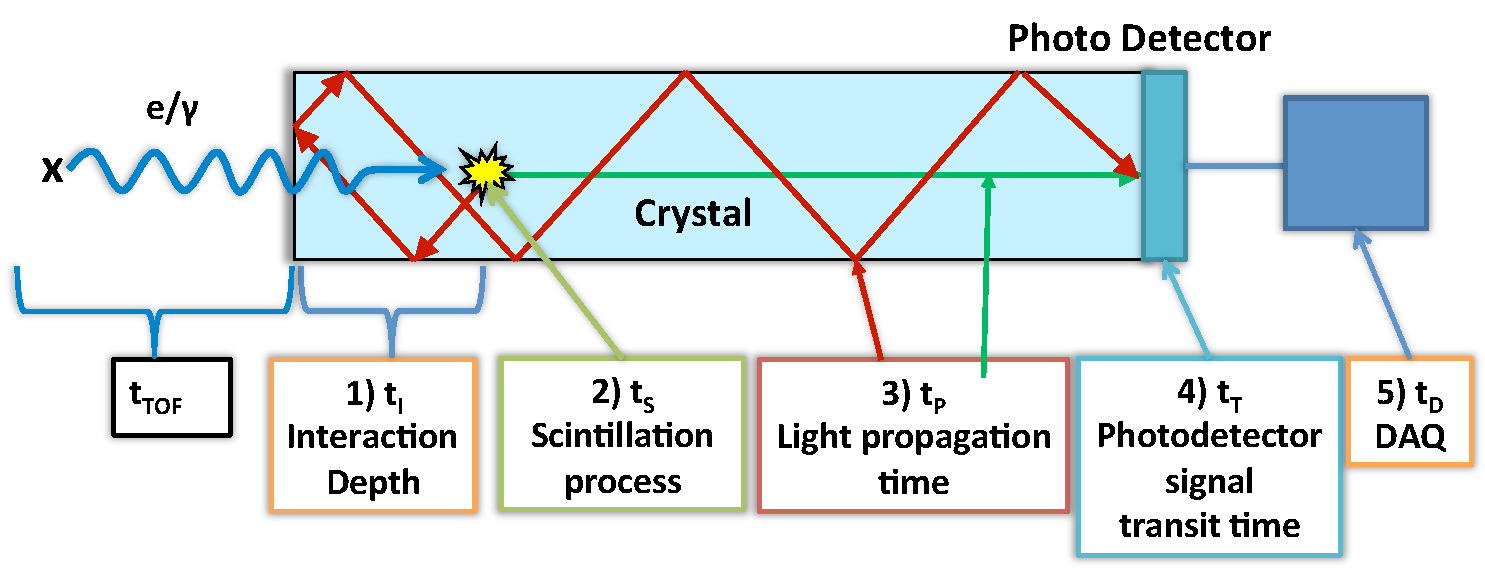
\includegraphics[width=0.85\textwidth]{figs/ScintillatorTiming_v2}
\caption{Factors influencing the precision of the timing measurement with a
monolithic, large scintillating crystal. The incident particle impinges on the
crystal face from the left. Characteristic times of various factors are defined
in the colored boxes and in the text.}
\label{fig:ScintillatorTiming}
\end{figure}


Past studies~\cite{MCPFastCaloNIMA}, measured the time resolution at different
absorber thicknesses for electron beams with energies varying from $12$ to
$32$~GeV, and showed that the time of arrival of the front of an electromagnetic
shower can be determined with a precision better than $20$~ps. The electronic
time resolution of the DAQ system was also measured to be about $6$~ps. Using
the same techniques that were used in those studies, we measured the time
resolution of the MCP-PMT photodetectors used in this paper to be between
$11$~ps and $14$~ps, depending on the exact device.

To further characterize the time resolution of a crystal-based calorimeter, we
study the contributions due to fluctuations in the scintillation process, and in
the optical transit to the photodetector. The signal extracted from the
photodetector is typically the superposition of the signal generated by many
scintillation photons arriving together. As a result, the effect of the
fluctuations associated with the creation and transit of each particular
scintillation photon will be reduced for a LYSO-based detector whose signal is
the average of a large number of scintillation photons. Thus, of particular
interest is the dependence of the time resolution due to fluctuations in the
optical transit on the amount of scintillation light produced.


\section{Experimental Equipment}

A schematic diagram of a typical time of flight measurement
is shown in Figure~\ref{fig:TypicalSchematicDiagram}. All
measurements involve a fast photodetector which serves to
measure the reference ($t_{0}$) timestamp, typically 
an MCP-PMT, and a photodetector further downstream
that detects the signal associated with the
electromagnetic shower from which a simultaneous energy 
and time ($t_{1}$) measurement is made. 

\begin{figure}[H] \centering
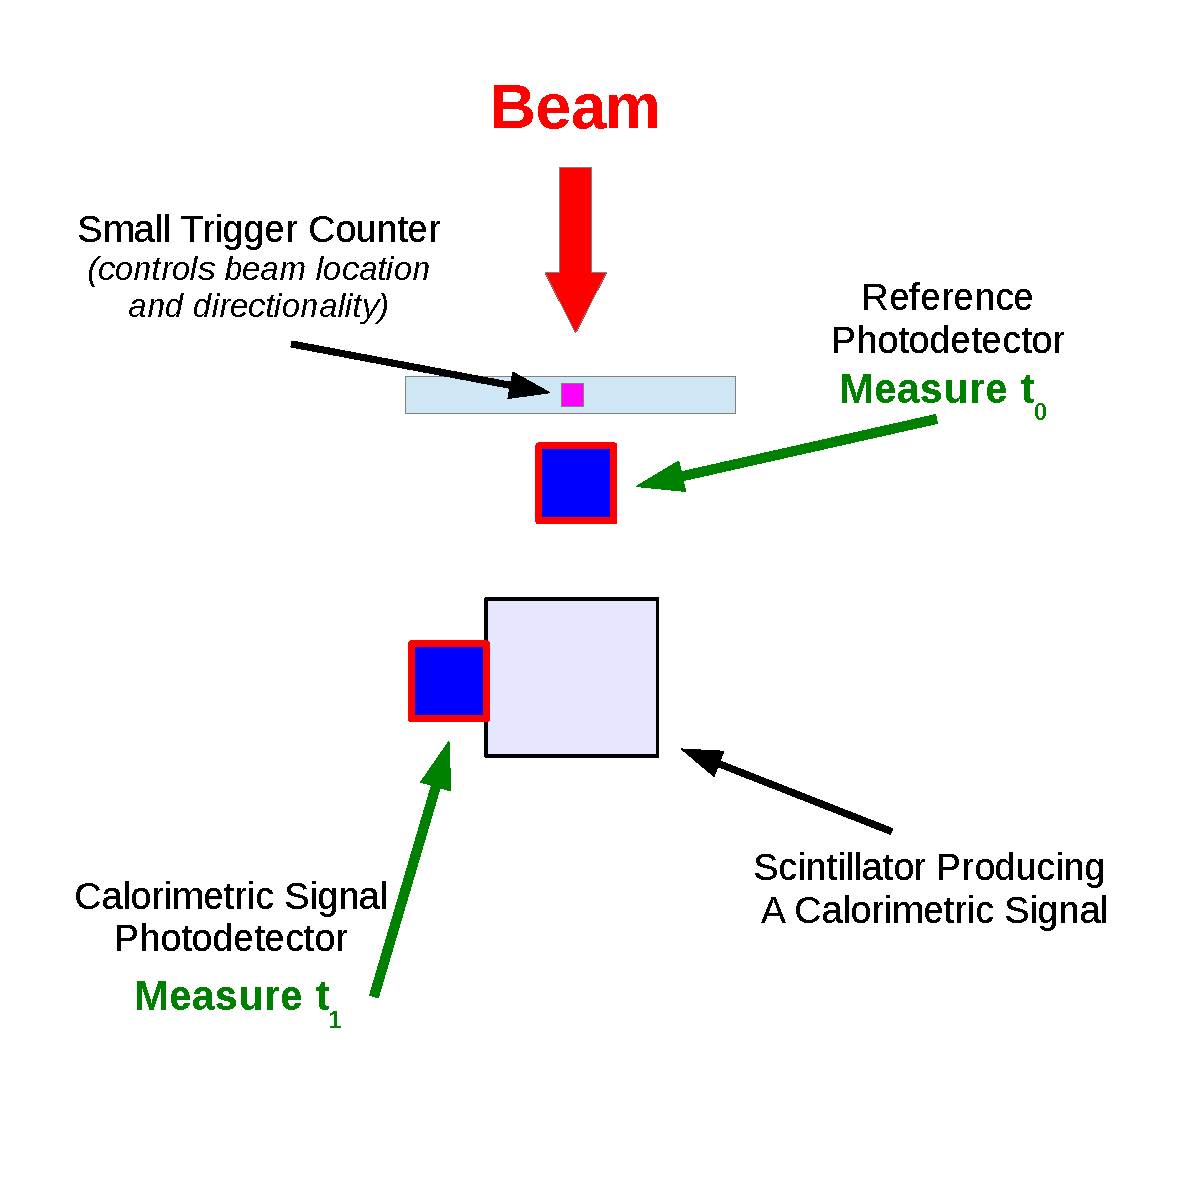
\includegraphics[width=0.45\textwidth]{figs/TypicalSchematicDiagram} 
\caption{A schematic diagram of the experimental setup for
a typical time of flight measurement is shown to illustrate the
basic detector elements.} 
\label{fig:TypicalSchematicDiagram}
\end{figure}

Two types of MCP-PMT photodetectors are used, one produced by Hamamatsu (model
R3809-52)~\cite{HamamatsuMCP3809}, and one produced by Photek (model
PMT240)~\cite{Photek240}. A version 4 DRS4 waveform digitizer evaluation
board~\cite{DRS4} was used as the primary DAQ system, connected to a laptop via
USB interface. All experimental beam studies were performed at the Fermilab Test
Beam Facility (FTBF), which provided proton beams from the Fermilab Main
Injector accelerator at $120$ GeV, and secondary electron beams of energies
ranging from $4$ to $32$~GeV. Detector elements were placed inside of a dark box
lined with copper foil, providing RF shielding. A $2$x$2$~$\mathrm{mm}^{2}$
scintillator is placed inside the box at the upstream extremity and used to
trigger the DAQ readout, providing a relatively strict constraint on the
location and directionality of the beam particles used in the time of flight
studies. Finally, the differential Cherenkov counter provided by the FTBF
facility and located upstream of our experimental hall, is used for electron
identification. 

\section{Event Selection and Analysis}

The analyses performed in these studies primarily involve reconstructing the
time of flight of beam particles between different detector elements. Slightly
different algorithms are used for different detector elements, but all involve
the assignment of a timestamp using specific features of each corresponding
signal pulse. The signal pulse for the reference time detector is typically very
sharp and relatively symmetric around its maximum amplitude, as shown in
Figure~\ref{fig:PulseShapes}. Therefore, for the reference detector we determine
the time position of the pulse peak and fit a Gaussian function to the peak of
the pulse, using three sampling points before the pulse maximum and four
sampling points after. The best fit mean parameter of the Gaussian function is
assigned as the timestamp $t_{0}$. The signal pulse for the downstream time
measurement is typically the result of scintillation light, and exhibits a
relatively fast rising edge and a significantly slower decay. Therefore, we
assign the timestamp $t_{1}$ using a constant fraction of the rising edge. A
linear function is fit to the sampling points between $10\%$ and $60\%$ of the
pulse maximum and the timestamp is assigned as the time at which the best-fit
linear function rises to $20\%$ of the pulse maximum. Examples of fits performed
to assign a time stamp from each pulse are shown in Figure~\ref{fig:PulseFits}.
In both cases, some optimization was performed to arrive at the exact algorithm
parameters used.

\begin{figure}[h] \centering
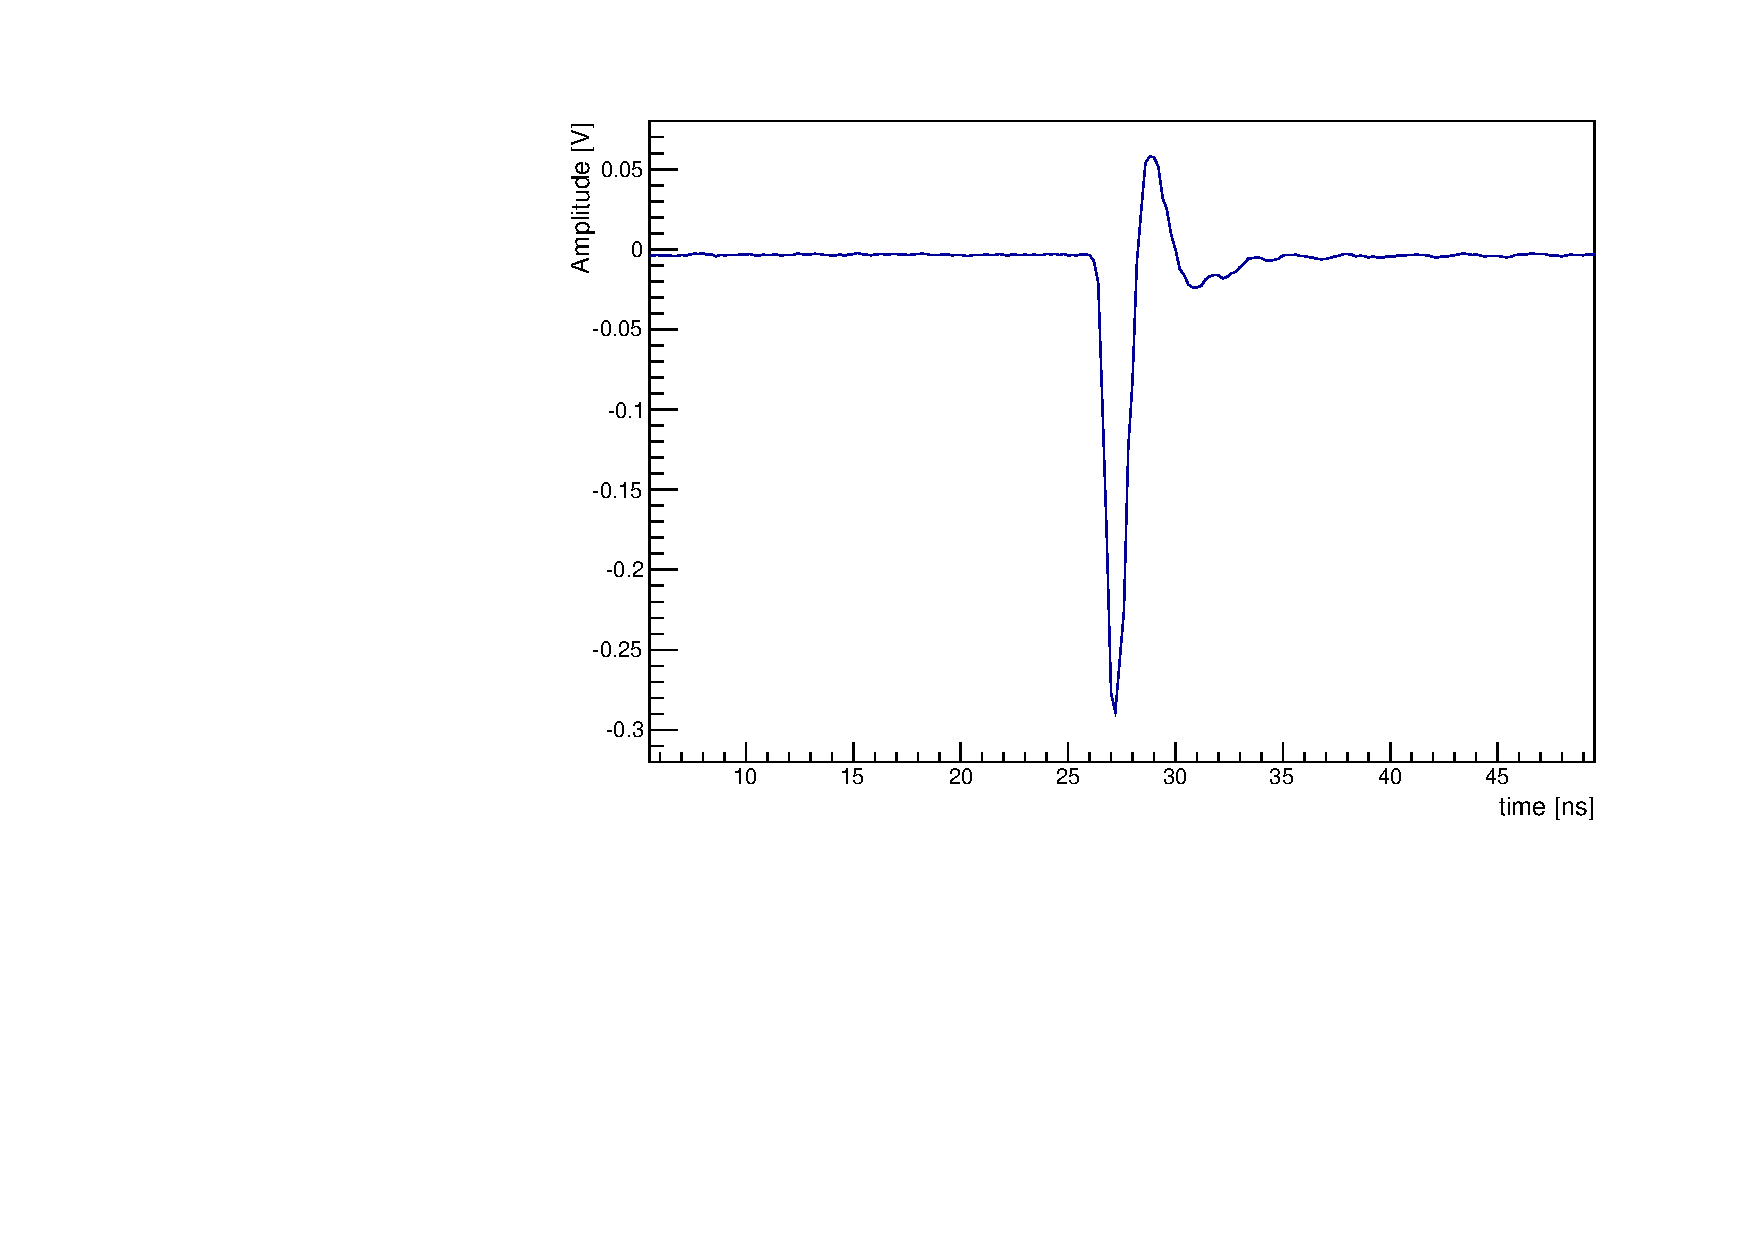
\includegraphics[width=0.45\textwidth]{figs/RefPulse} 
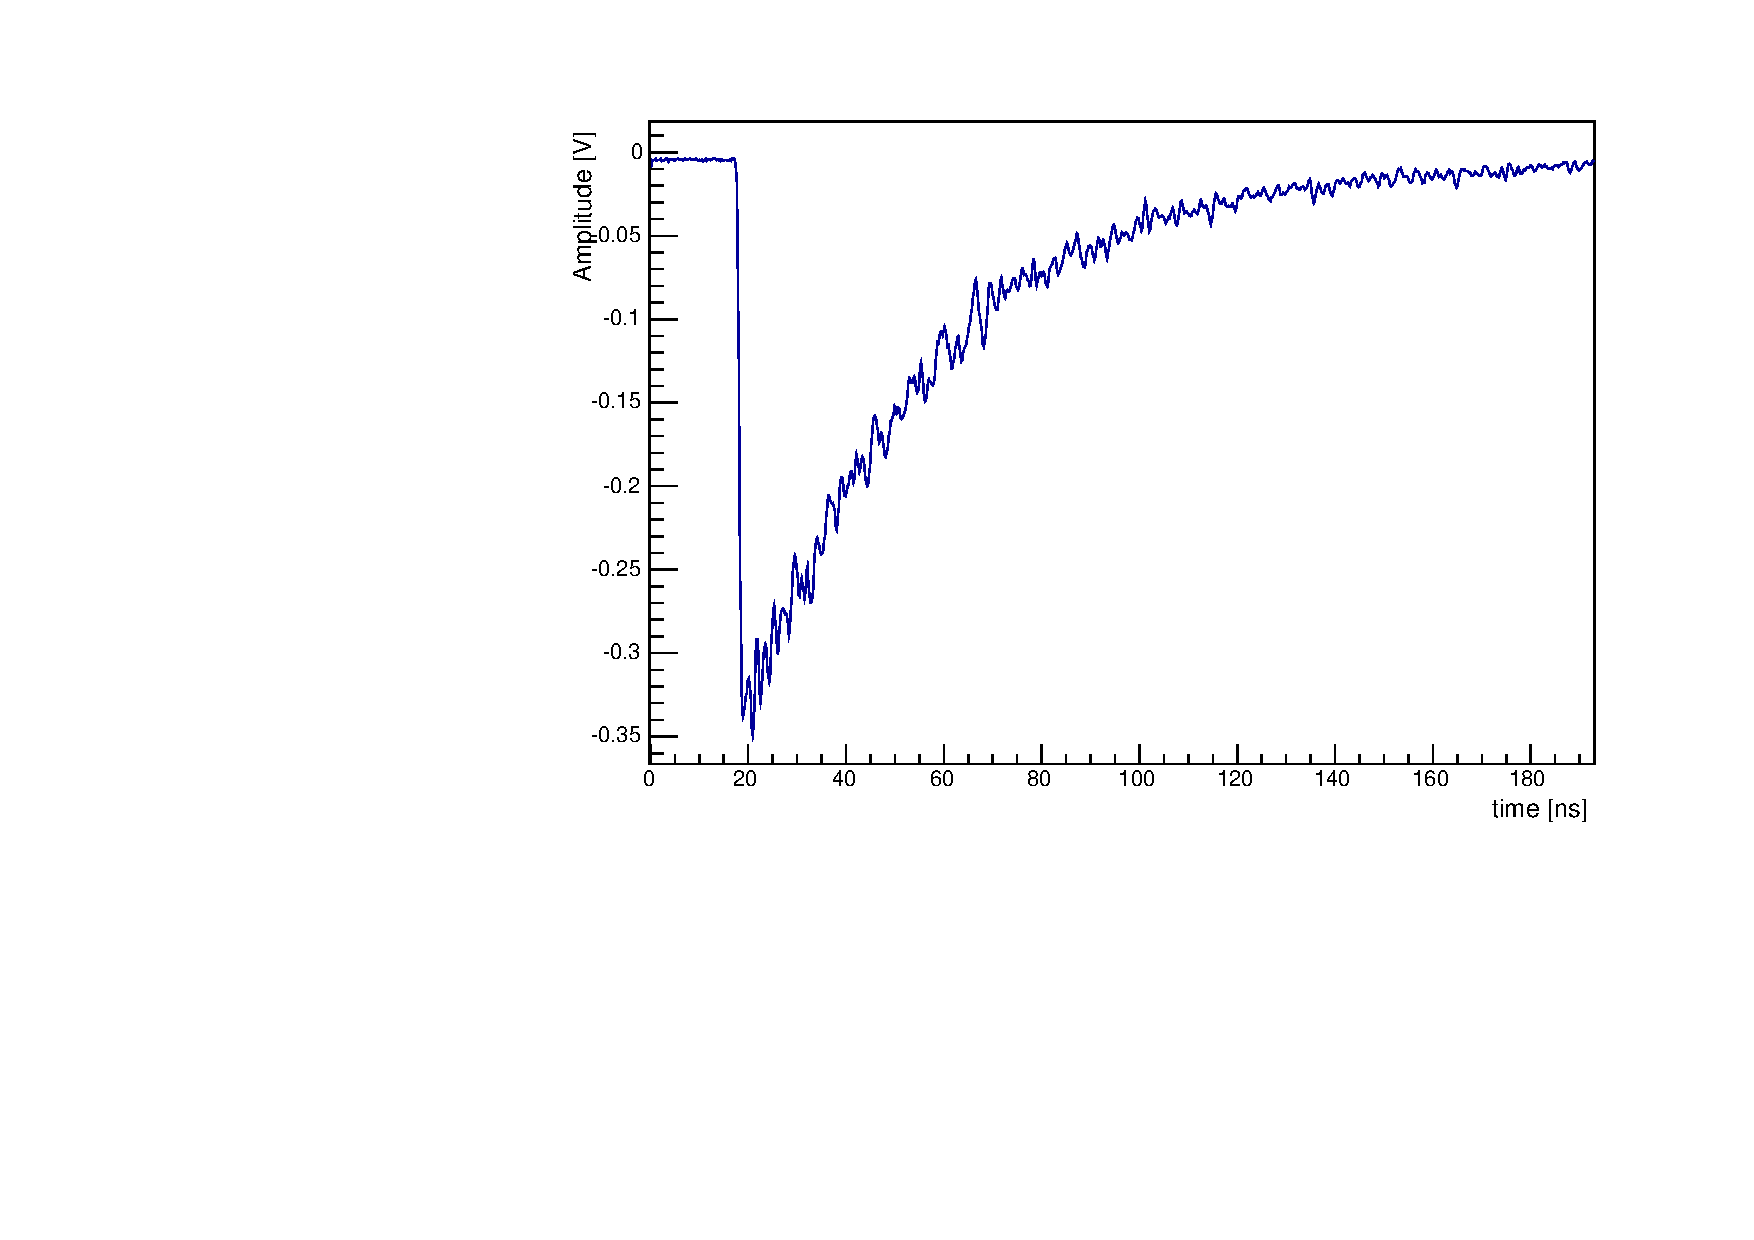
\includegraphics[width=0.45\textwidth]{figs/run064_event506} 
\caption{Sample pulses as digitized by the DRS4 board. 
On the left is a  pulse from the reference Photek 240 MCP-PMT, 
and on the right is a pulse from the Hamamatsu R3809 MCP-PMT
optically coupled to a (1.7~cm)$^{3}$ LYSO crystal 
recorded during an 8 GeV electron run.} 
\label{fig:PulseShapes}
\end{figure}

Event selection and pulse cleaning procedures are used to eliminate abnormal
pulses in the readout. Large signals above 500 mV are also rejected because they
saturate the DRS4 inputs. Only pulses with amplitude larger than 20 mV are used
for time of flight measurements, in order to reduce the impact of noise from the
DRS waveform digitizer DAQ system. Events containing more than one pulse within
the $200$~ns readout window are not used. 

\begin{figure}[h] \centering
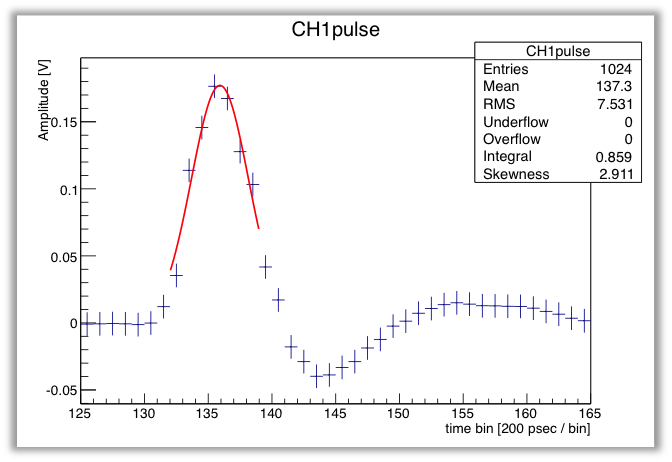
\includegraphics[width=0.45\textwidth]{figs/RefPulseFit} 
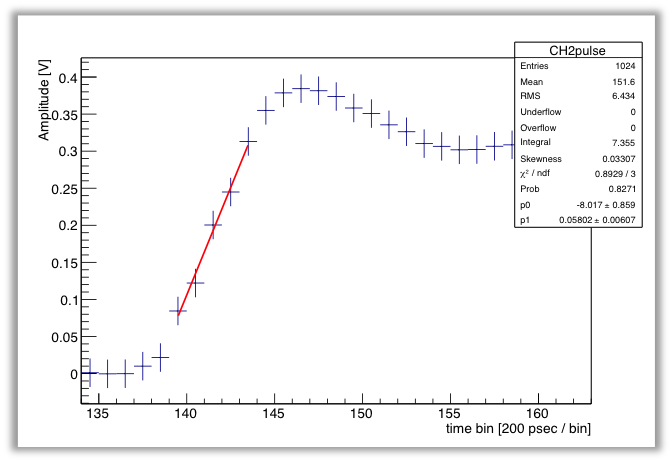
\includegraphics[width=0.45\textwidth]{figs/ScintPulseFit} 
\caption{Sample fits used to assign timestamps to digitized MCP-PMT pulses. 
On the left is a pulse from the reference Photek 240 MCP-PMT, and
on the right is a pulse from the Hamamatsu R3809 MCP-PMT
optically coupled to a (1.7~cm)$^{3}$  LYSO crystal
recorded during an 8 GeV electron run.}
\label{fig:PulseFits}
\end{figure}


\section{Timing in LYSO Crystal-based Calorimeters}

Besides the effects of the photodetector and DAQ electronics, timing in
LYSO-based calorimeters is driven by three factors: shower profile fluctuations,
scintillation, and optical transport. Stochastic processes during the
development of an electromagnetic shower affect the time of observed signals, as
both the transverse size and the depth of the shower can fluctuate event by
event. Random processes in the scintillation mechanism and the randomization of
the optical paths for the scintillation light affect both the speed of the
signal formation and the time jitter. We study these effects using two
independent experimental setups. 

For a traditional homogeneous crystal calorimeter, optical transit effects are
significant because scintillation light must travel a long distance down the
length of the crystal to reach the photodetector. We start with a setup which
uses an LYSO cube with linear dimensions of $1.7\mathrm{cm}$ as the active
scintillation element. The small size of this element reduces the effect of
optical transit jitter. The LYSO cube is placed behind about $4.5$ radiation
lengths of lead. Using this LYSO-based sampling calorimeter, we measure the time
resolution of electrons.

Second, we study a shashlik calorimeter composed of alternating layers of
tungsten and LYSO, in which scintillation light is extracted through wavelength
shifting (WLS) fibers. In this setup, optical transit through the fiber is the
dominant factor for timing. Additionally, we study an alternate version of this
calorimeter in which light is extracted through direct optical coupling of
photodetectors to the edges of a few LYSO layers. In this setup, optical transit
effects are less dominant.



\subsection{Timing Studies of the LYSO-based Sampling Calorimeter}

We study the combined impact of the shower profile fluctuations, the
scintillation mechanism in LYSO, and the optical transit on the time resolution
using a sampling calorimeter with a (1.7~cm)$^{3}$ LYSO cube as active
element. The LYSO crystal is wrapped in Tyvek and attached to the Hamamatsu
R3809 MCP-PMT with optical coupler~\cite{grease}, which is used as a time reference. A Photek 240
MCP-PMT is placed upstream of the calorimeter and is used to measure the
reference time. A schematic diagram and a photograph of the experimental setup
are shown in Figure~\ref{fig:LYSOSamplingCaloSetup}. 

\begin{figure}[h] \centering
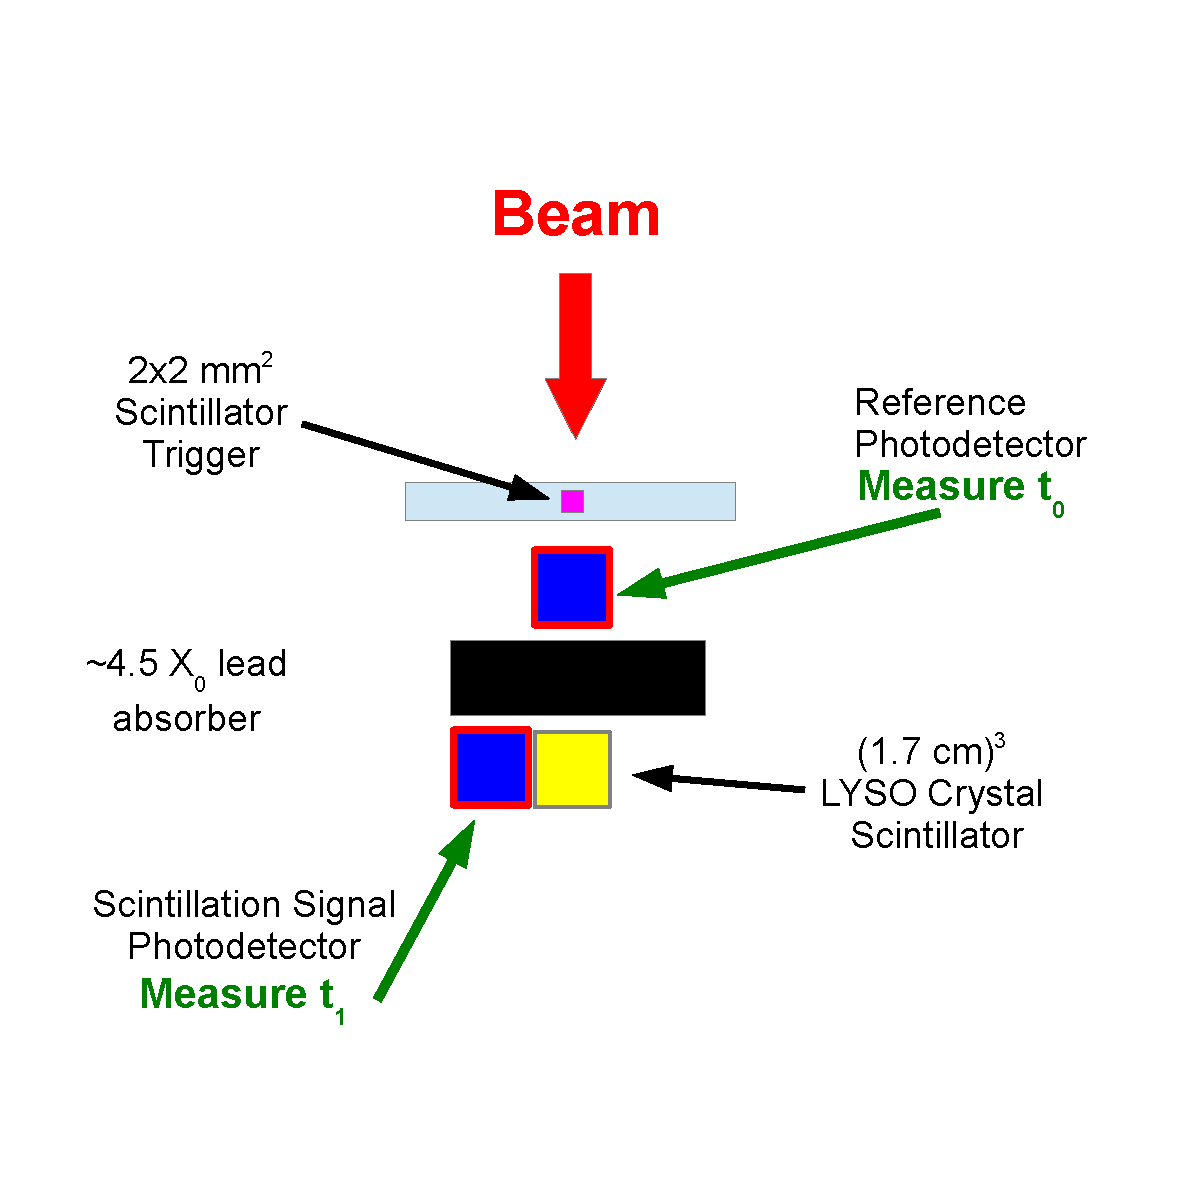
\includegraphics[width=0.45\textwidth]{figs/LYSOSamplingCaloSetupSchematic} 
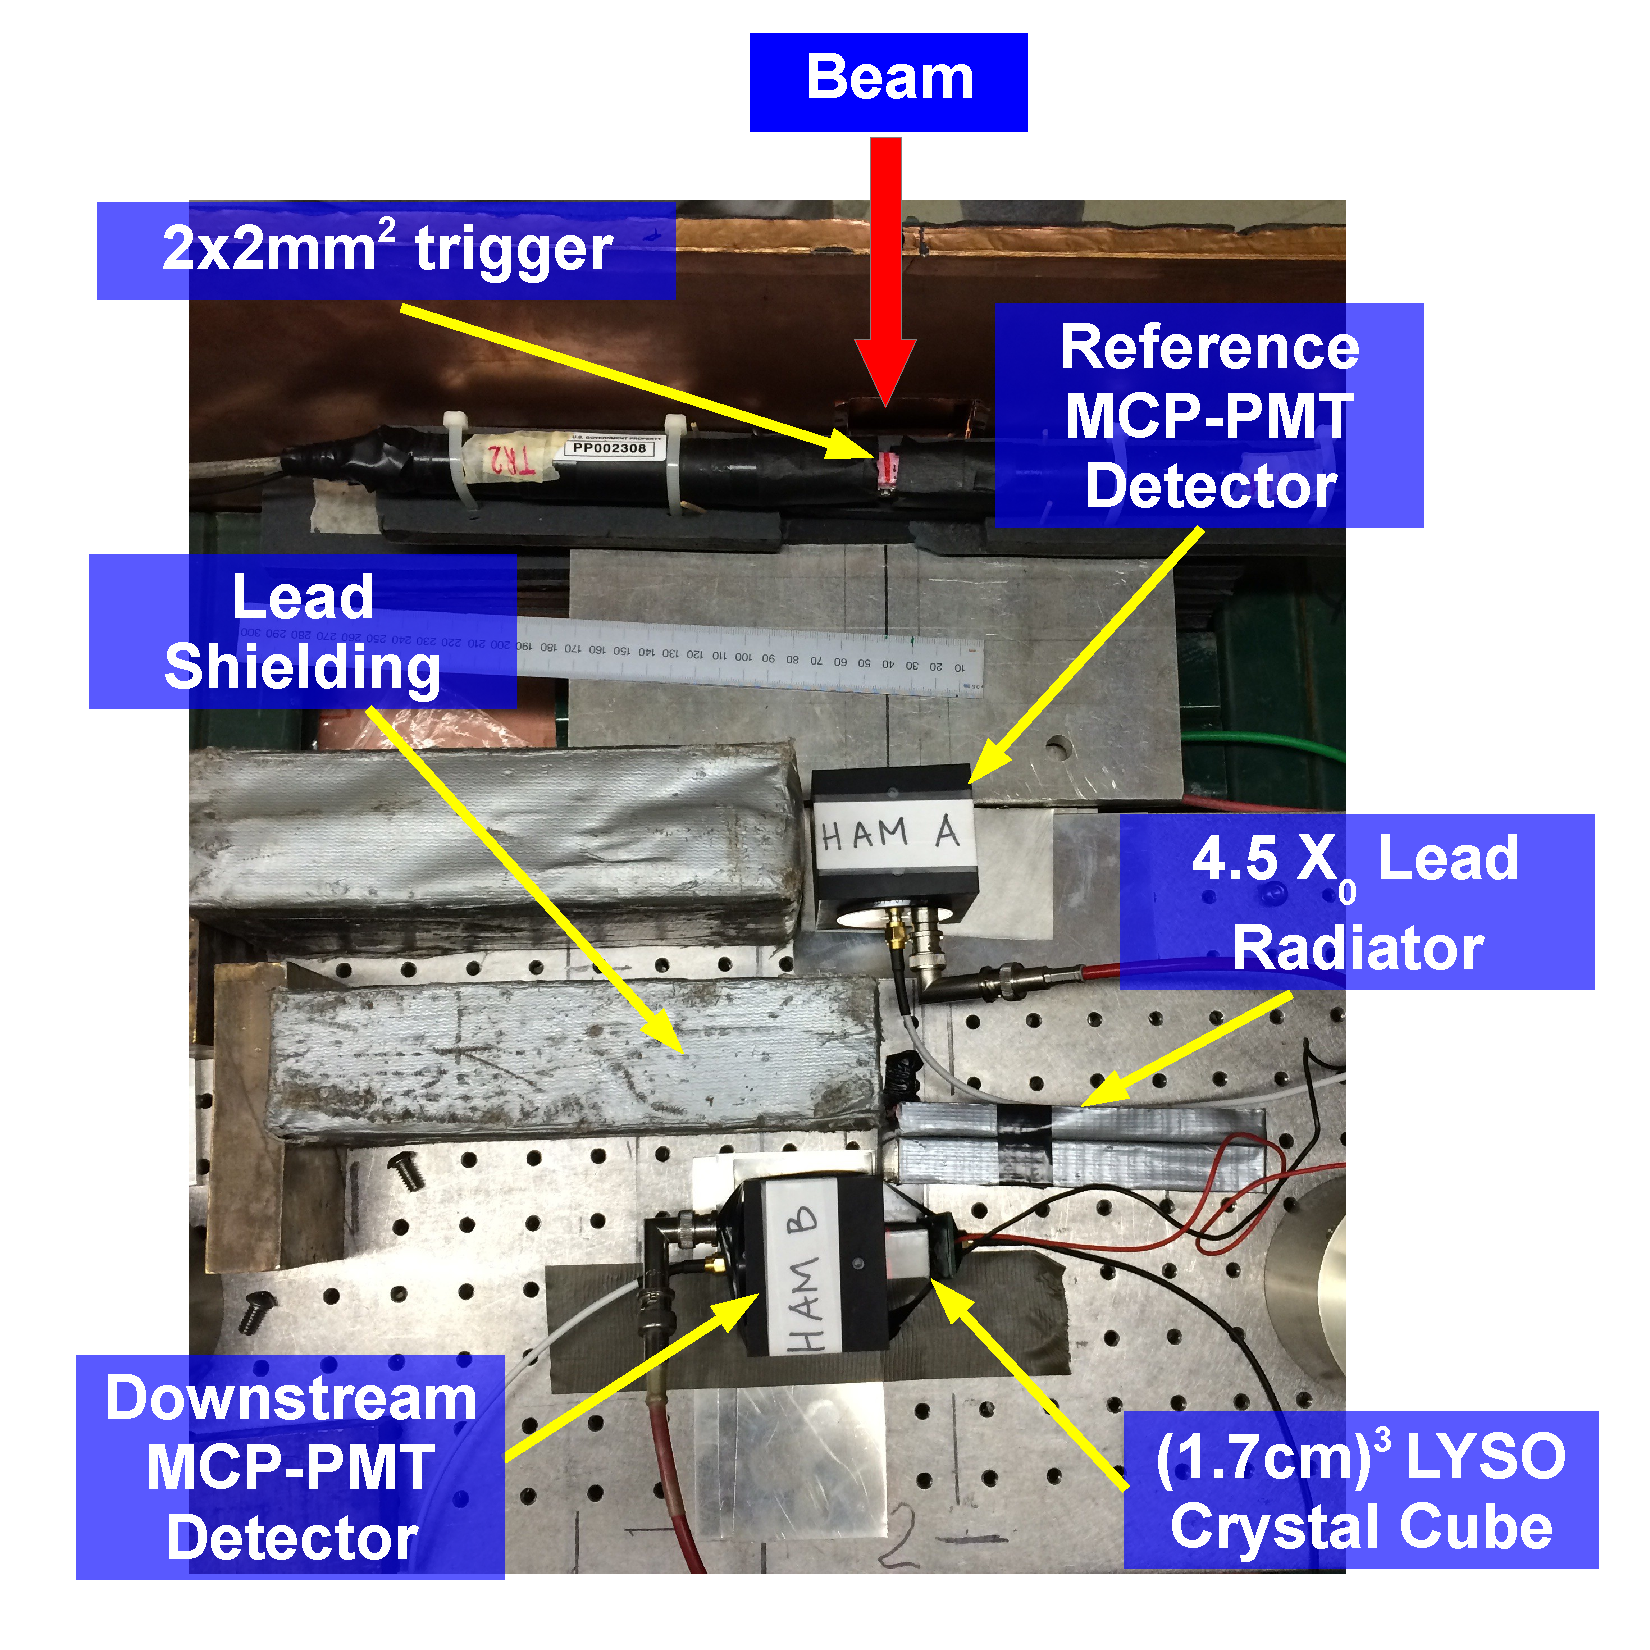
\includegraphics[width=0.45\textwidth]{figs/LYSOSamplingCaloSetupPhoto} 
\caption{ A schematic diagram of the experimental setup for the
time of flight measurement using the LYSO sampling calorimeter is shown
on the left, along with a photograph of the experimental setup shown on the right. } 
\label{fig:LYSOSamplingCaloSetup}
\end{figure}

A plastic scintillator, approximately $2$~mm by $2$~mm in cross sectional area
and placed upstream of the reference time detector, is used to trigger the DAQ
readout on the DRS waveform digitizer and ensures that the electron beam is
constrained to within a $2\times 2$~mm$^2$ region. Electron events are identified by
requiring a signal with amplitude larger than $10$~mV in the Cherenkov counter.
Finally, large lead bricks are placed upstream of the Hamamatsu R3809 MCP-PMT,
out of the path of the beam. These shield the photodetector from stray particles
produced in events where an electromagnetic shower occurs upstream of the lead
radiator. Such stray shower particles yield very fast signals which can
significantly contaminate the scintillation signal. Using the same experimental
setup without the LYSO active element in place, we find that stray shower type
events yield less than $10\%$ contamination and give a negligible effect on the
scintillation signal. The same calorimeter setup with the Photek 240 MCP-PMT in
place of the Hamamatsu R3809 MCP-PMT, which has an active area about $10$ times
larger, is found to yield more than $80\%$ contamination and thus does not allow
a proper measurement of the scintillation signal.

Although the thickness of the LYSO active element is relatively small and
captures only a fraction of the total energy of the electron, the location of
the active element is relatively close to the shower maximum for electromagnetic
showers, and yields a reasonable energy measurement. In
Figure~\ref{fig:LYSOCubeEnergy32GeV} we show the distribution of the MCP-PMT
pulse integral, a quantity proportional to the total collected charge, for
$32$~GeV electron beam events recorded by out setup. We find a resolution of
about $20\%$.


\begin{figure}[h] \centering
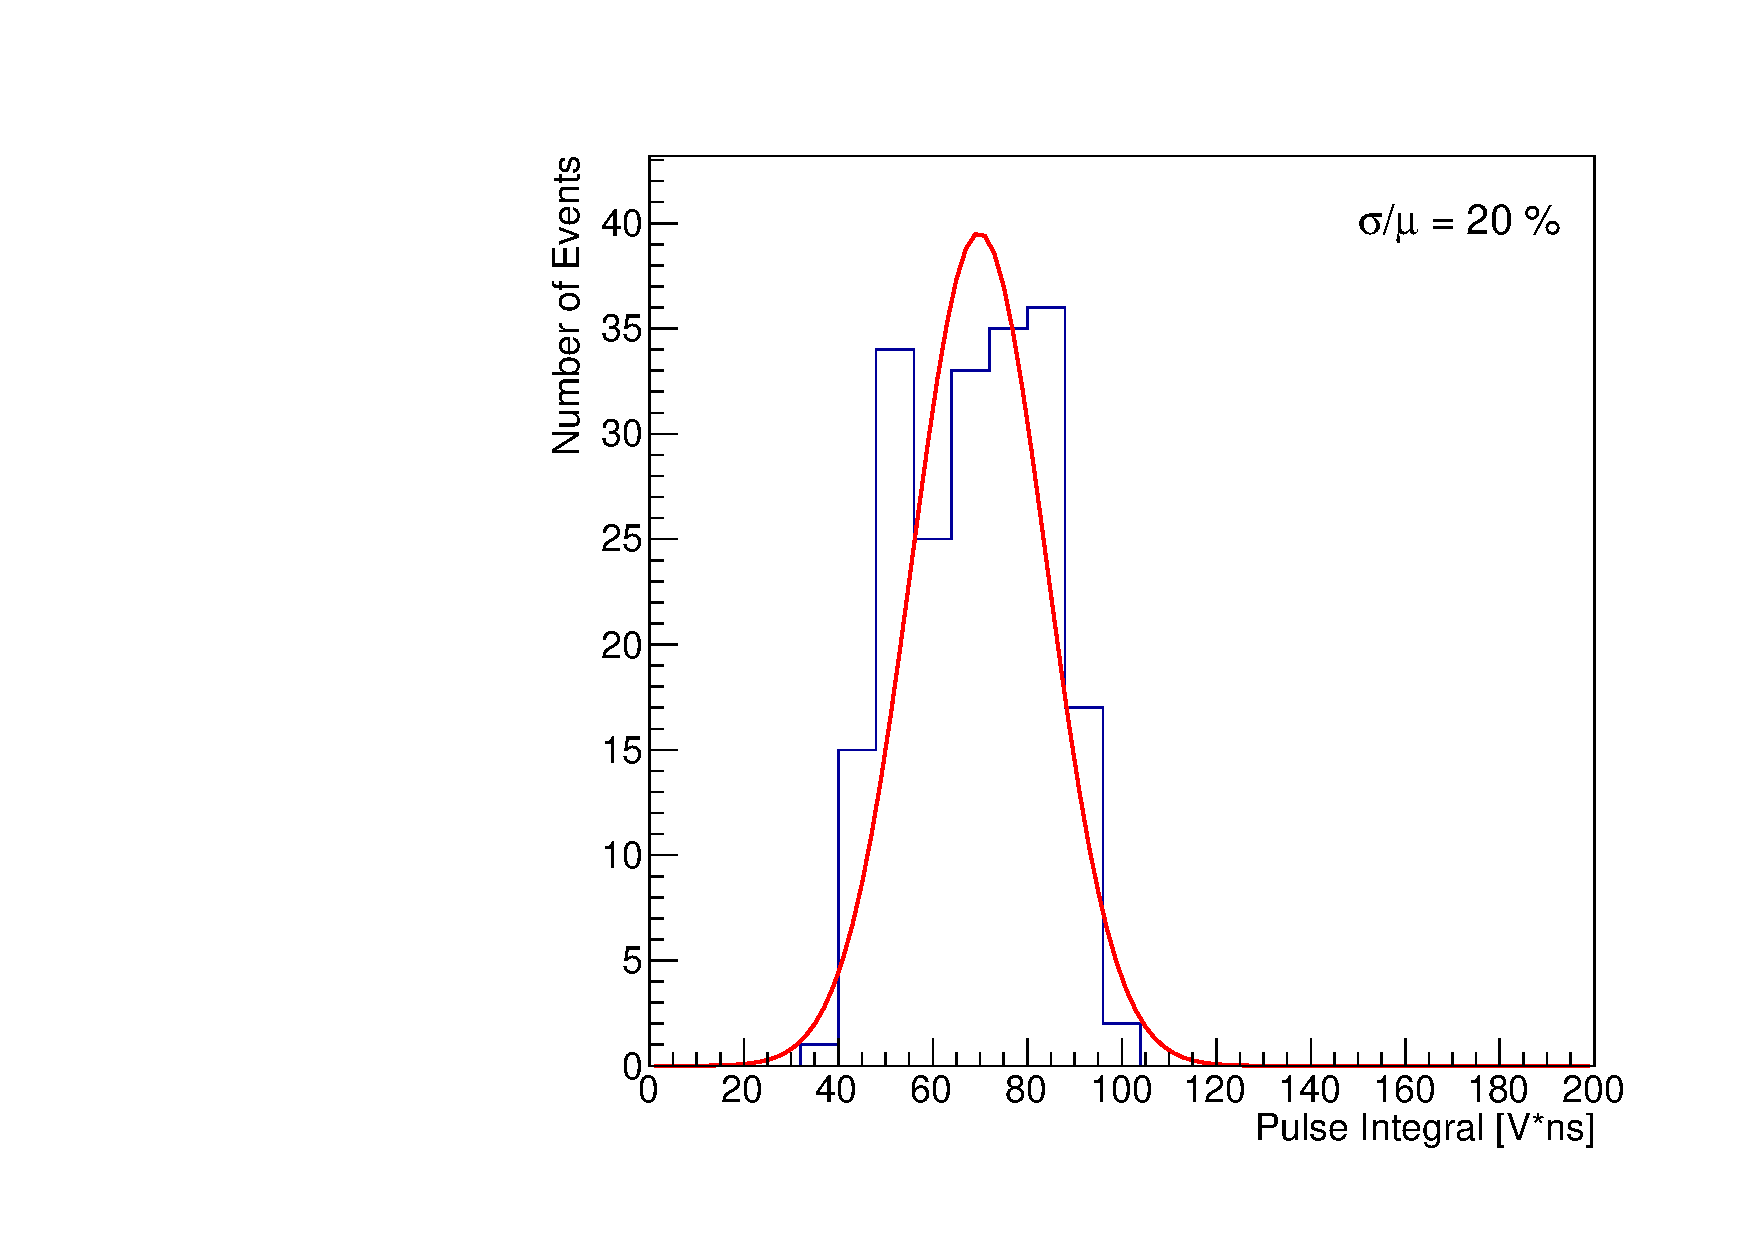
\includegraphics[width=0.45\textwidth]{figs/TOF_Electron_LYSOCube_32GeV_energy} 
\caption{ Histogram of the pulse integral for events recorded using
the LYSO cube sampling calorimeter for a $32$~GeV electron beam. A
$50$~$\Omega$ termination is used for signals outputted by the MCP-PMT
photodetectors. } 
\label{fig:LYSOCubeEnergy32GeV}
\end{figure}

The time of flight measurement is performed using the LYSO sampling calorimeter
for electron beams with energies varying from $4$~GeV to $32$~GeV. The 
measured time of flight distributions are shown in Figure~\ref{fig:LYSOCubeTOF}.
We achieve the best time resolution of $34$~ps for electrons
with beam energy of $32$~GeV.

\begin{figure}[H] \centering
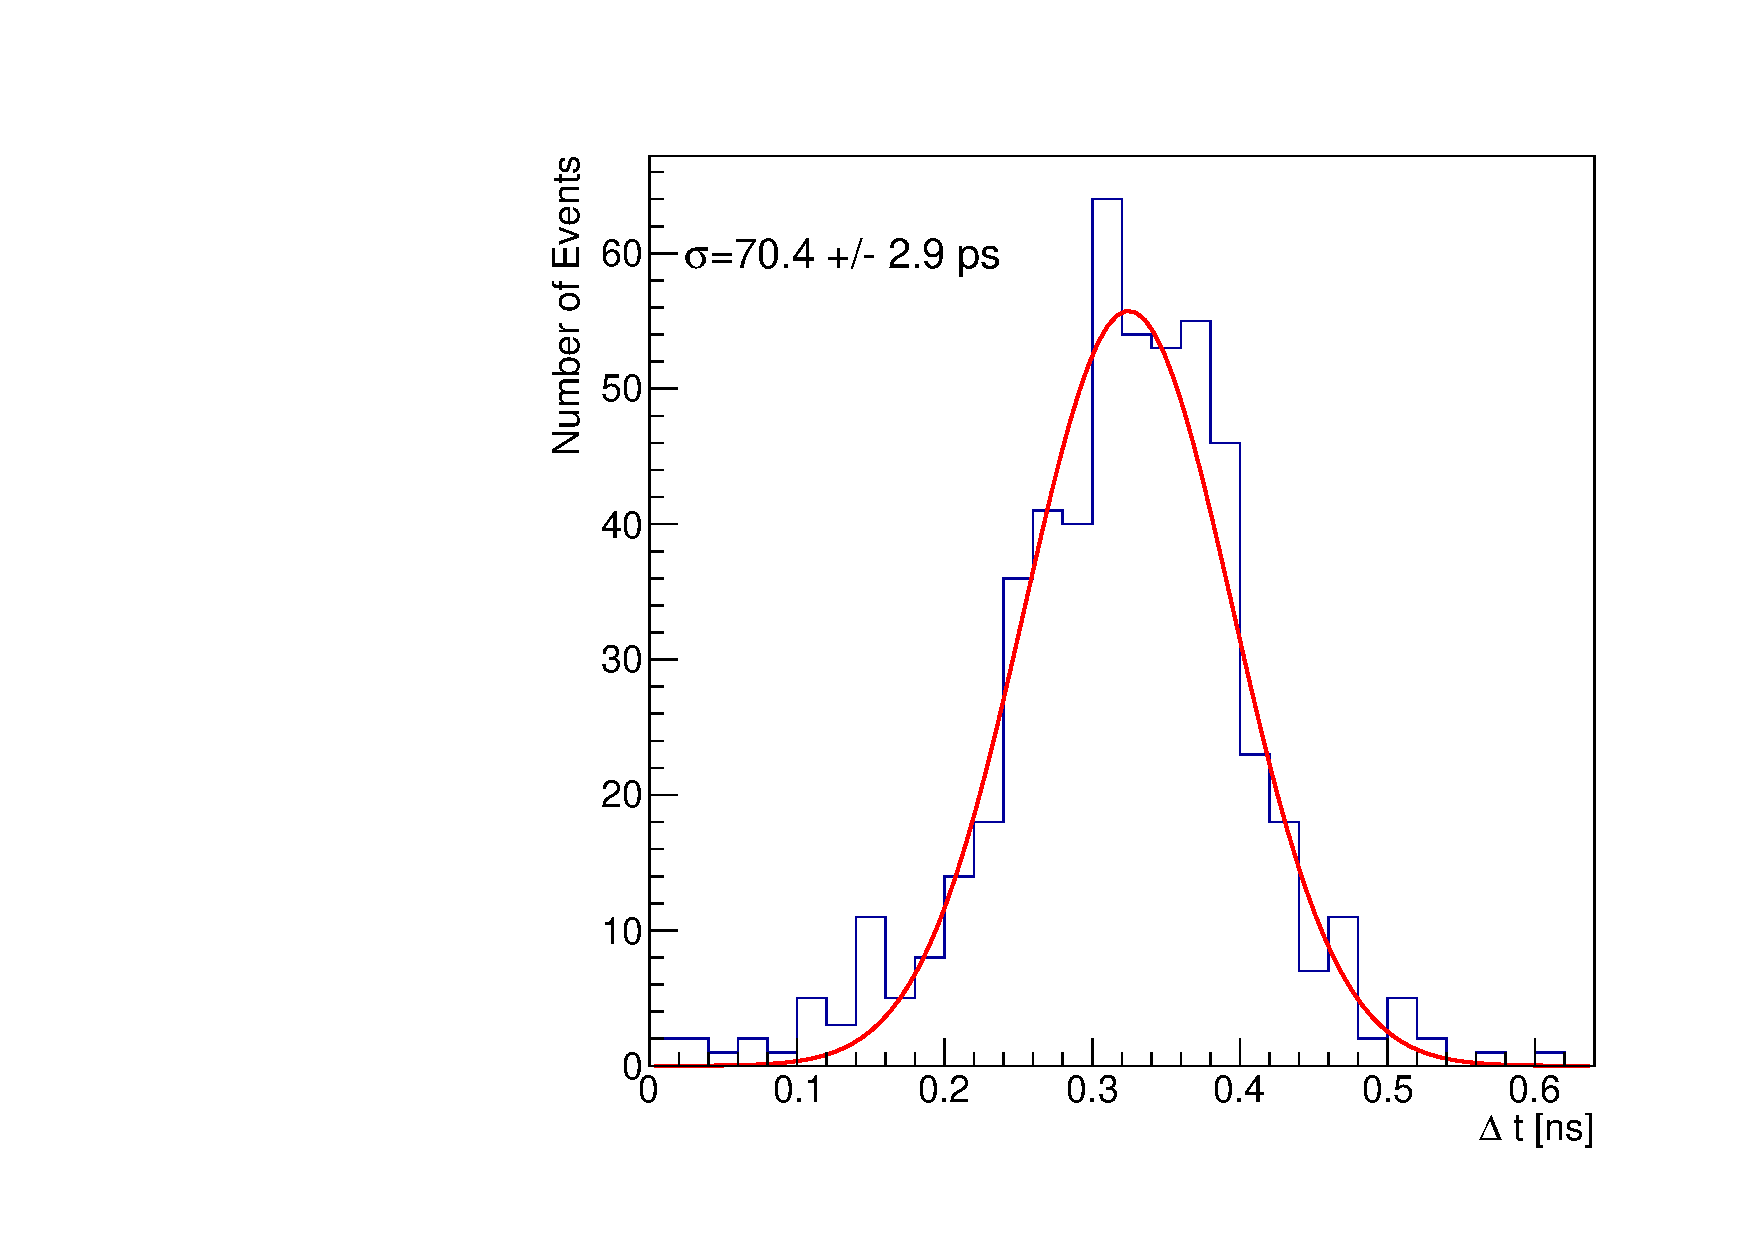
\includegraphics[width=0.45\textwidth]{figs/TOF_Electron_LYSOCube_4GeV} 
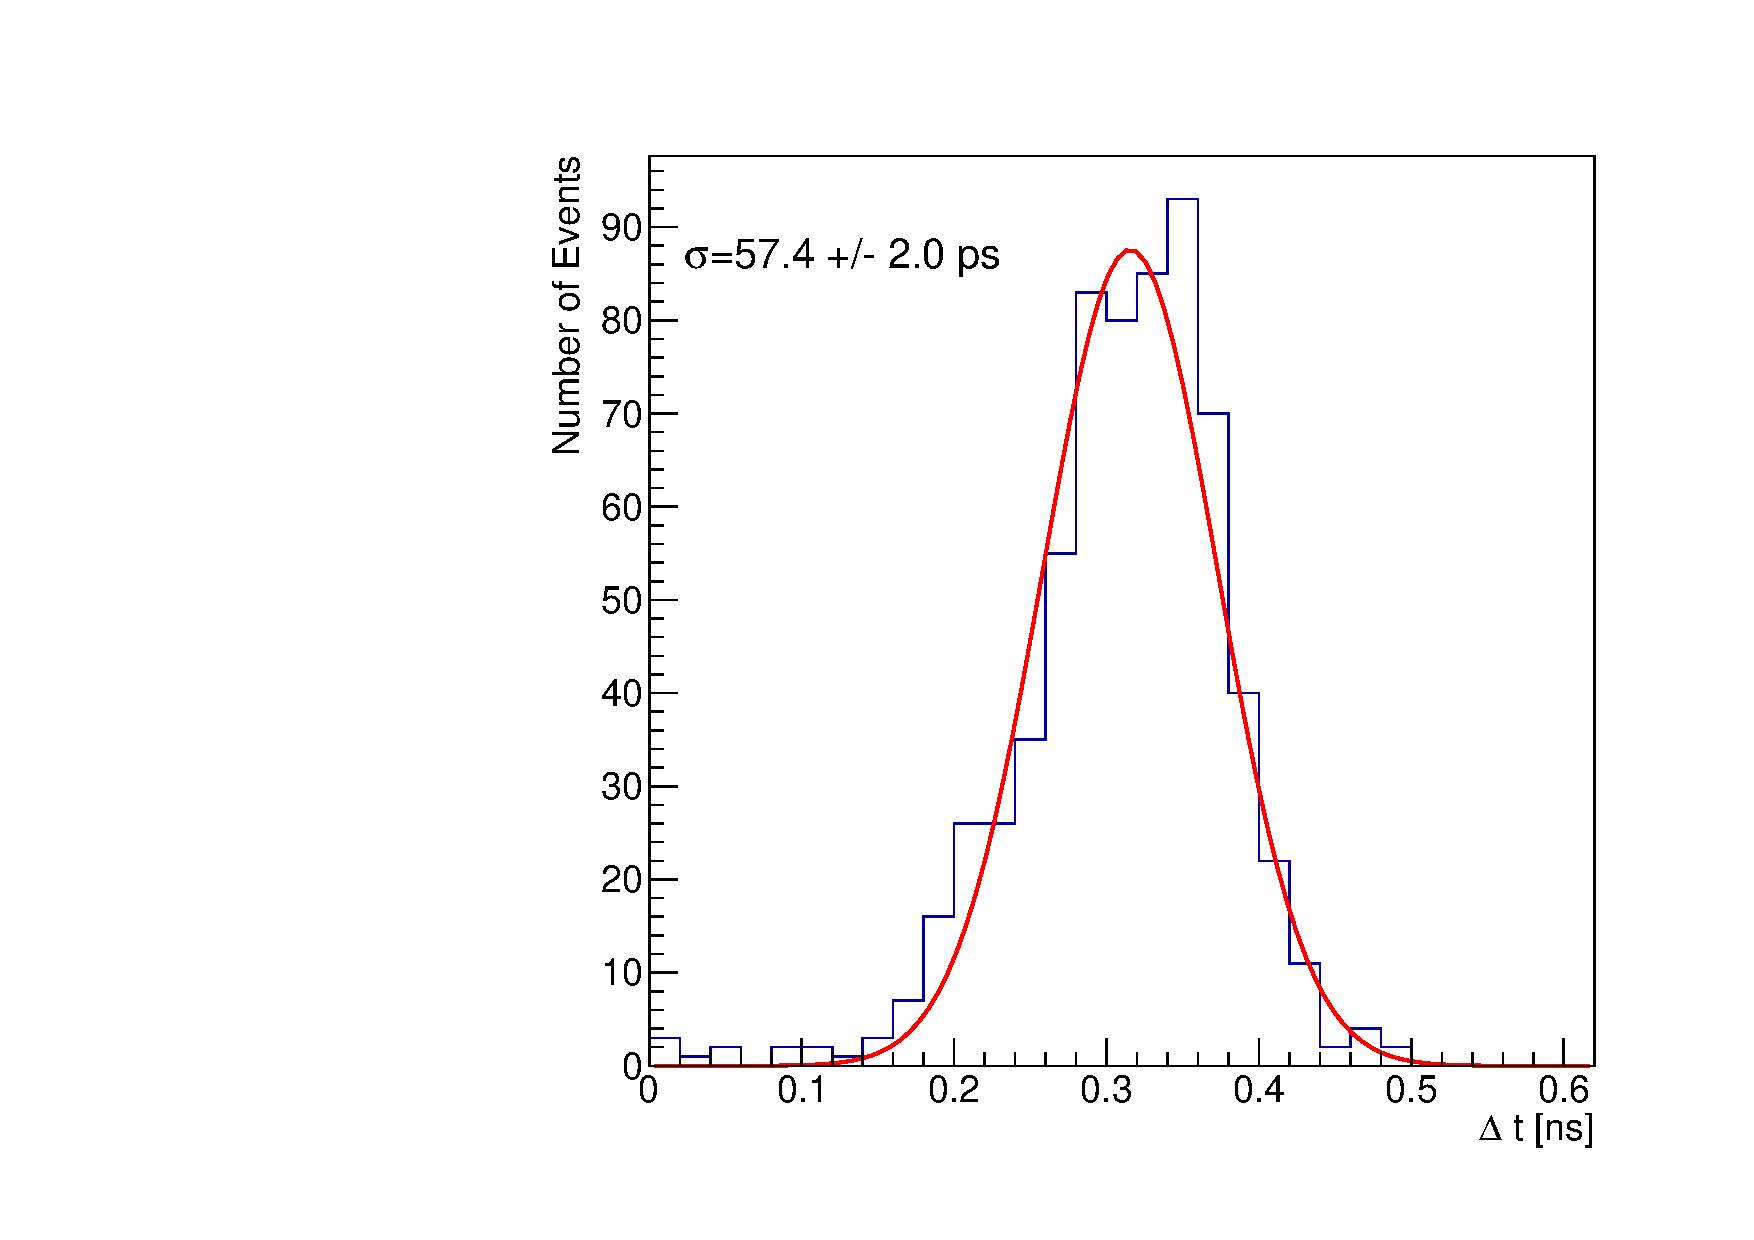
\includegraphics[width=0.45\textwidth]{figs/TOF_Electron_LYSOCube_8GeV} 
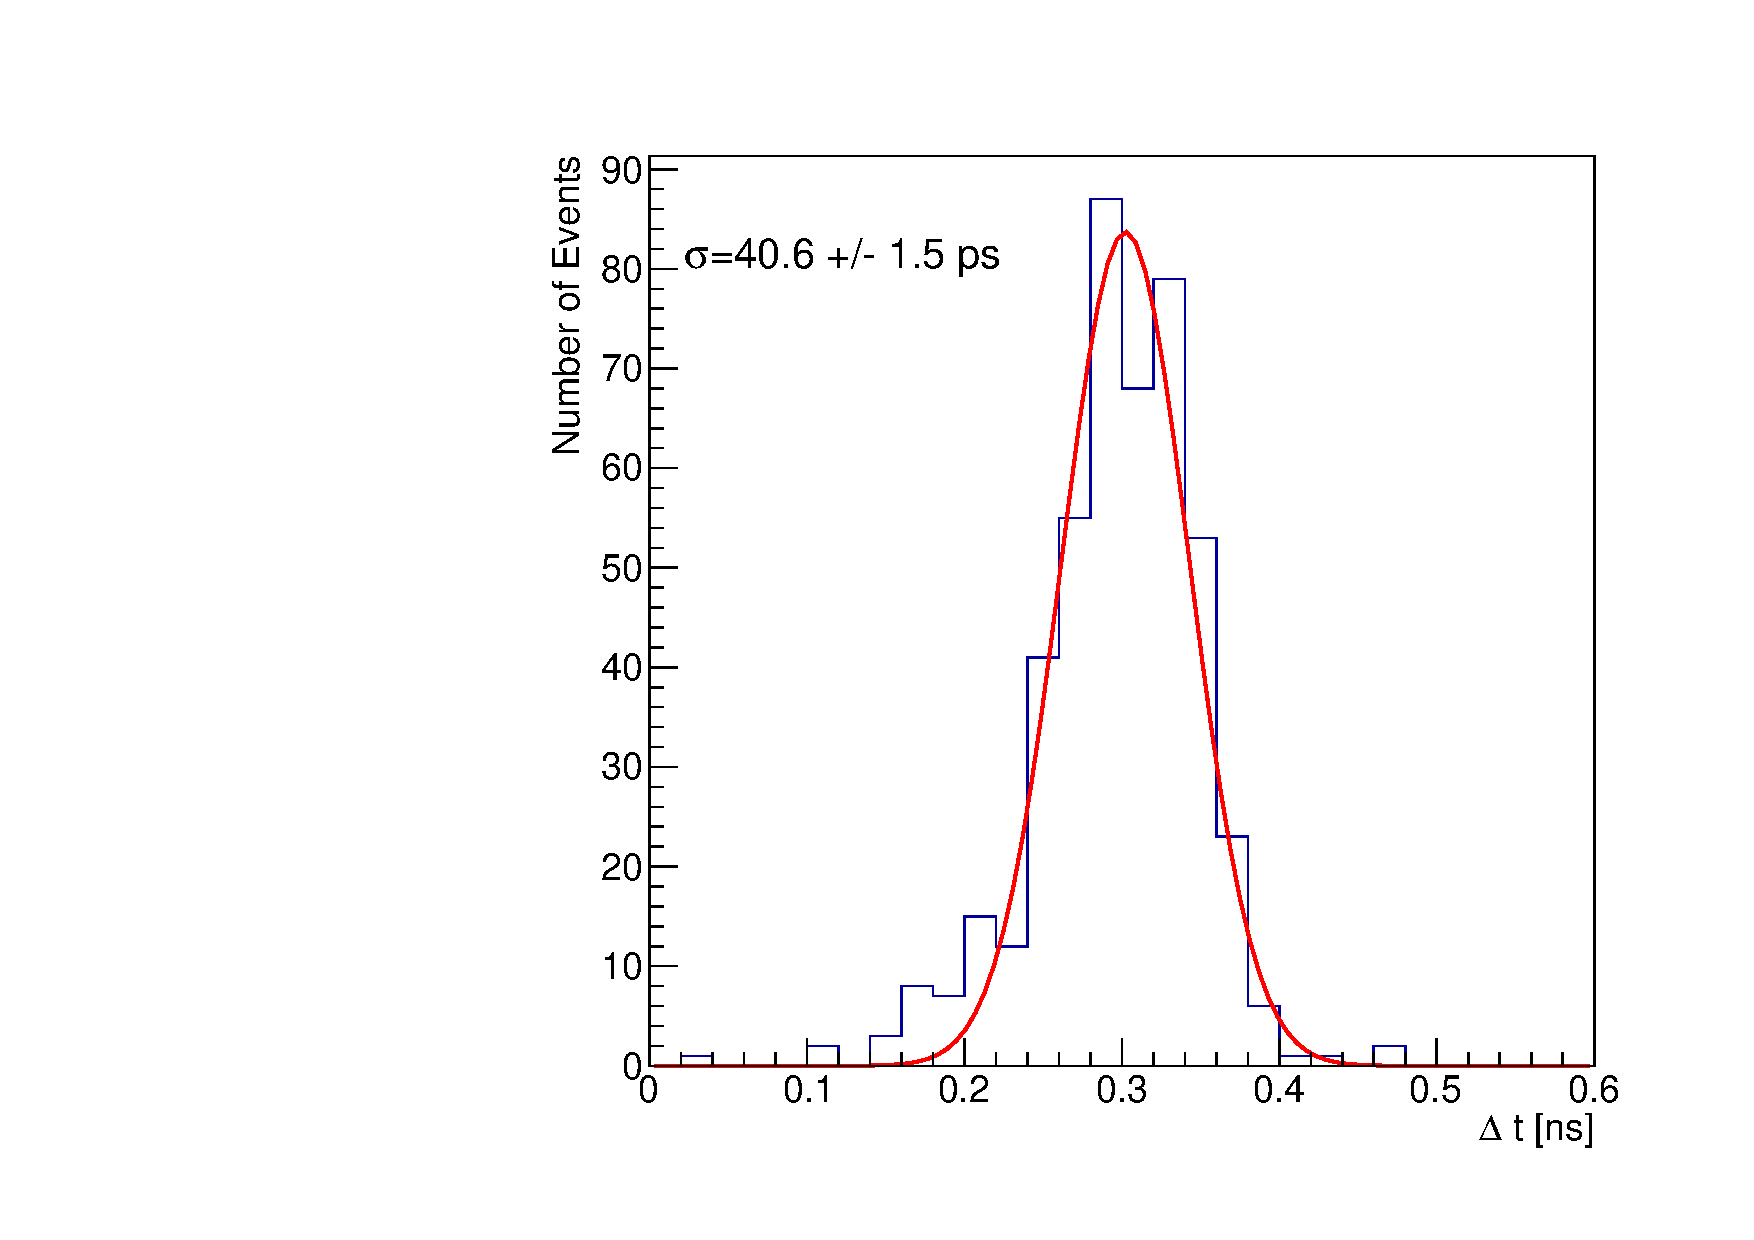
\includegraphics[width=0.45\textwidth]{figs/TOF_Electron_LYSOCube_16GeV} 
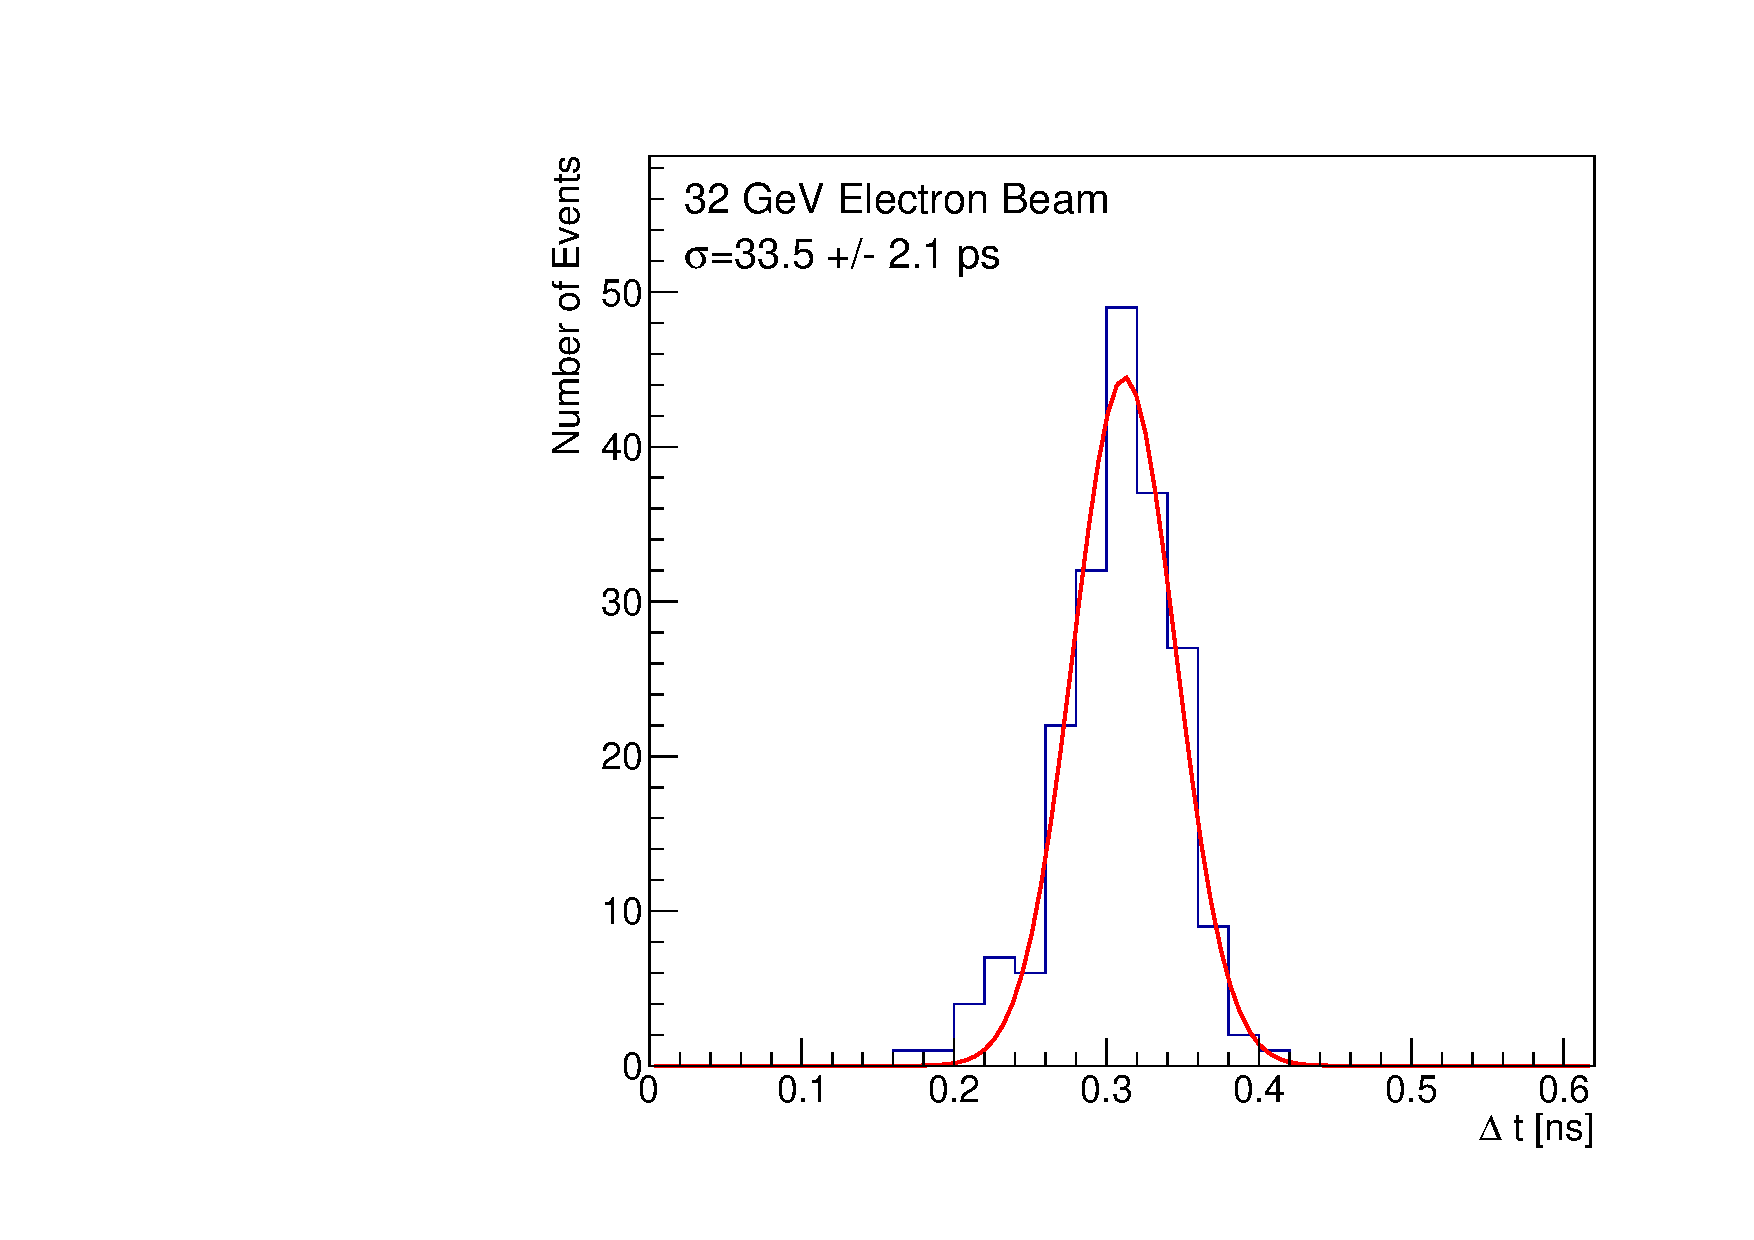
\includegraphics[width=0.45\textwidth]{figs/TOF_Electron_LYSOCube_32GeV} 
\caption{ Time of flight distributions for the LYSO cube sampling calorimeter
for electron beams with varying energies. } 
\label{fig:LYSOCubeTOF}
\end{figure}

The time resolution measurements are plotted as a function of the
beam energy in Figure~\ref{fig:LYSOCubeTOFResolutionVsEnergy}, and are observed
to follow a $1/\sqrt{E}$ dependence. We fit the result to the sum of a 
$1/\sqrt{E}$ term and a constant term, finding a constant term of
about $11$~ps with a statistical uncertainty of about $30\%$. 

\begin{figure}[h] \centering
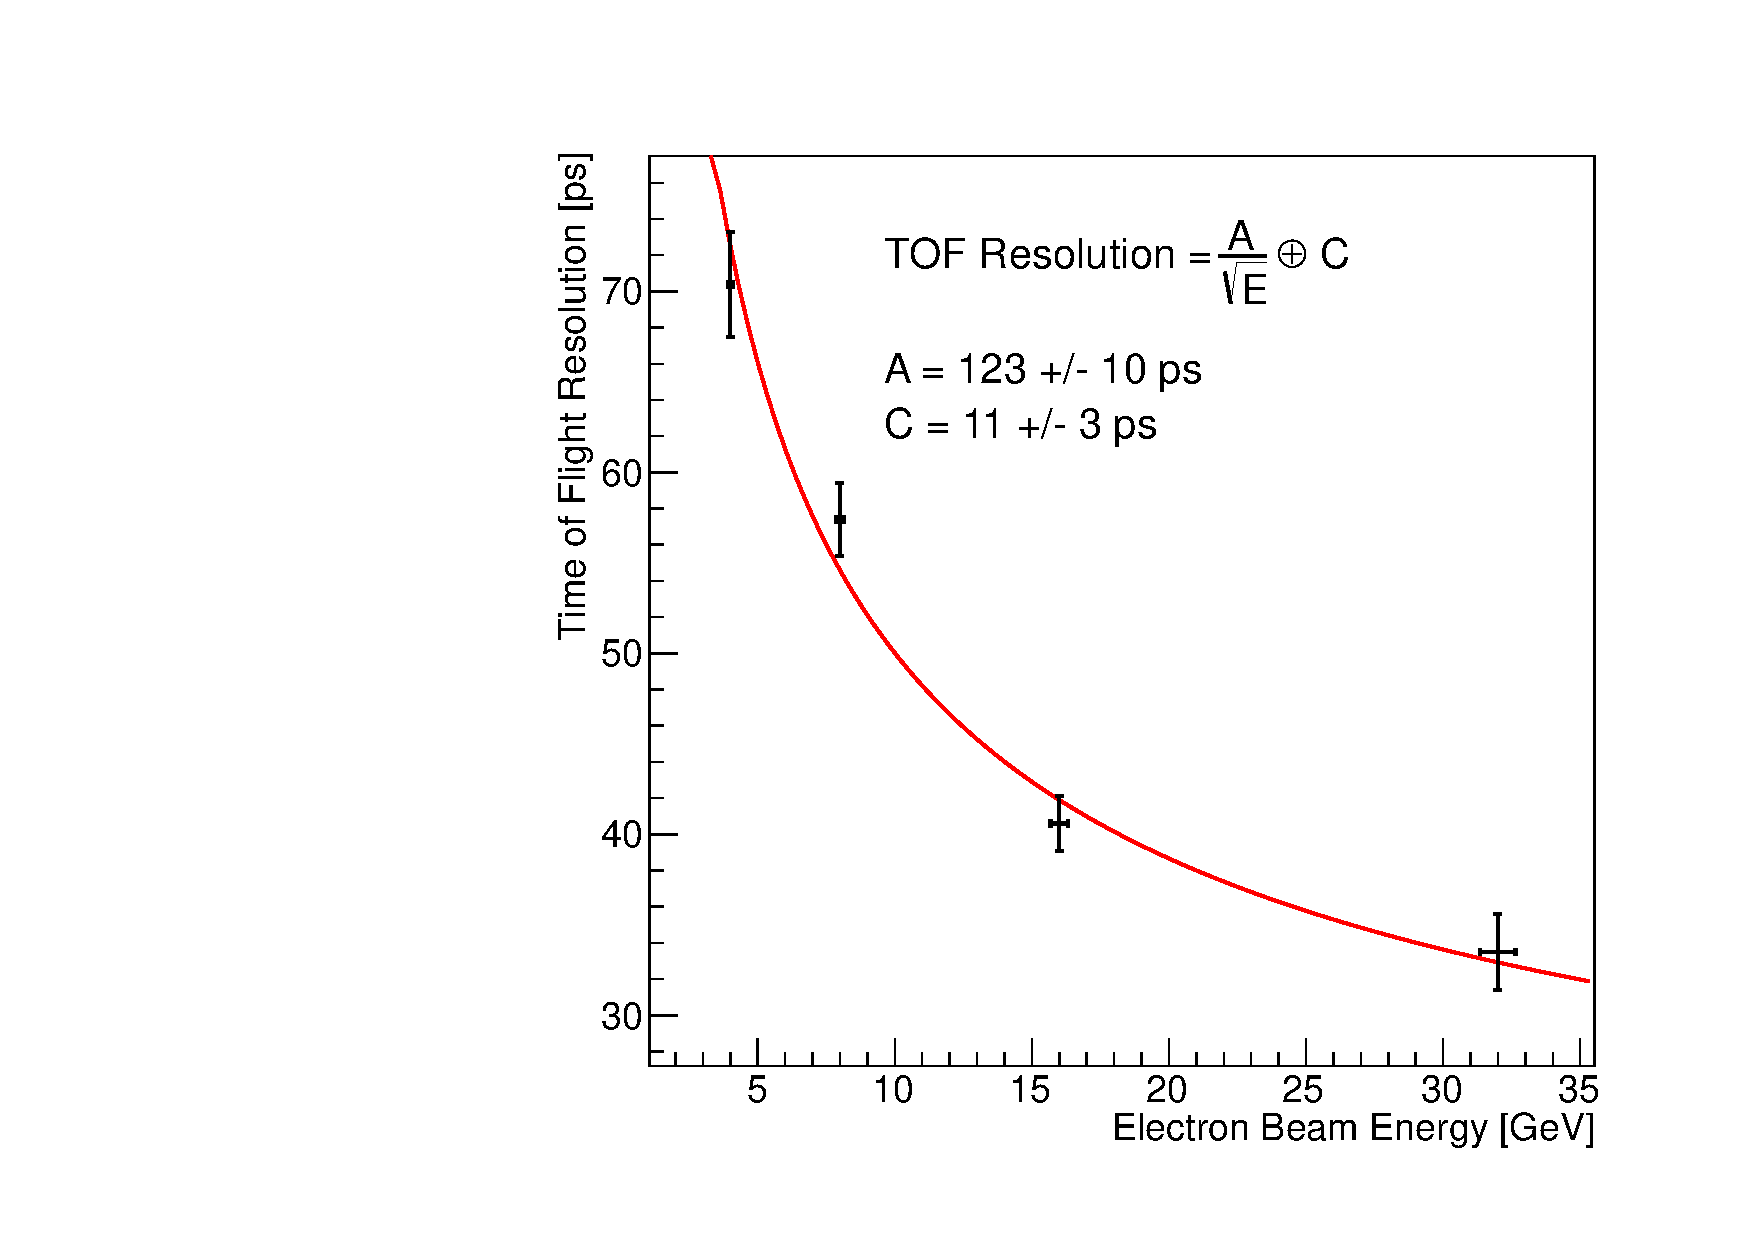
\includegraphics[width=0.45\textwidth]{figs/TimeResolutionVsEnergy_CrystalCube} 
\caption{ The time resolution measured using the LYSO cube
sampling calorimeter is plotted as a function of the electron beam energy, 
and fitted to the sum of a $1/\sqrt{E}$ term and a constant term. Note that the energy absorbed in the LYSO cube is a small fraction of the incident electron energy.}
\label{fig:LYSOCubeTOFResolutionVsEnergy}
\end{figure}

Given that we measure the contribution to the time resolution of the
photodetector and the DAQ electronics to be about $20$~ps, using the results from
the 32 GeV electron beam, we infer that the
combined contribution to the time resolution from the shower profile
fluctuations, the scintillation mechanism, and the optical transit inside the
LYSO cube is below $27$~ps. In future studies, we intend to further separate these
effects, in order to better isolate the impact of each of these components.

\subsection{Timing Studies of the LYSO-Tungsten Shashlik Calorimeter}

We study the time resolution of a LYSO-tungsten Shashlik calorimeter, one of the
proposed choices for the Phase 2 upgrade of the CMS endcap calorimeter
system~\cite{Contardo:1605208}. We compare the time resolution performance for
two alternative optical transport schemes. 

We begin with a scheme where scintillation light is collected by WLS fibers that
pass through a set of four holes in the LYSO and tungsten layers. In 
Figure~\ref{fig:ShashlikDiagram}, a shashlik cell and the light extraction 
scheme is illustrated. A schematic diagram and a photograph showing this experimental
setup are shown in Figure~\ref{fig:ShashlikFiberSetup}. MCP-PMT's produced by 
Hamamatsu (R3809) are used to collect the scintillation light, while a Photek 240 
MCP-PMT is used as a reference time detector. 

\begin{figure}[H] \centering
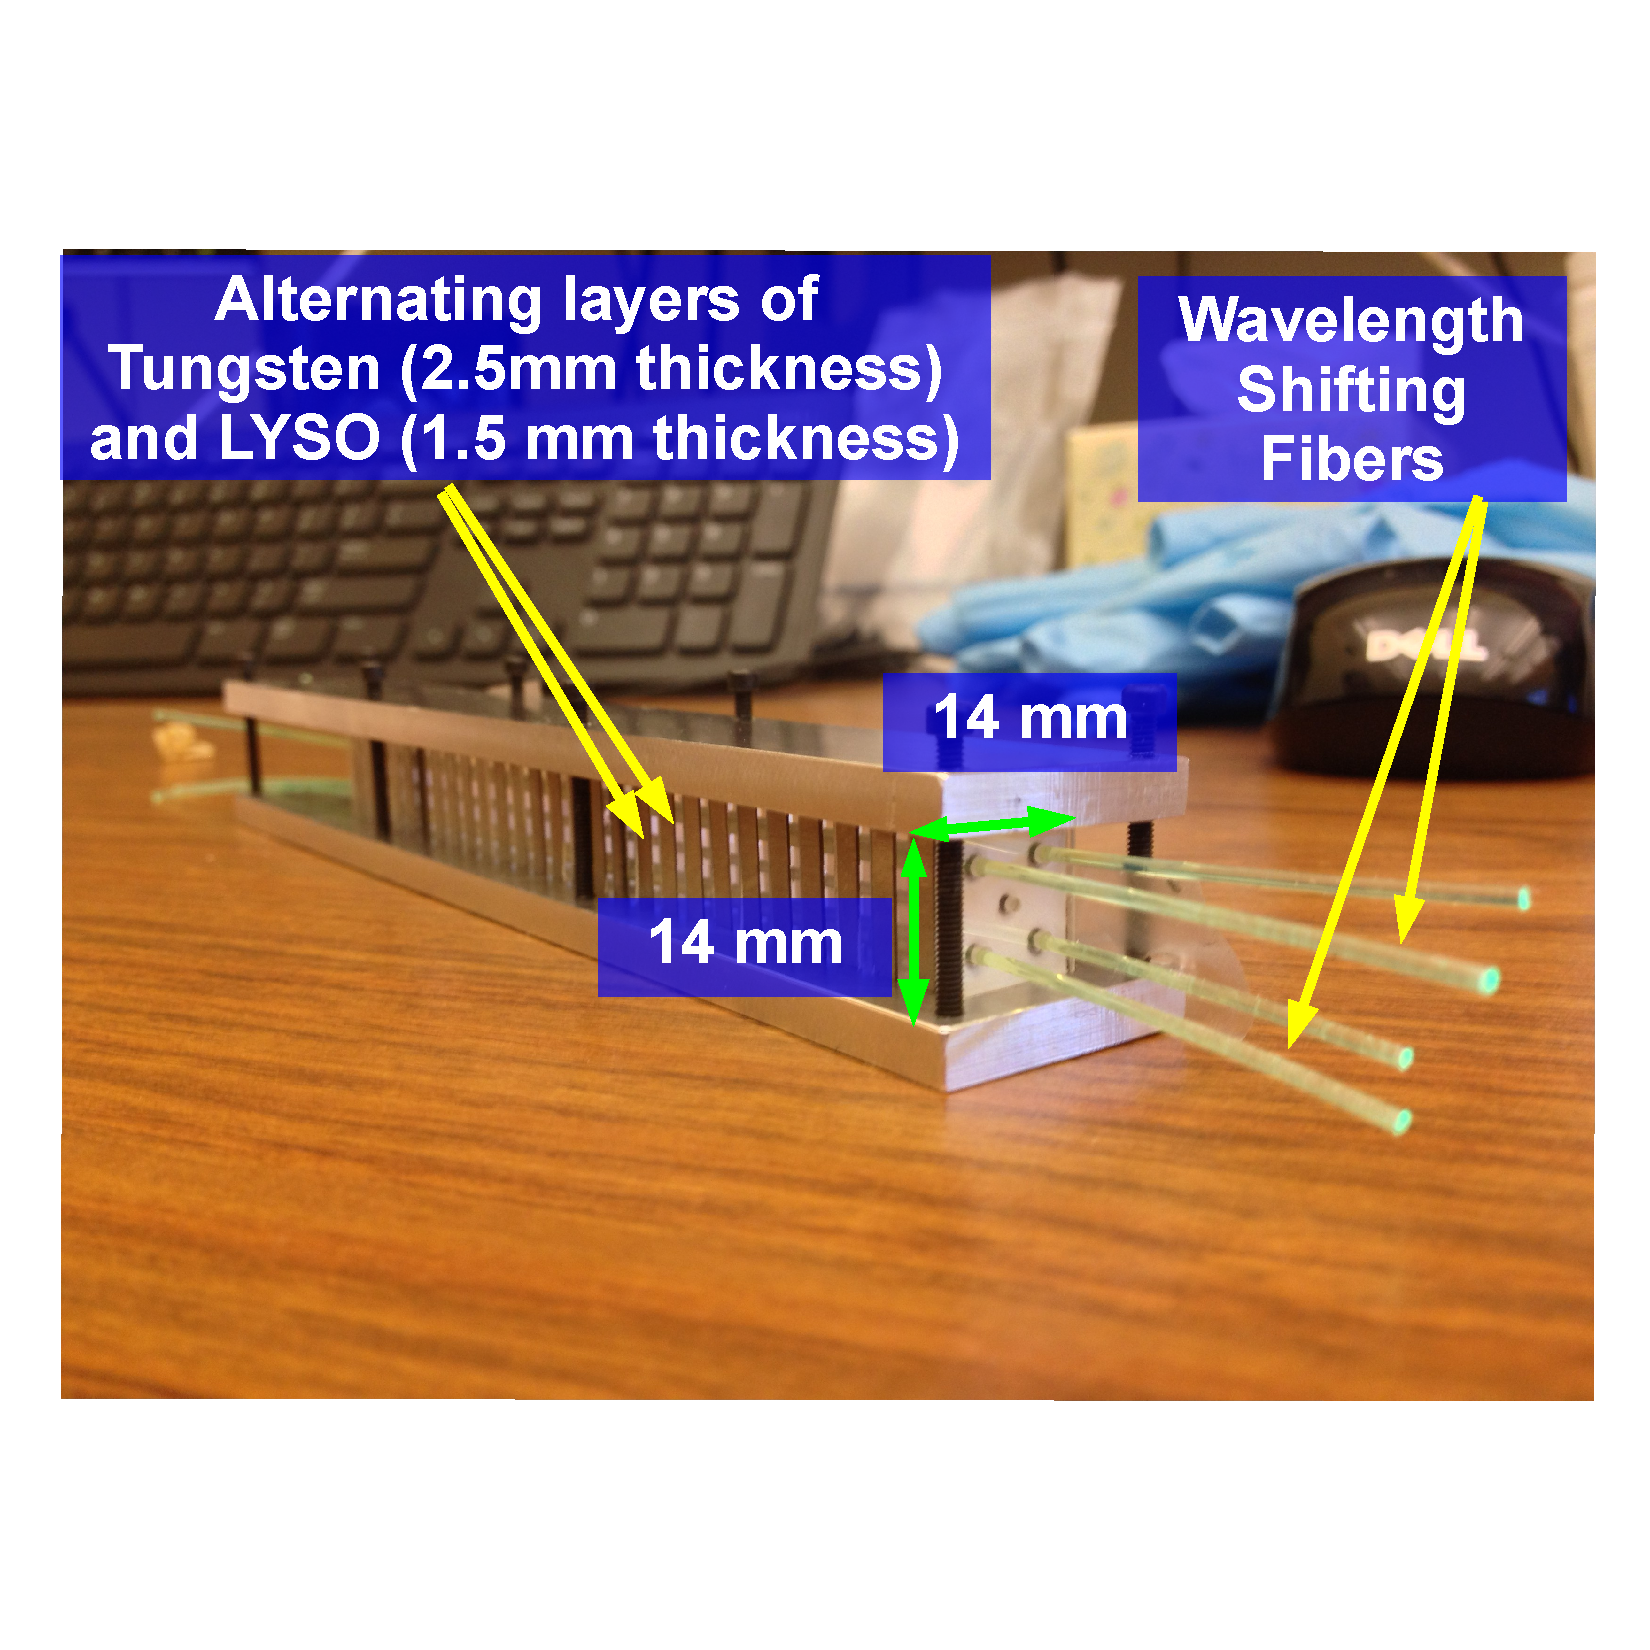
\includegraphics[width=0.6\textwidth]{figs/ShashlikCellPhoto.pdf} 
\caption{ The shashlik configuration based upon interleaved W and LYSO layers. 
Twenty-eight LYSO crystals and twenty-seven W plates comprise the module.
Four WLS fibers are used to read out the scintillation light from the 
tiles. } 
\label{fig:ShashlikDiagram}
\end{figure}

\begin{figure}[H] \centering
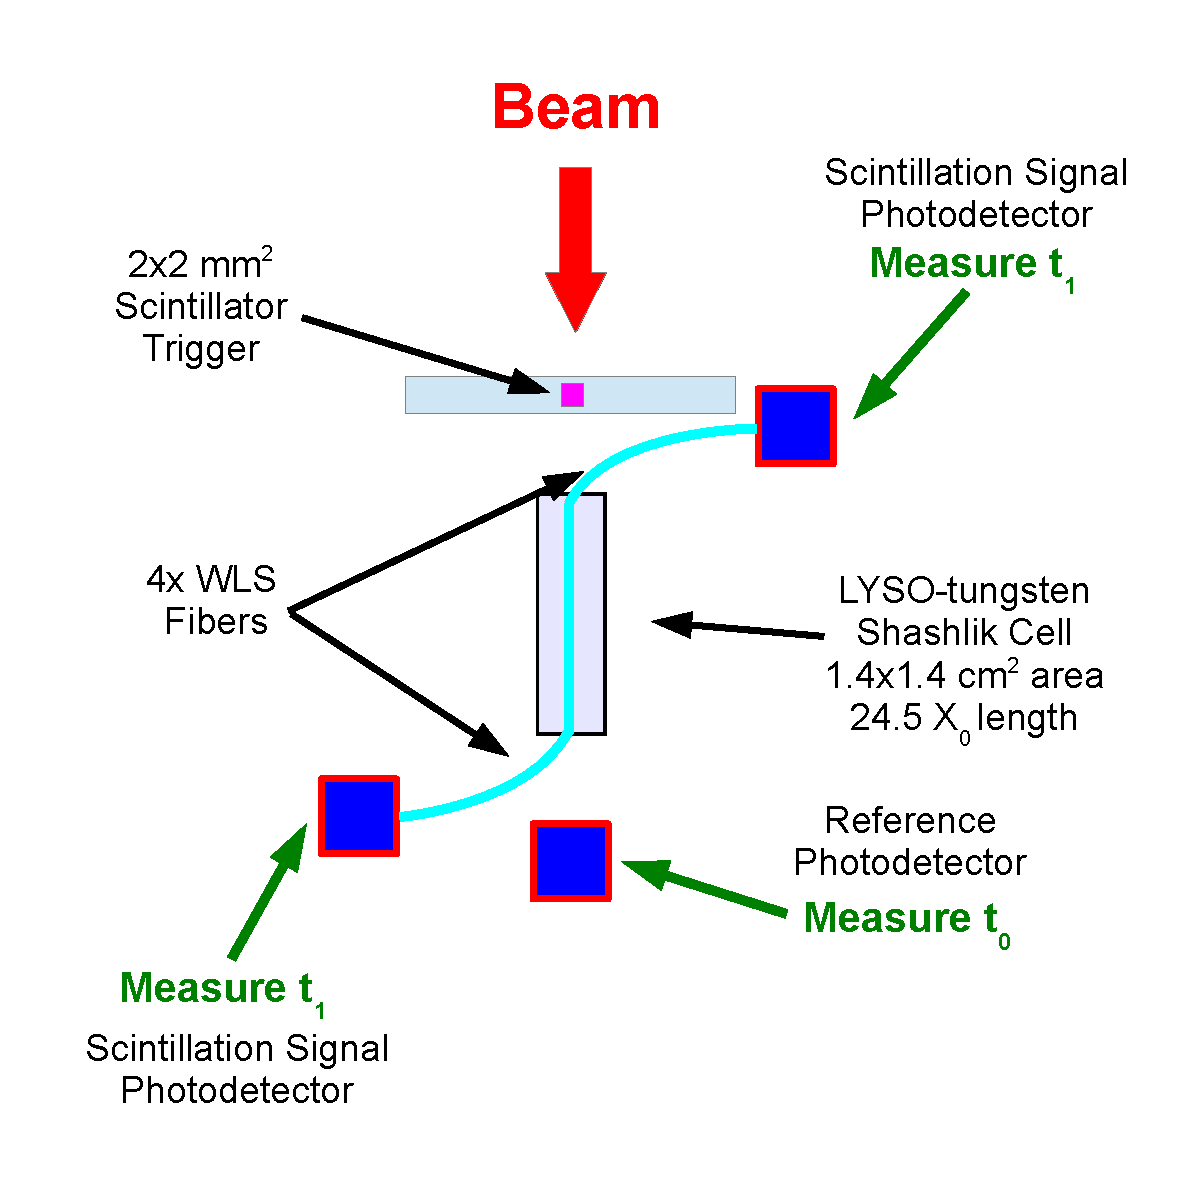
\includegraphics[width=0.45\textwidth]{figs/ShashlikFiberSetupSchematic} 
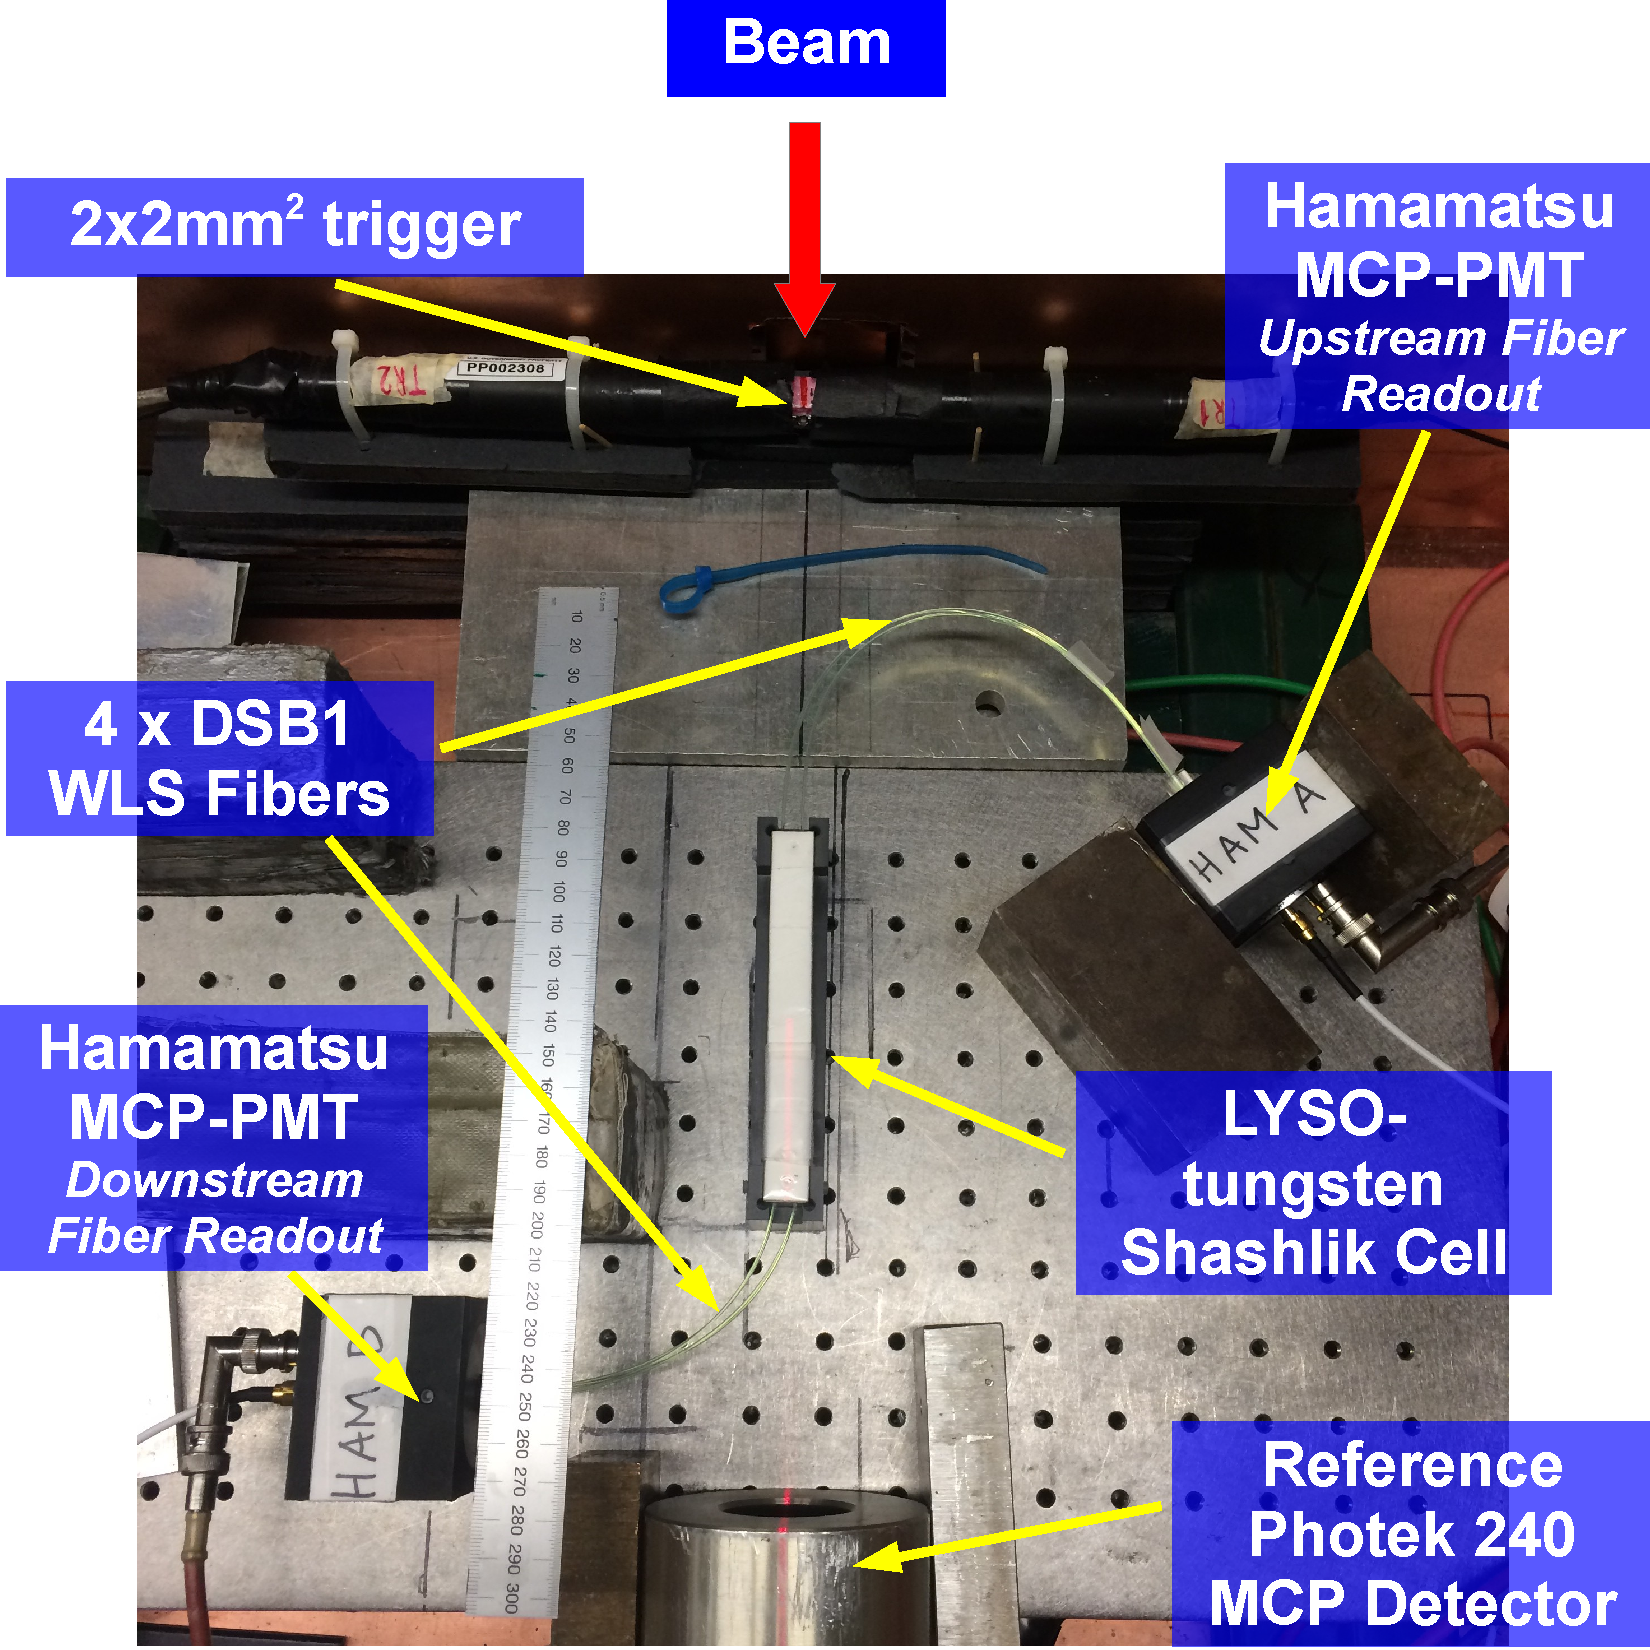
\includegraphics[width=0.45\textwidth]{figs/ShashlikFiberSetupPhoto} 
\caption{ A schematic diagram of the experimental setup for the
time of flight measurement using the LYSO-tungsten shashlik calorimeter
with fiber signal extraction, along with a photograph of the
experimental setup. } 
\label{fig:ShashlikFiberSetup}
\end{figure}

In this setup the wavelength shifting mechanism in the fibers affects the rise
time and time jitter of the final signal pulse. We investigate this effect in
greater detail by comparing the signal pulses obtained using two different types
of WLS fiber in the same LYSO-tungsten shashlik calorimeter. In
Figure~\ref{fig:FiberPulseComparison} we show the pulse shapes averaged over a
few hundred events obtained using DSB1 fibers~\cite{Albrecht} and Y11 fibers,
plotted in blue and red respectively, compared with the average pulse shape
obtained from direct optical coupling of the photodector to the edge of one of
the LYSO tiles, plotted in green. We find that the rise time of the pulse
obtained using the DSB1 fibers, about $2.4$~ns, is significantly faster than the
rise time of the pulse obtained using the Y11 fibers, which is about $7.1$~ns.
This indicates that the choice of fiber is an important parameter for optimizing
the time resolution of this type of calorimeter, and that the DSB1 fiber
provides a reasonably good choice. Furthermore, we note that these signal rise
times are comparable to the measured decay times of the corresponding WLS
fibers~\cite{Albrecht}.

\begin{figure}[H] \centering
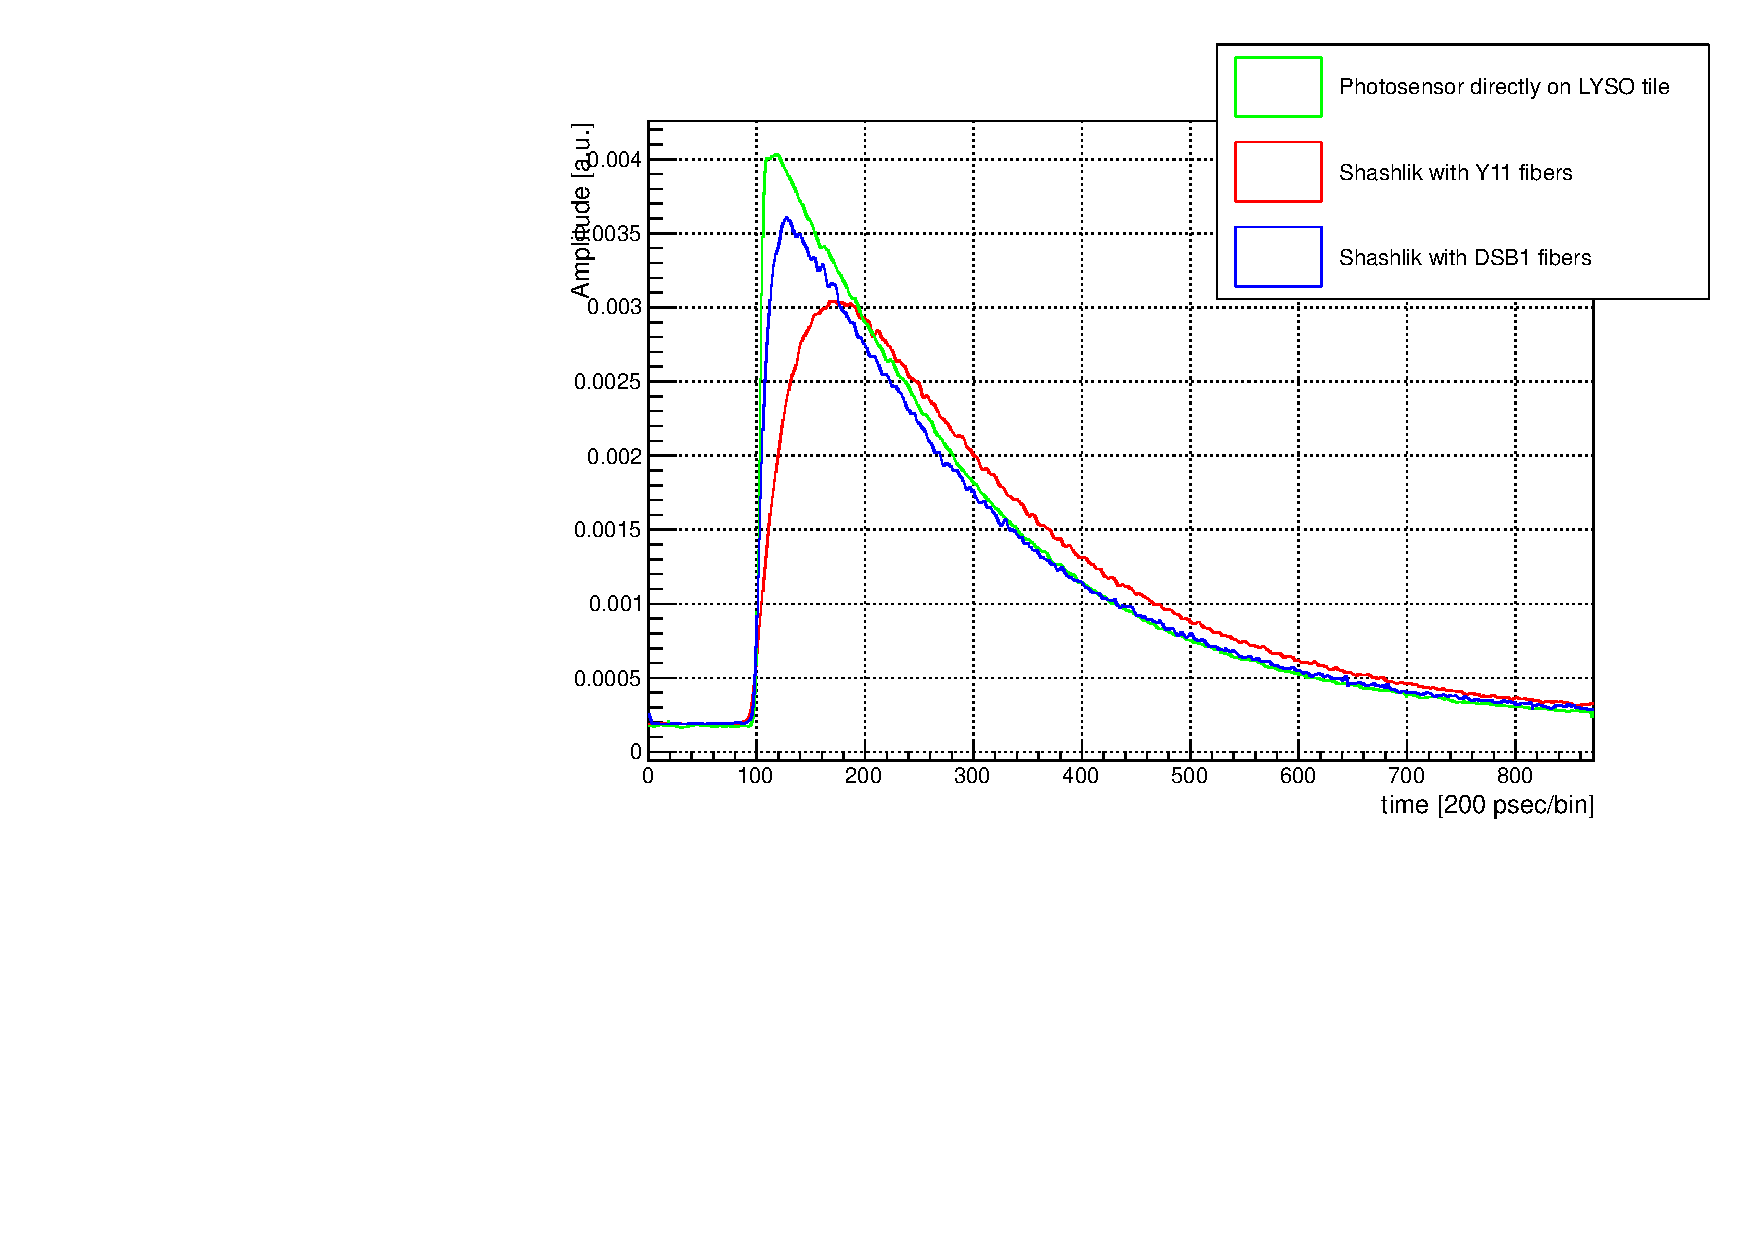
\includegraphics[width=0.45\textwidth]{figs/FiberPulses} 
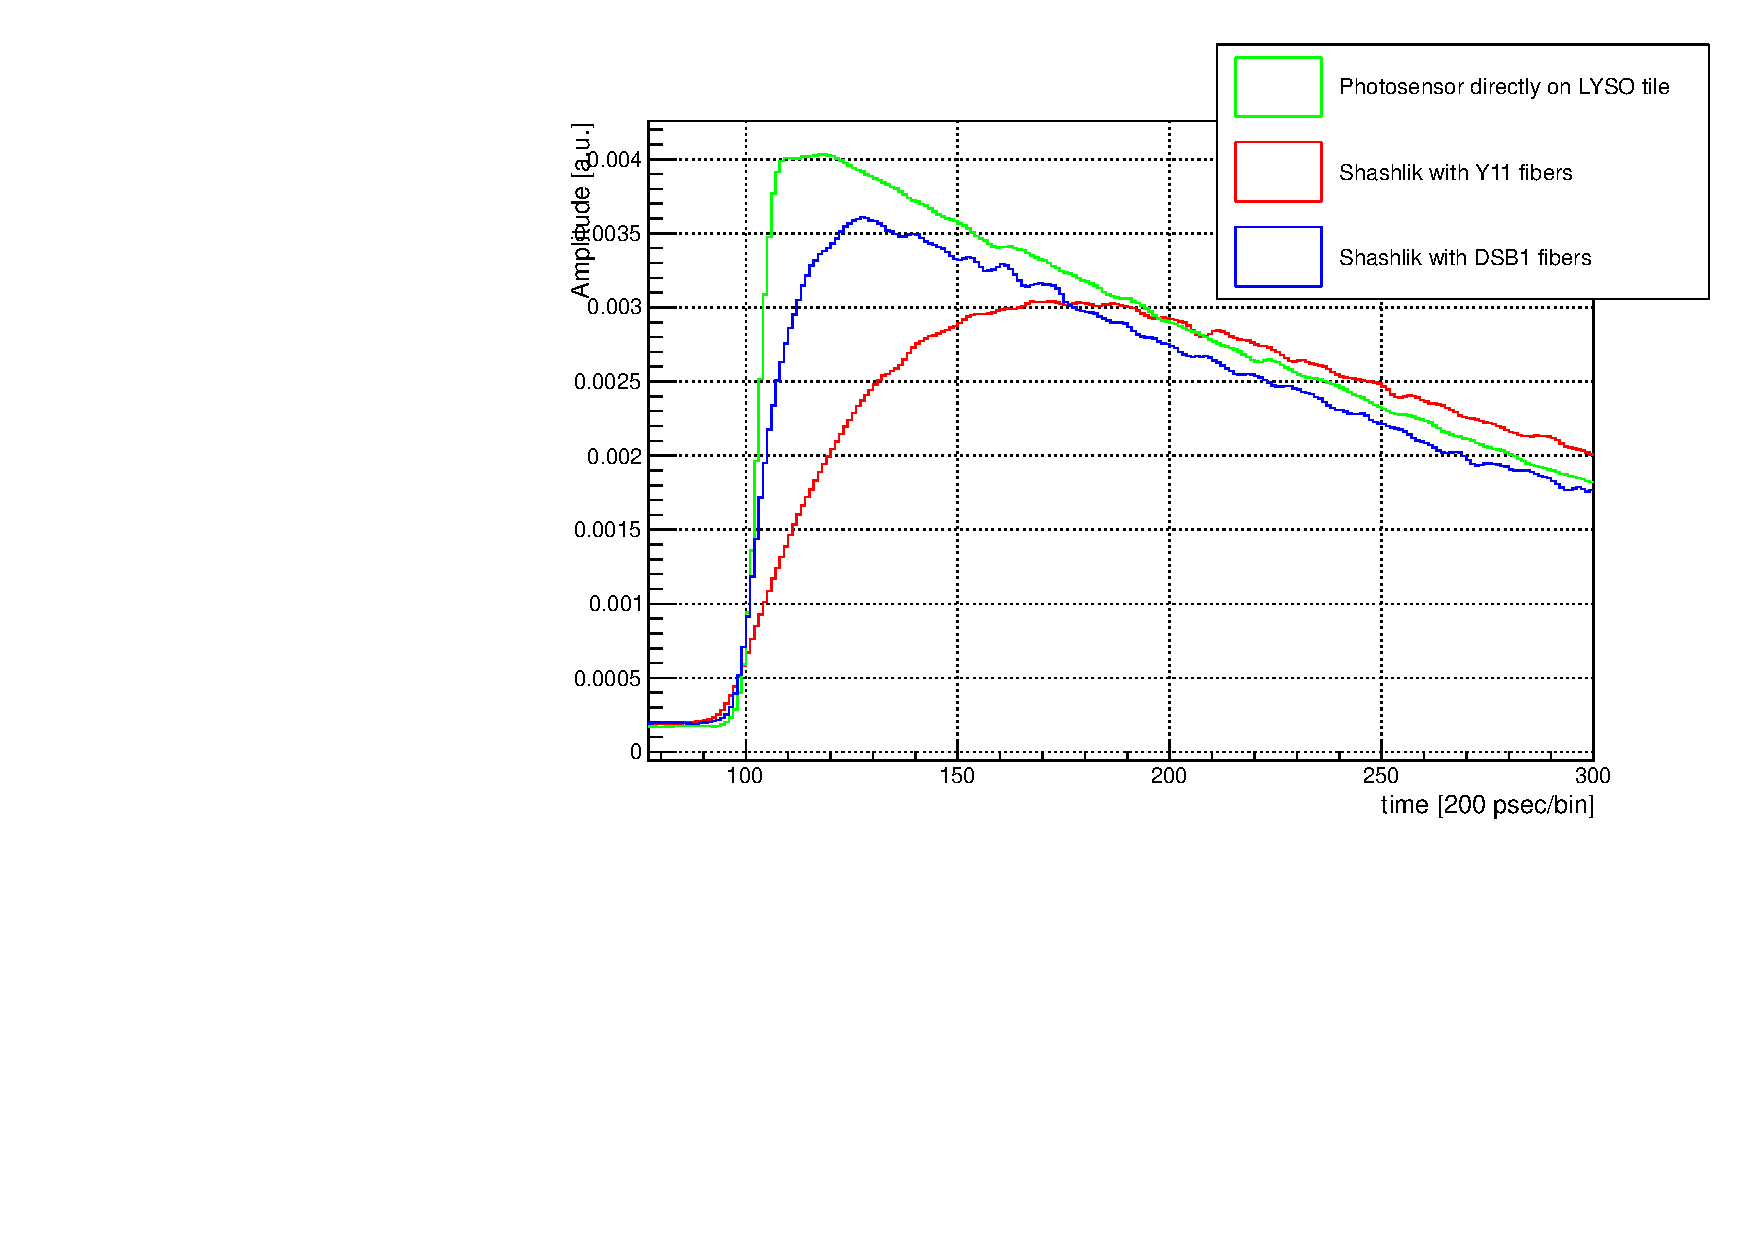
\includegraphics[width=0.45\textwidth]{figs/FiberPulsesZoom} 
\caption{(Left) Pulse shapes digitized by the DRS4 board and averaged over several hundred events 
obtained from the LYSO-tungsten shashlik calorimeter with light extracted using
DSB1 (blue) and Y11 (red) WLS fibers, are compared with 
the averaged pulse shapes obtained from direct coupling of the photodetector (green)
to one edge of one of the LYSO tiles in the shashlik calorimeter. (Right) A zoomed-in version of the figure on the left.} 
\label{fig:FiberPulseComparison}
\end{figure}


Using the shashlik calorimeter cell with DSB1 fibers, we measure the time resolution
for electron beams with energy varying between $4$~GeV and $32$~GeV.
In Figure~\ref{fig:ShashlikFiberEnergy32GeV} we show the distribution
of the pulse integral, a quantity proportional to the total collected charge,
for the $32$~GeV beam, and observe an energy resolution of about $5\%$.
Time of flight distributions, fitted to gaussian functions,
are shown in Figure~\ref{fig:ShashlikFiberTOF}, and the 
$\sigma$ parameter of the gaussian fit is plotted as a function of the
beam energy in Figure~\ref{fig:ShashlikFiberTOFResolutionVsEnergy}.
We find that the dependence of the time resolution on
beam energy follows a $1/\sqrt{E}$ functional form, indicating
that the current calorimeter setup remains in the photostatistics
limited regime. The best time resolution we obtain
with this setup is $104$~ps. As the measurements are photostatistics
limited, the result can be improved in the future if the light collection
efficiency is increased.

\begin{figure}[H] \centering
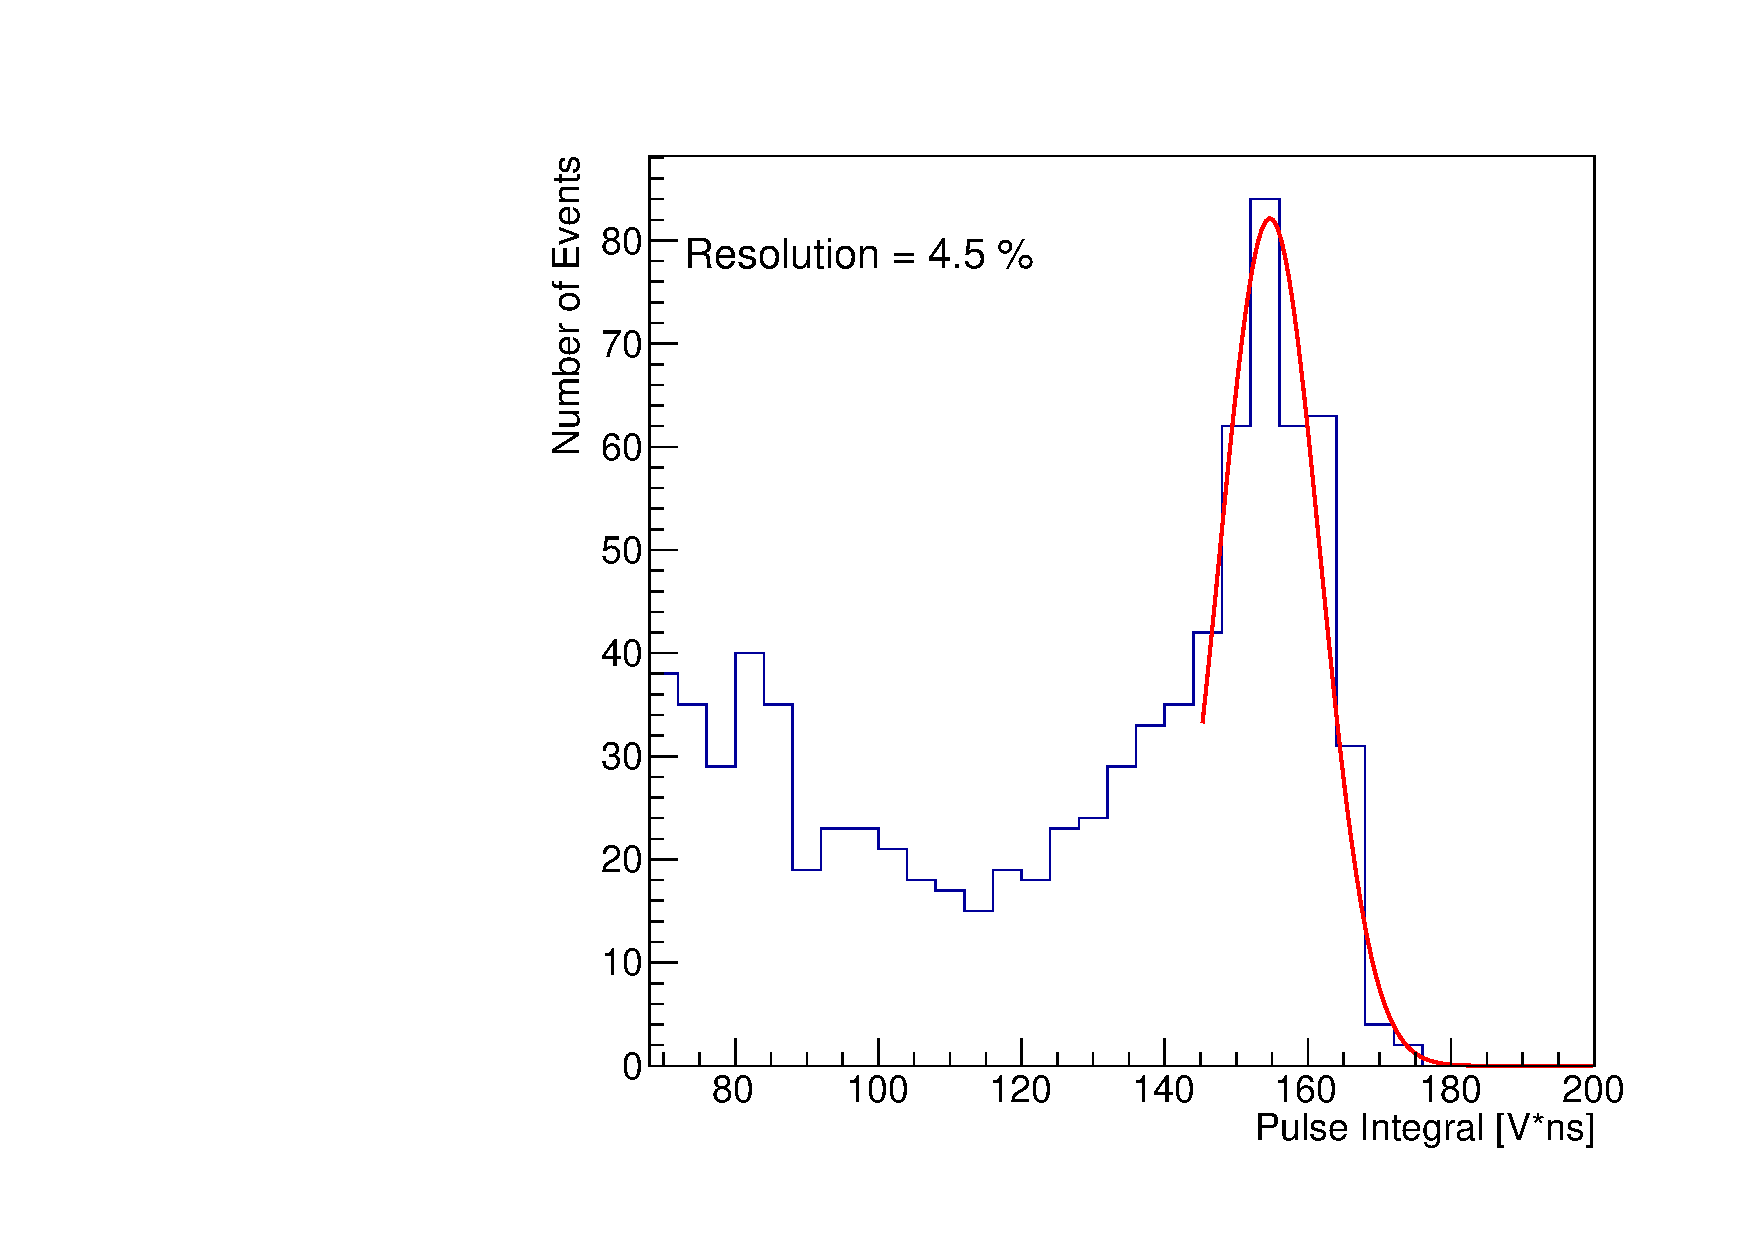
\includegraphics[width=0.45\textwidth]{figs/TOF_ShashlikDSB1Fiber_Electron_32GeV_energy} 
\caption{ Histogram of the pulse integral for events recorded using
the LYSO-tungsten shashlik calorimeter using DSB1 fibers, for 
a $32$~GeV electron beam. No electron identification requirements
are made in this run due to a misconfiguration of the Cherenkov counter,
so background is visible in the spectrum. } 
\label{fig:ShashlikFiberEnergy32GeV}
\end{figure}

\begin{figure}[H] \centering
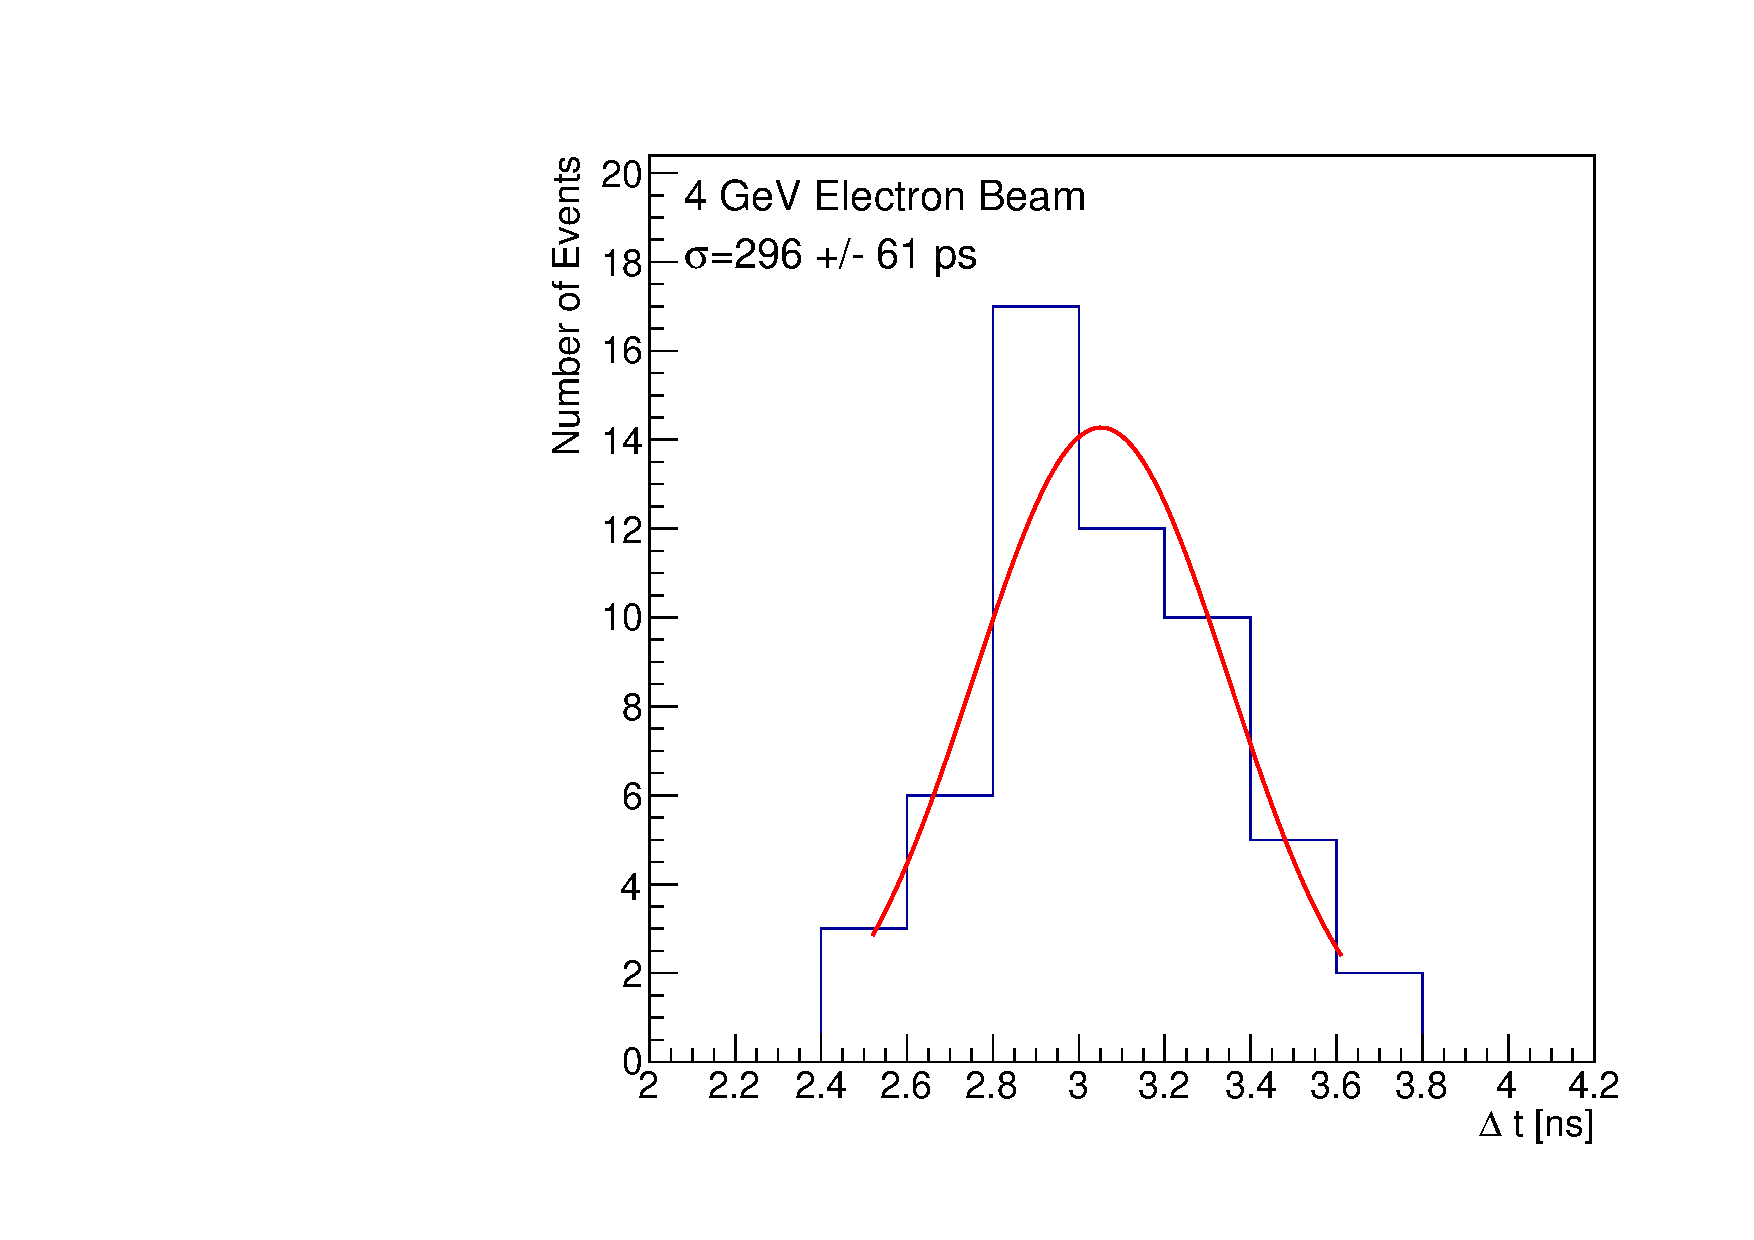
\includegraphics[width=0.45\textwidth]{figs/TOF_ShashlikDSB1Fiber_Electron_4GeV} 
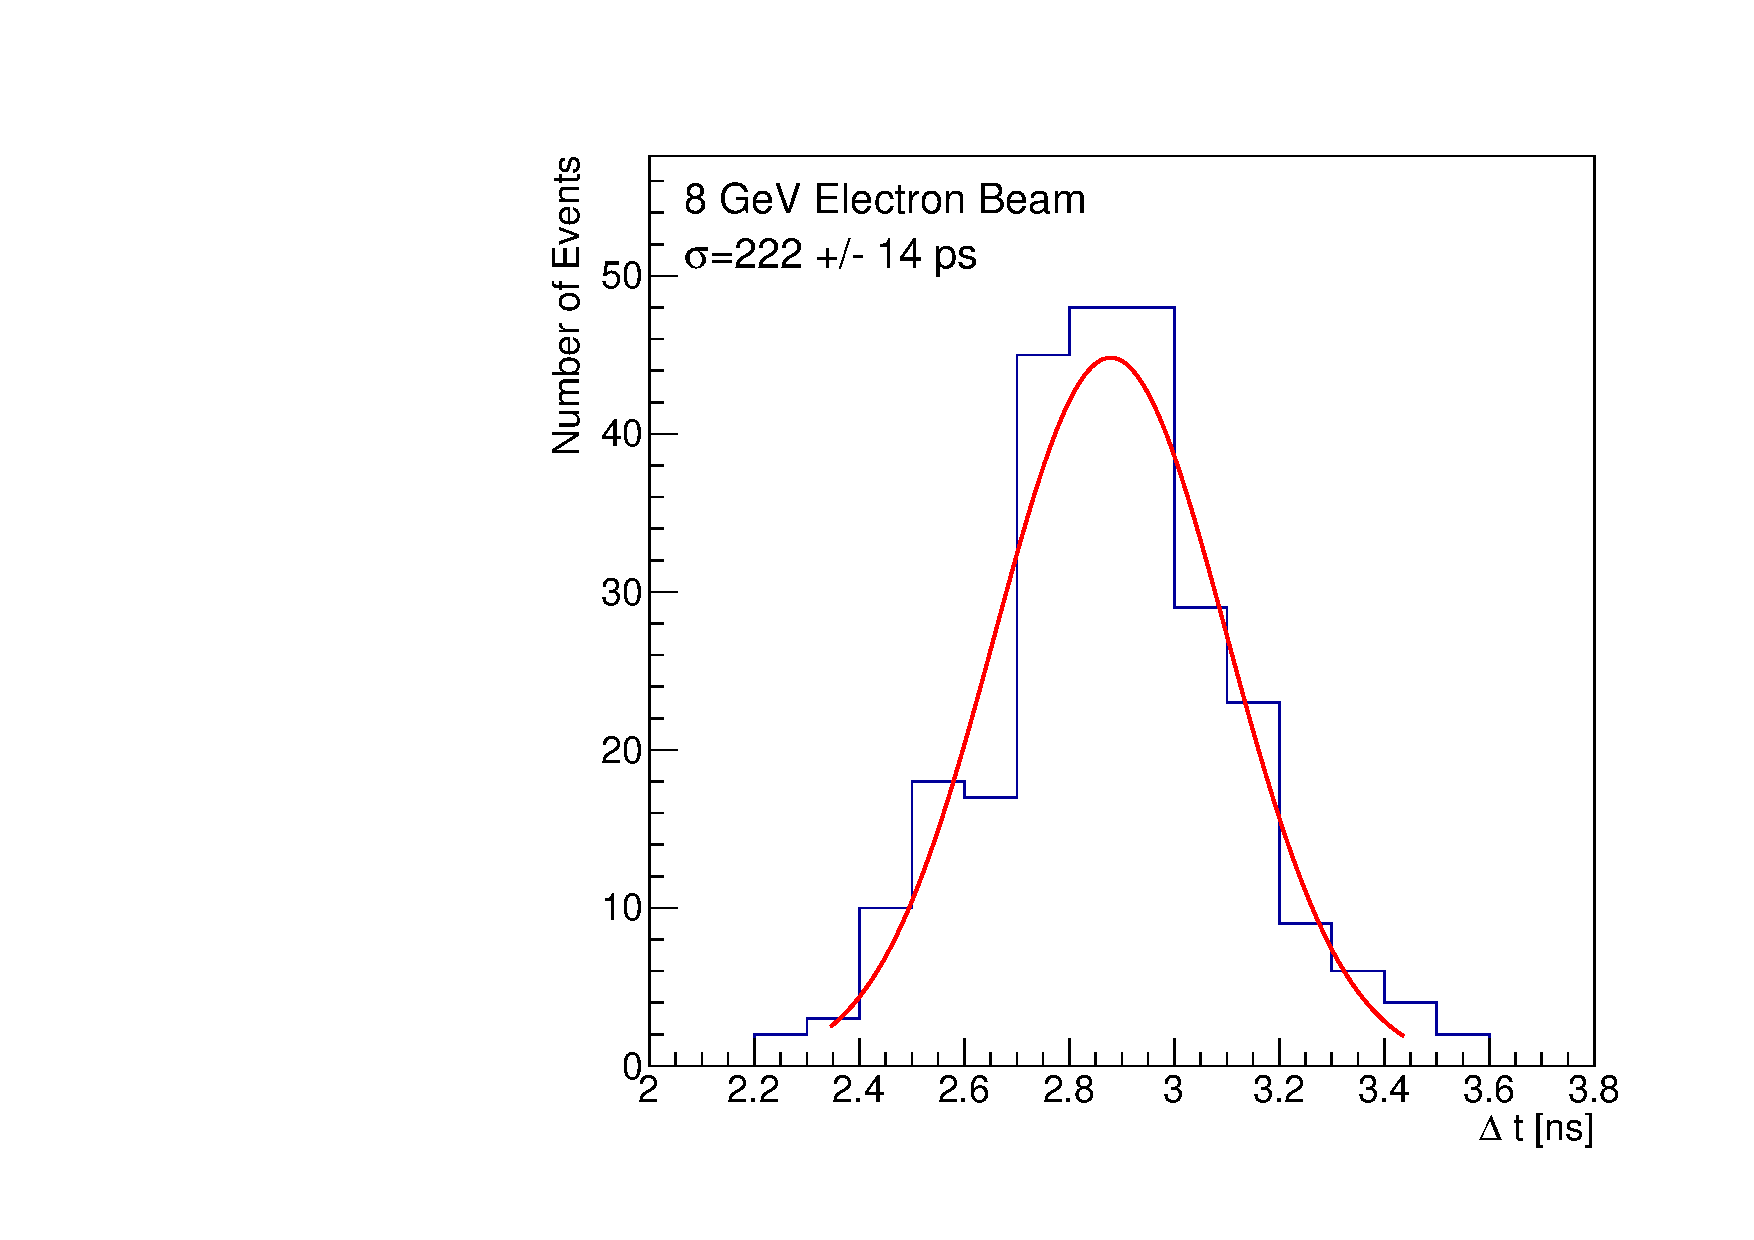
\includegraphics[width=0.45\textwidth]{figs/TOF_ShashlikDSB1Fiber_Electron_8GeV} 
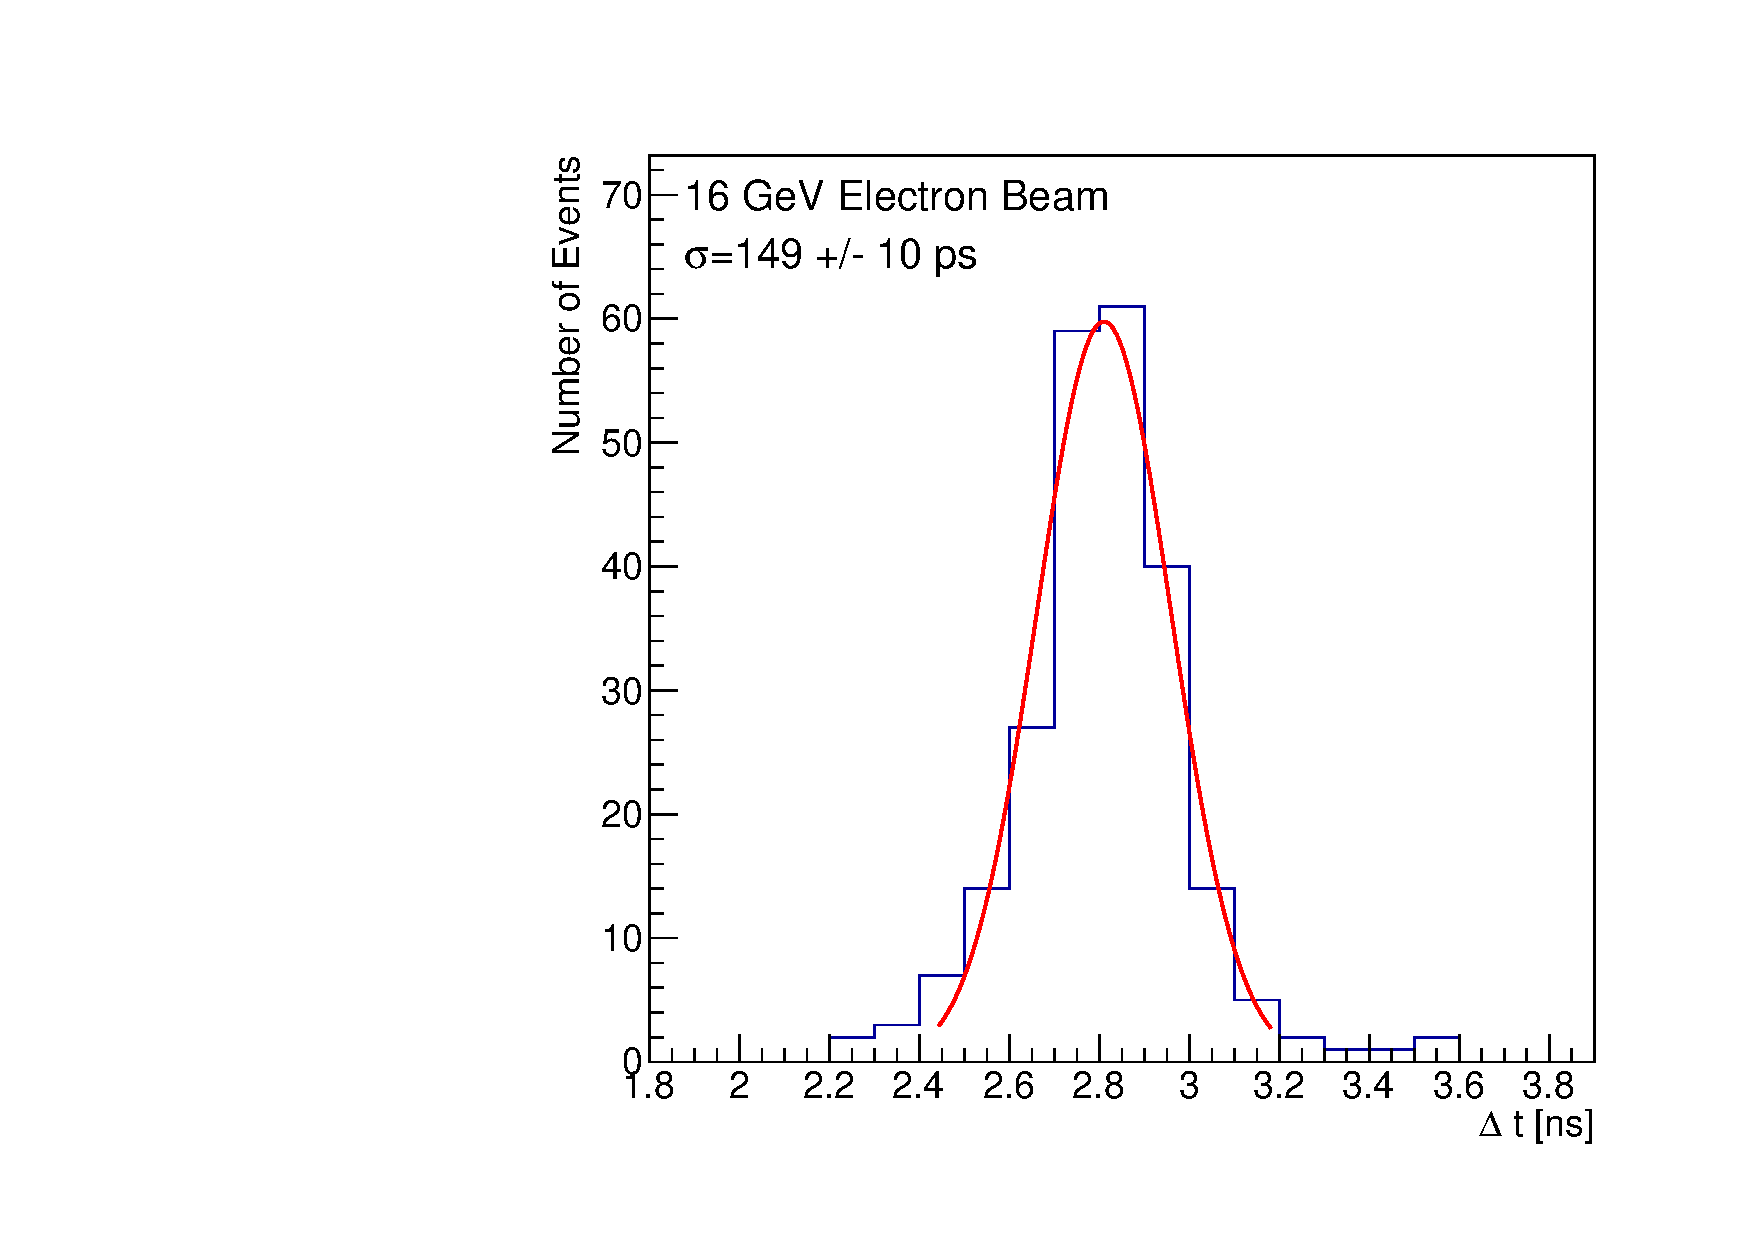
\includegraphics[width=0.45\textwidth]{figs/TOF_ShashlikDSB1Fiber_Electron_16GeV} 
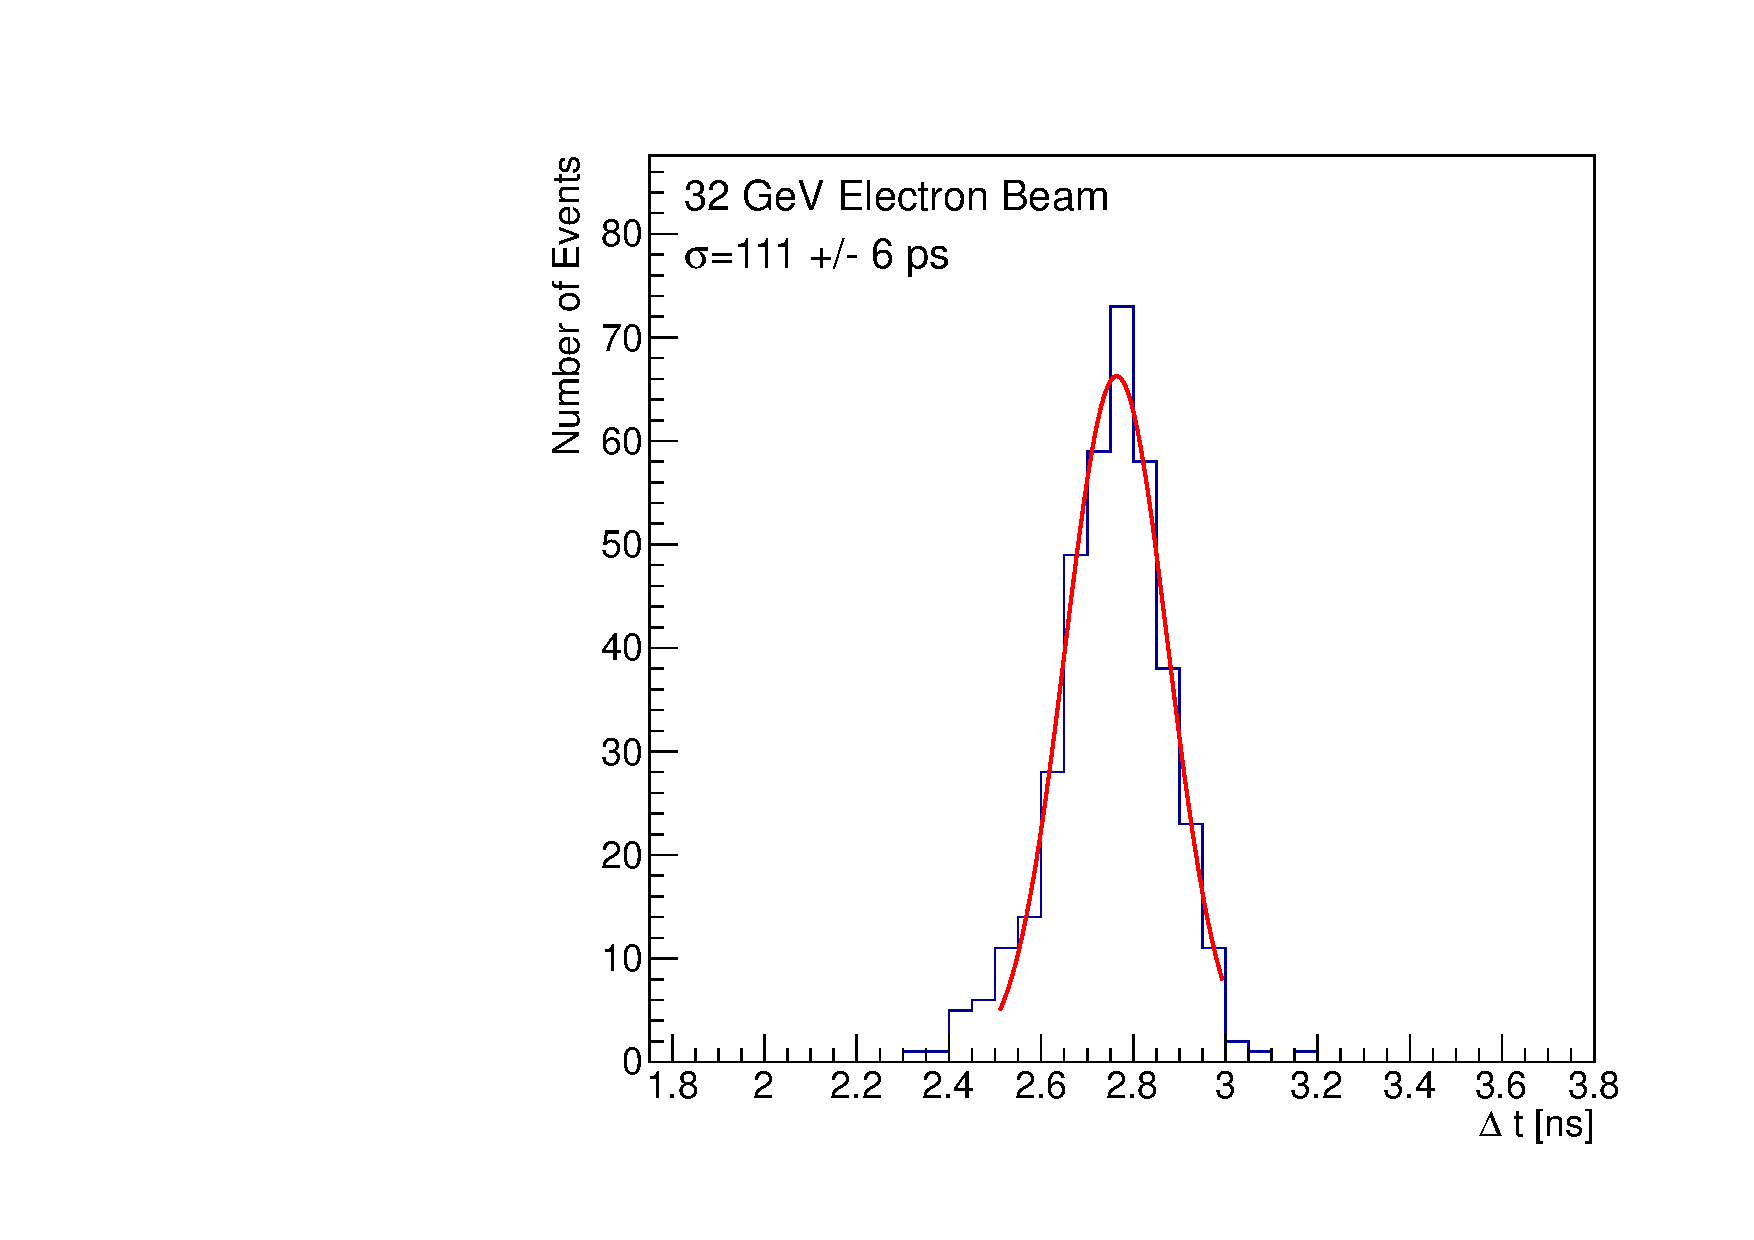
\includegraphics[width=0.45\textwidth]{figs/TOF_ShashlikDSB1Fiber_Electron_32GeV} 
\caption{ Time of flight distributions for the LYSO-tungsten shashlik calorimeter
using DSB1 fibers for electron beams with varying beam energies. } 
\label{fig:ShashlikFiberTOF}
\end{figure}

\begin{figure}[H] \centering
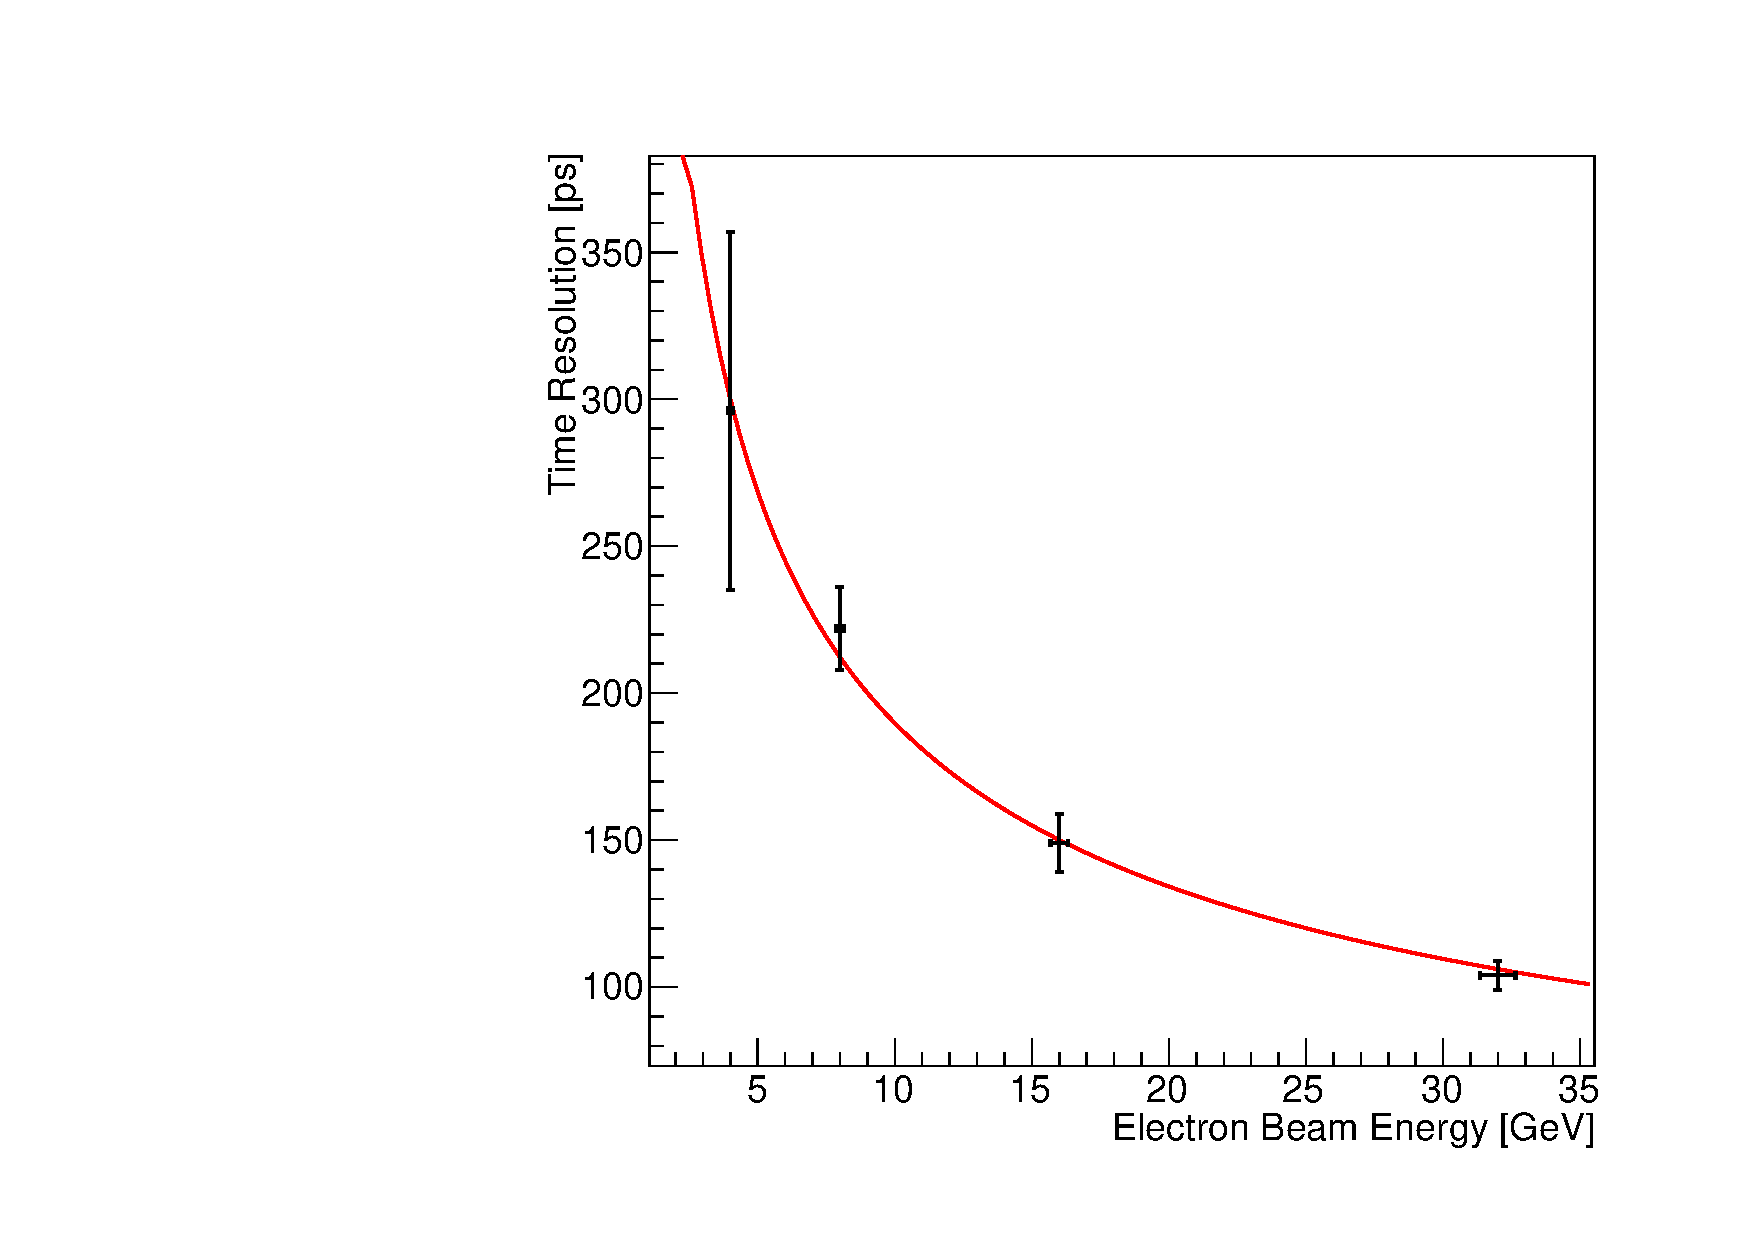
\includegraphics[width=0.45\textwidth]{figs/TimeResolutionVsEnergy_ShashlikDSB1Fiber} 
\caption{ The time resolution measured using the LYSO-tungsten shashlik
calorimeter with signal extracted using DSB1 fibers is plotted as a function of
the electron beam energy, and fitted to a $1/\sqrt{E}$ functional form. }
\label{fig:ShashlikFiberTOFResolutionVsEnergy}
\end{figure}


Next, we studied an alternative scheme in which the MCP-PMT photodetectors are
directly coupled to the edges of two adjacent LYSO layers in the shashlik
calorimeter and scintillation light is directly transported to the photodetector
through the edges of the tile layers. A schematic diagram and corresponding
photograph of the experimental setup are shown in
Figure~\ref{fig:ShashlikSideReadoutSetup}. In
Figure~\ref{fig:ShashlikSideReadoutExposedLayersPhoto}, we show a zoomed-in
photograph of the exposed LYSO layers from which the scintillation light signal
is extracted.

\begin{figure}[H] \centering
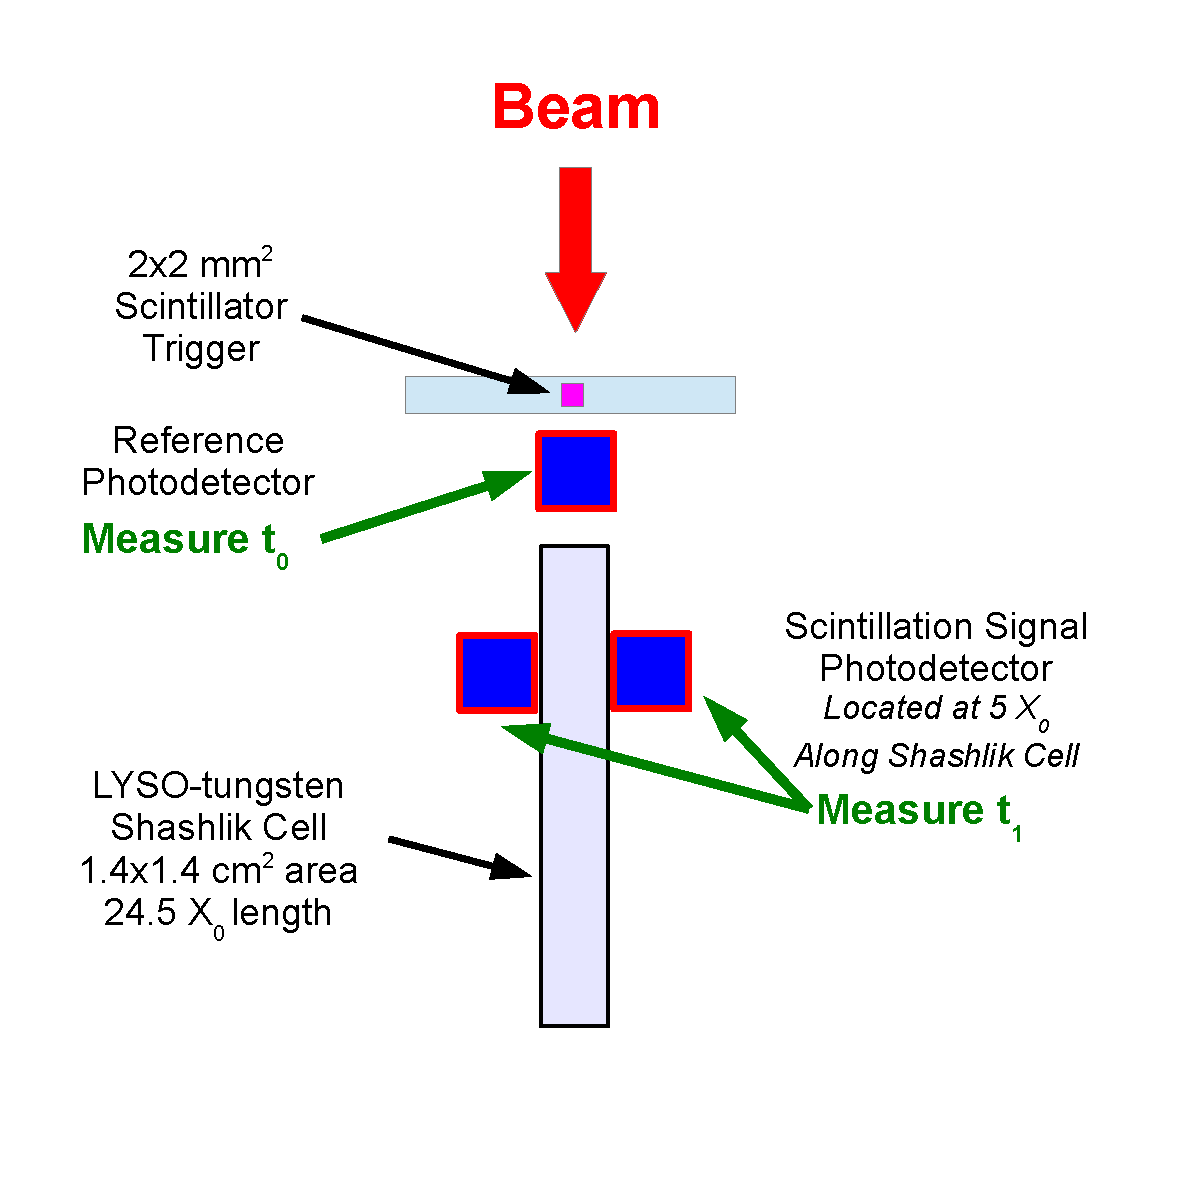
\includegraphics[width=0.45\textwidth]{figs/ShashlikSideReadoutSetupSchematic} 
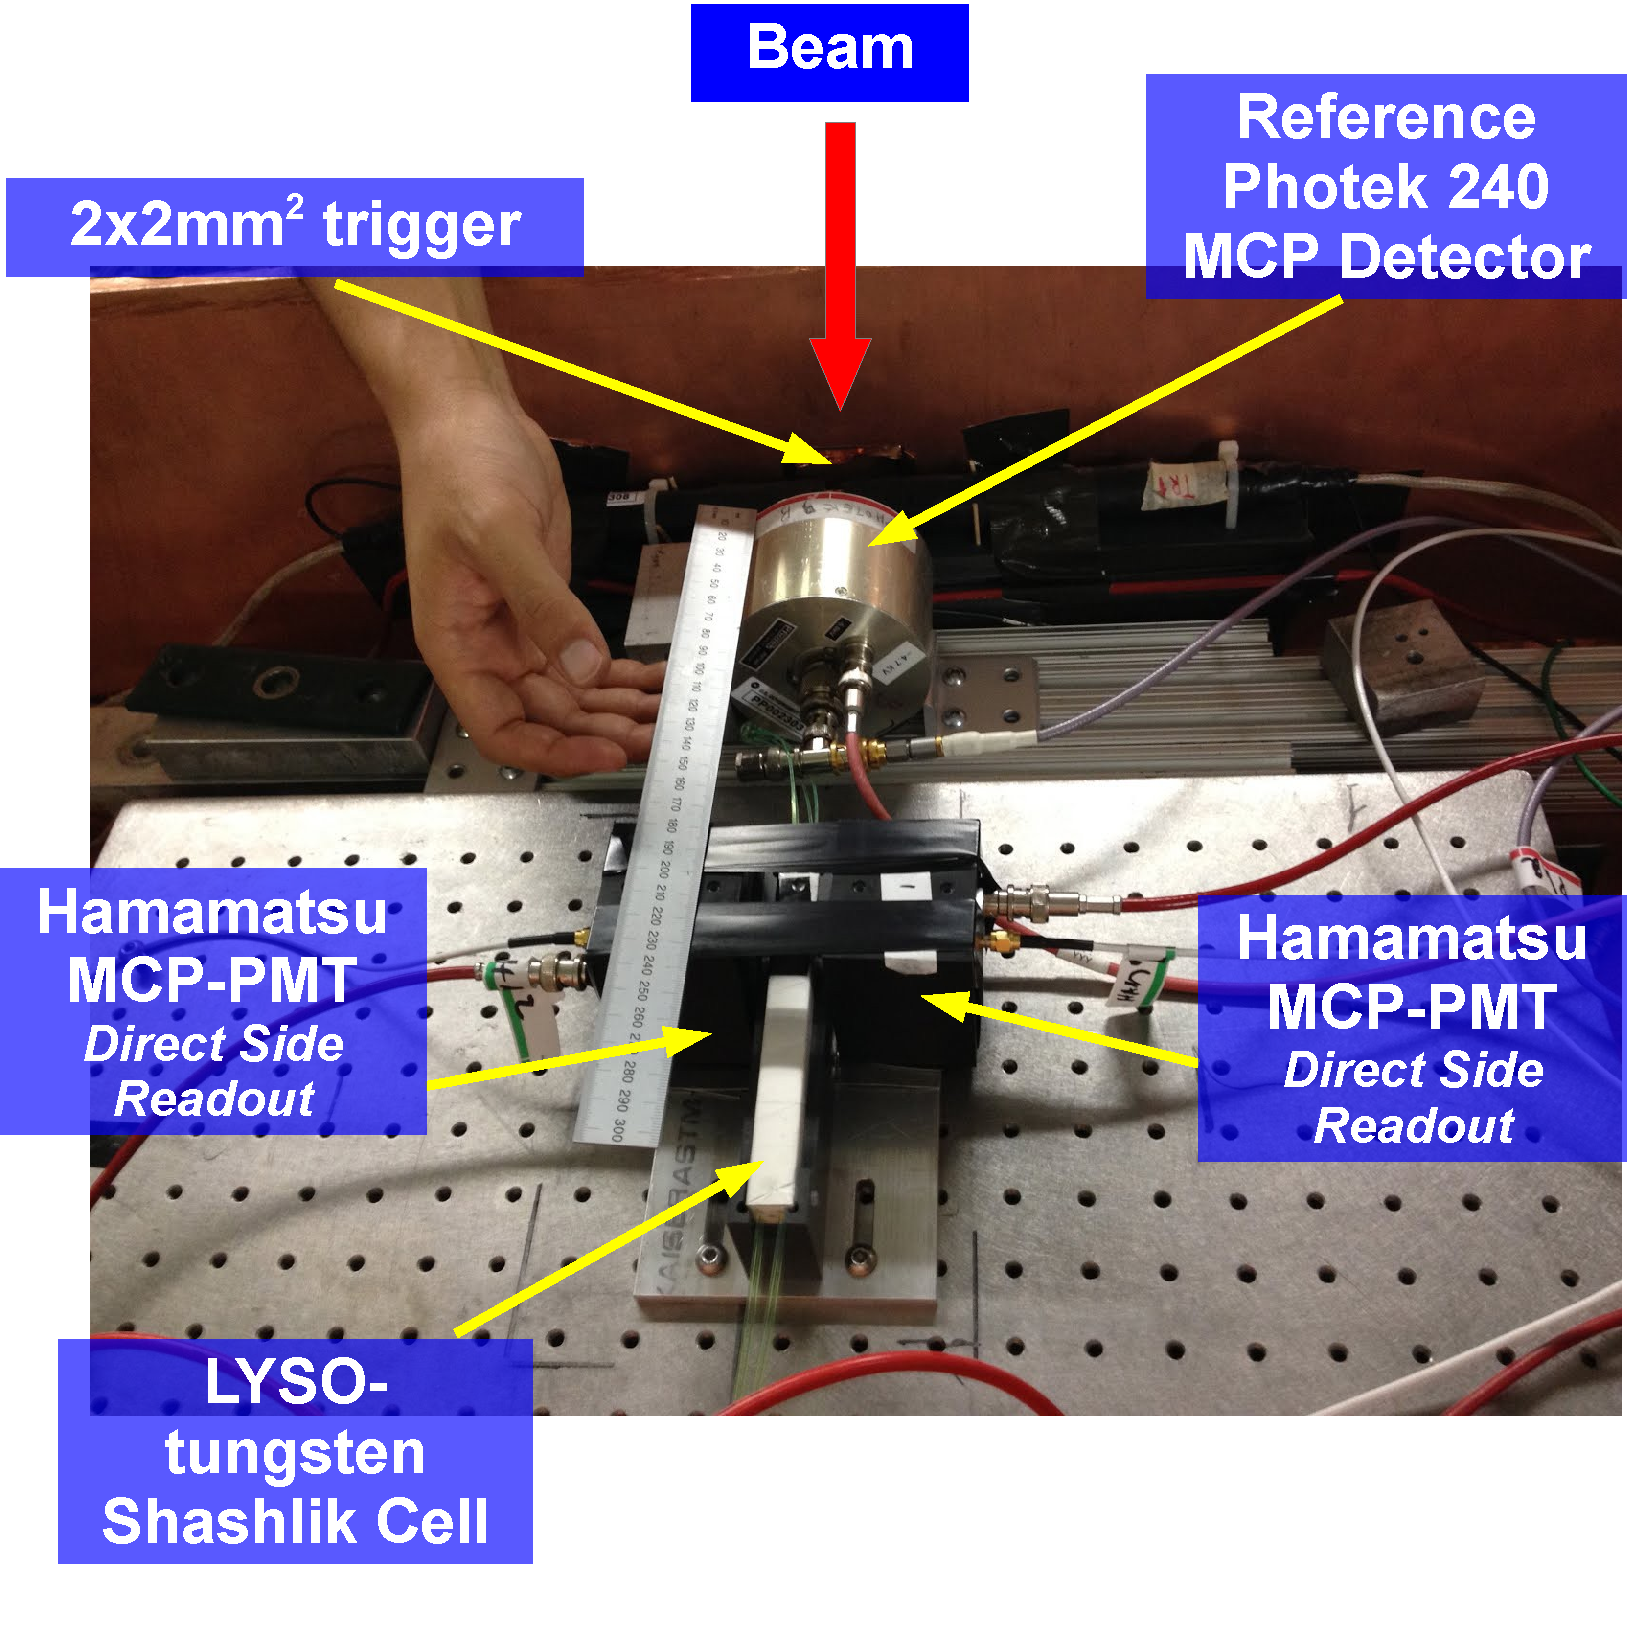
\includegraphics[width=0.45\textwidth]{figs/ShashlikSideReadoutPhotoB} 
\caption{ A schematic diagram of the experimental setup for the
time of flight measurement using the LYSO-tungsten shashlik calorimeter
with signal extraction from the edges of two LYSO layers, along
with a photograph of the experimental setup. } 
\label{fig:ShashlikSideReadoutSetup}
\end{figure}

\begin{figure}[H] \centering
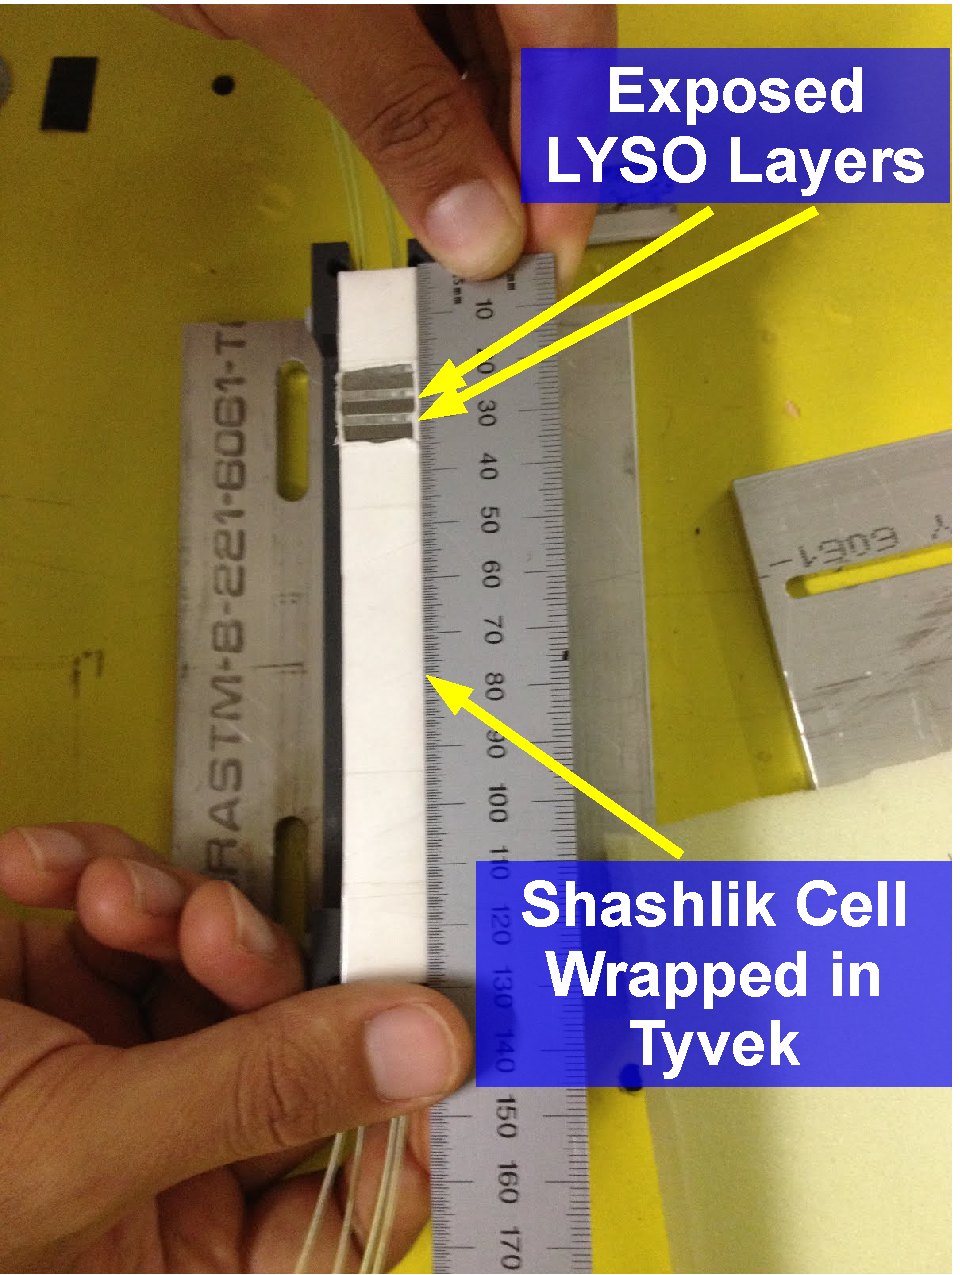
\includegraphics[width=0.30\textwidth]{figs/ShashlikSideReadoutPhotoA} 
\caption{ A photograph of the two exposed LYSO layers in the shashlik cell.
The scintillation light signal is extracted by optically coupling
the edges of these two exposed LYSO layers to MCP-PMT
photodetectors. } 
\label{fig:ShashlikSideReadoutExposedLayersPhoto}
\end{figure}


This setup allows us to study the relationship between the impact of the optical
transit time jitter and the impact of limited photostatistics. By placing the
photodetectors in direct contact with the edges of two LYSO layers, we minimize
the distance that scintillation light must travel to reach the photodetectors,
and thereby reduce the impact of optical transit on the time resolution. This
also reduces the available photostatistics, as we collect light from only a
small fraction of the shashlik cell. In Figure~\ref{fig:ShashlikSideReadoutTOF},
we show the time of flight distributions for electron beams at various energies,
fitted to gaussian functions. The width of the best-fit gaussian is plotted as a
function of the beam energy in
Figure~\ref{fig:ShashlikSideReadoutTOFResolutionVsEnergy}. The best time
resolution that we obtain is about $55$~ps, and fitting the result to the sum of
a $1/\sqrt{E}$ term and a constant term, we find a constant term of about
$30$~ps with a statistical uncertainty of $30\%$. 

\begin{figure}[H] \centering
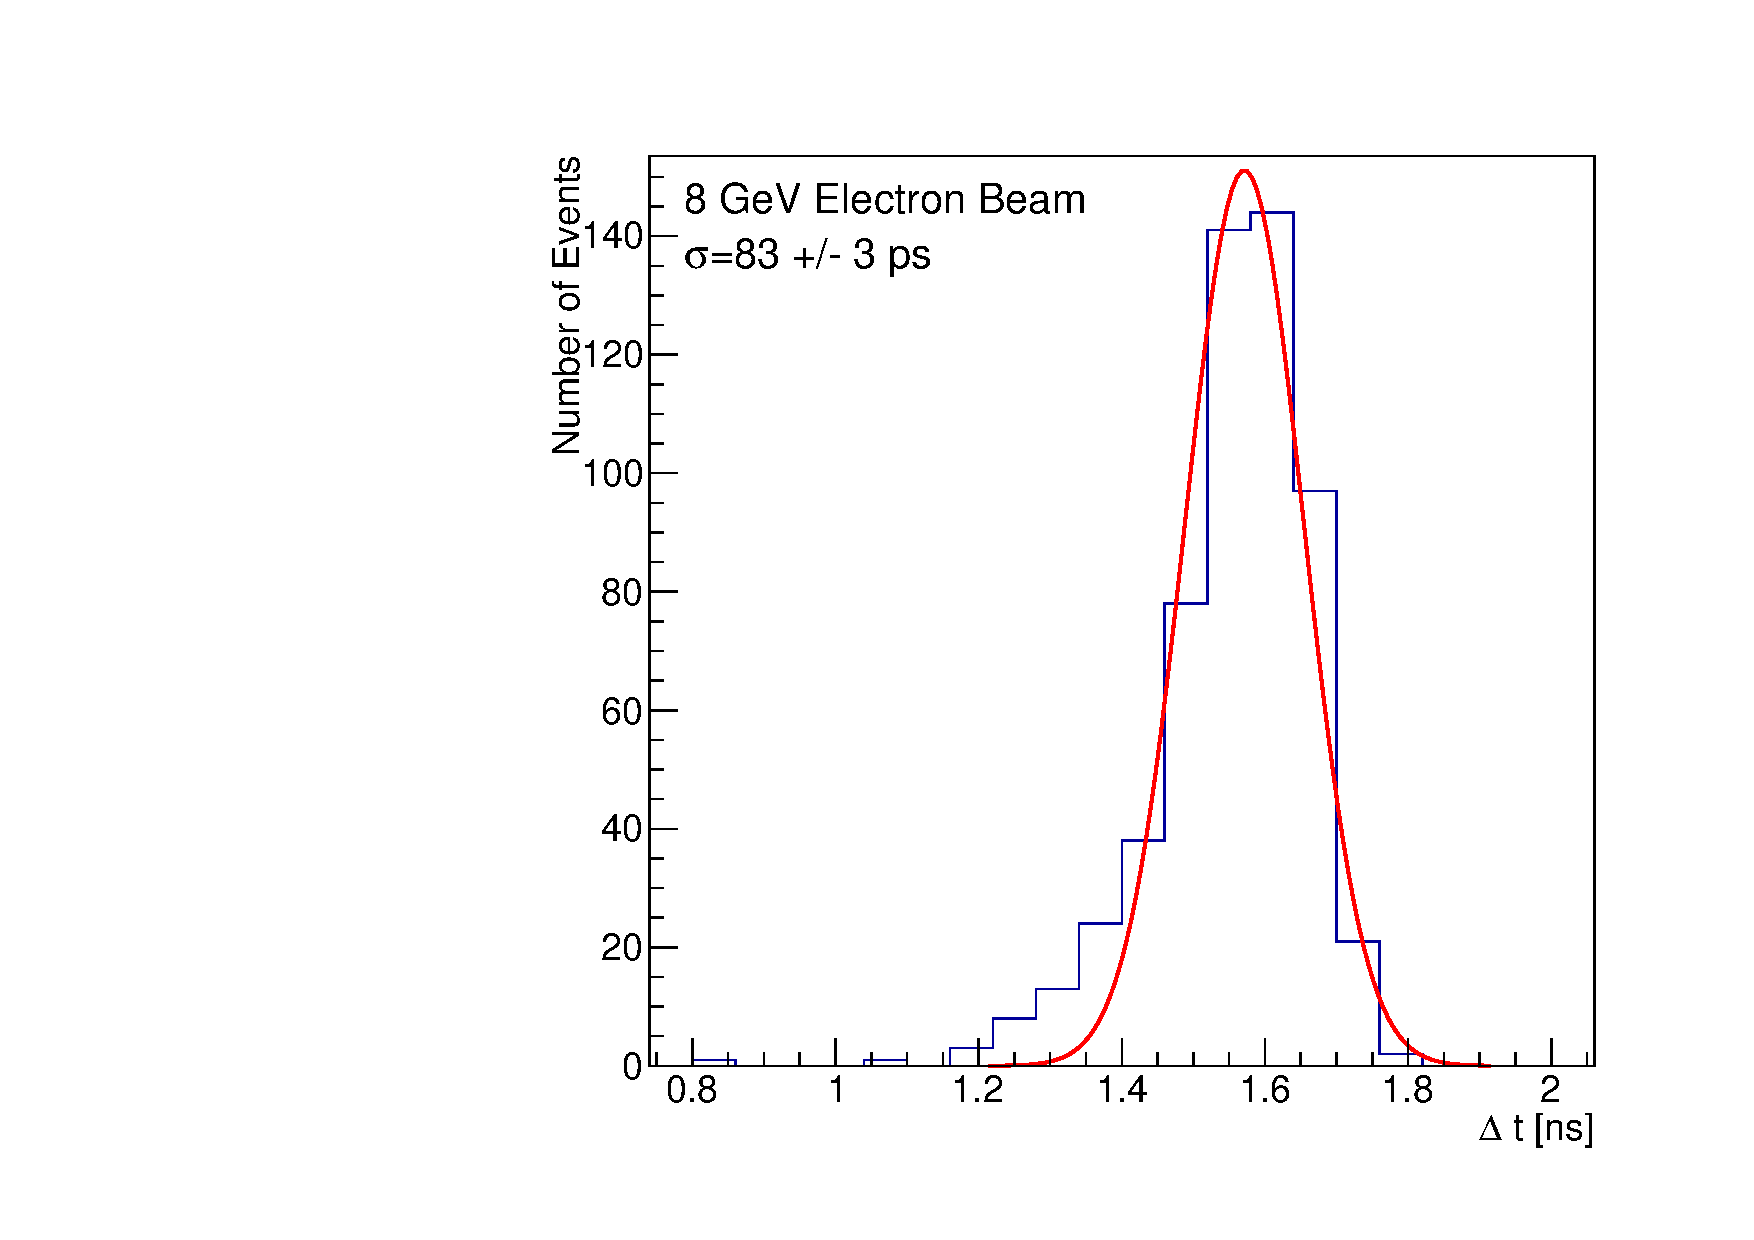
\includegraphics[width=0.45\textwidth]{figs/TOF_ShashlikSideReadout_Electron_8GeV} 
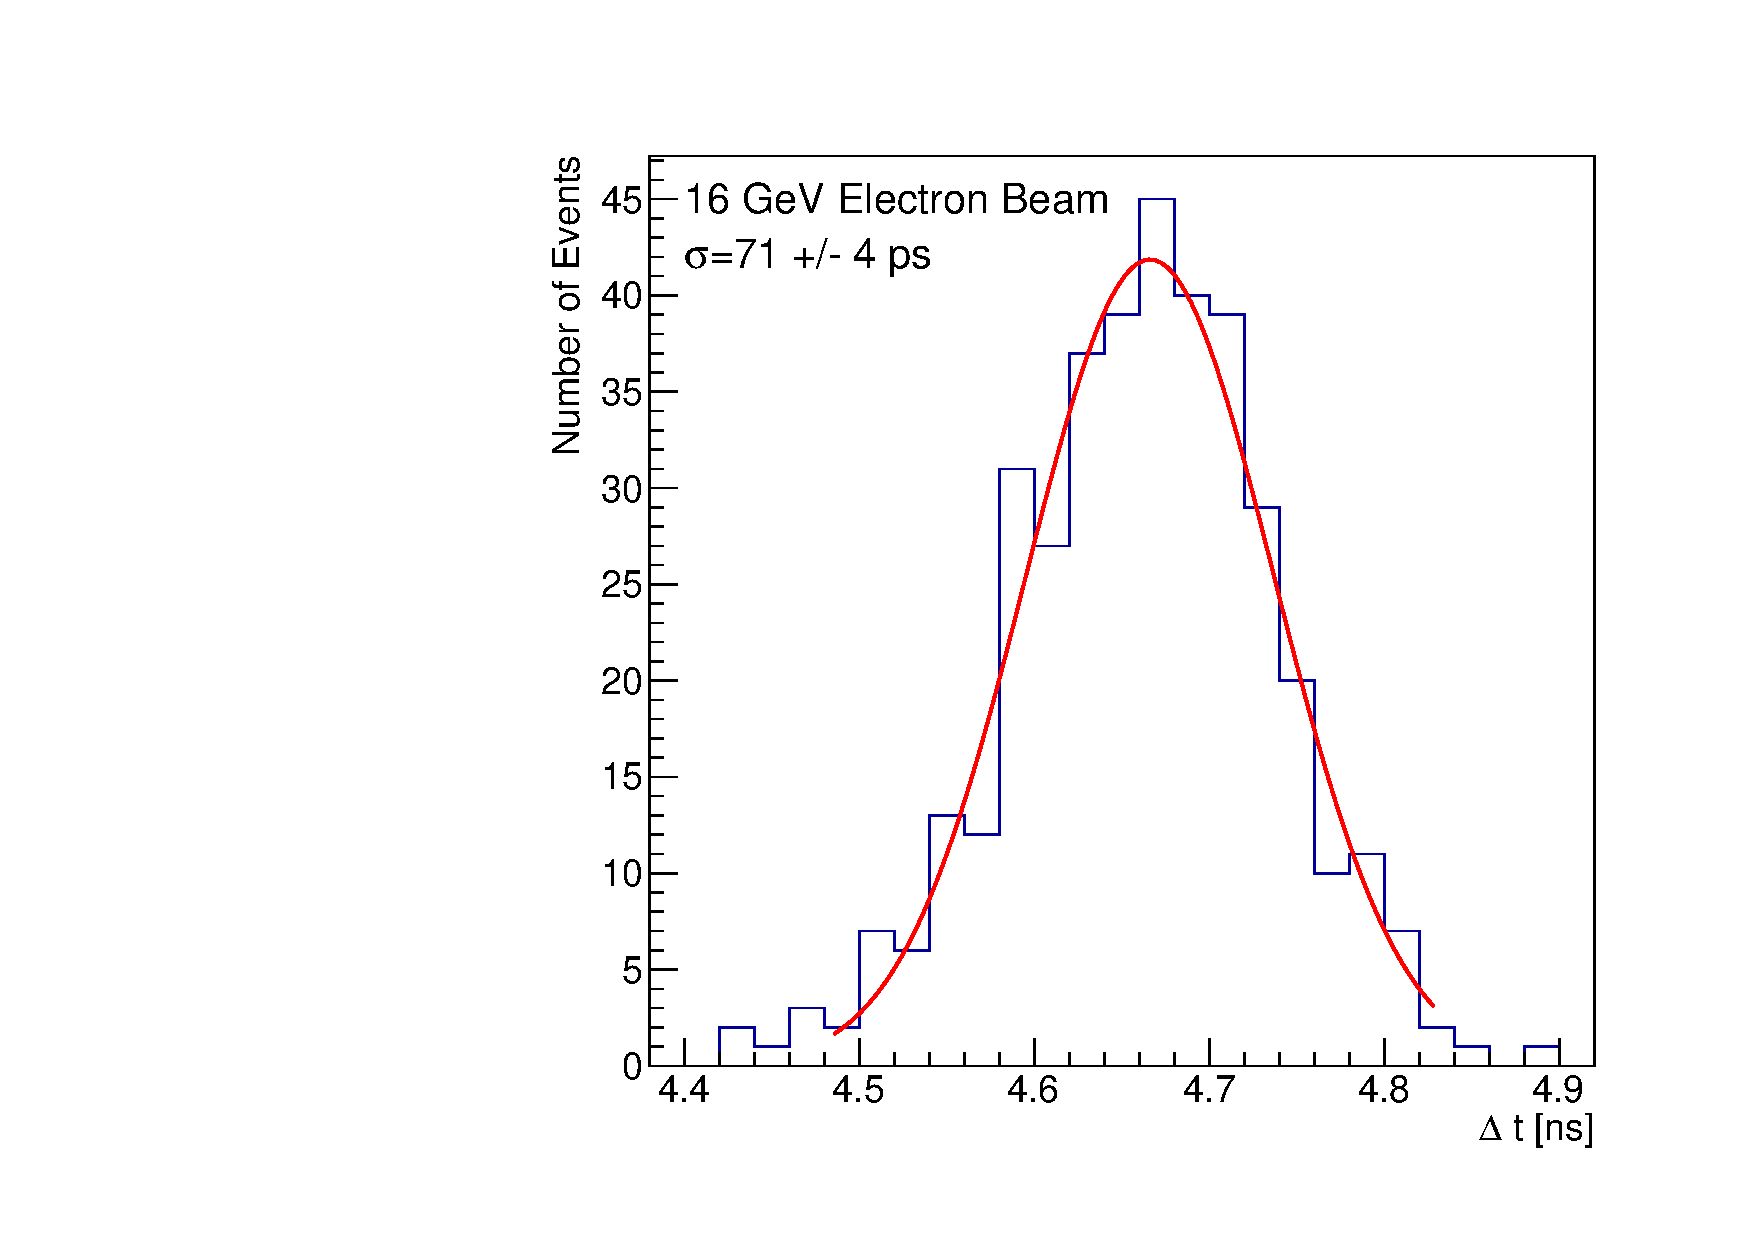
\includegraphics[width=0.45\textwidth]{figs/TOF_ShashlikSideReadout_Electron_16GeV} 
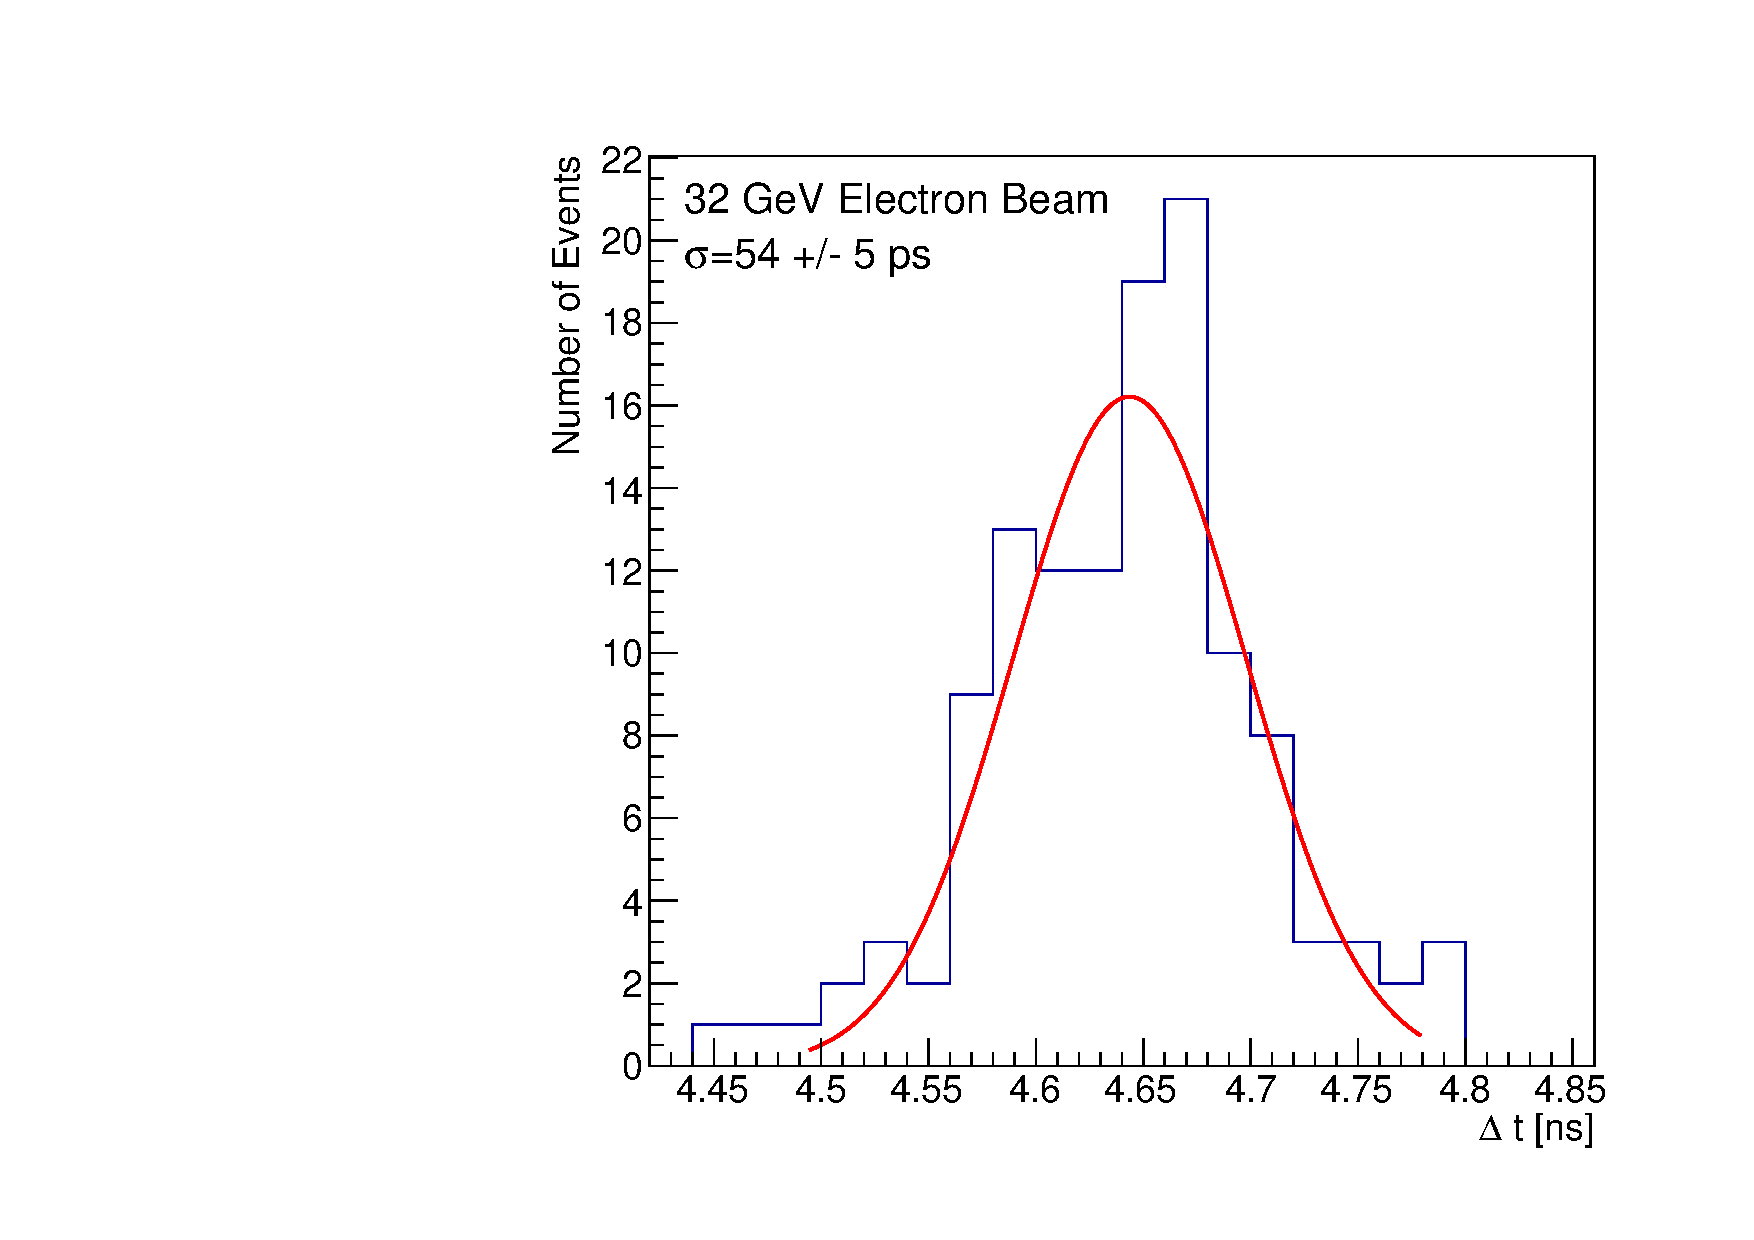
\includegraphics[width=0.45\textwidth]{figs/TOF_ShashlikSideReadout_Electron_32GeV} 
\caption{ Time of flight distributions for the LYSO-tungsten shashlik calorimeter
with signal extracted from the edges of two LYSO layers. } 
\label{fig:ShashlikSideReadoutTOF}
\end{figure}

\begin{figure}[H] \centering
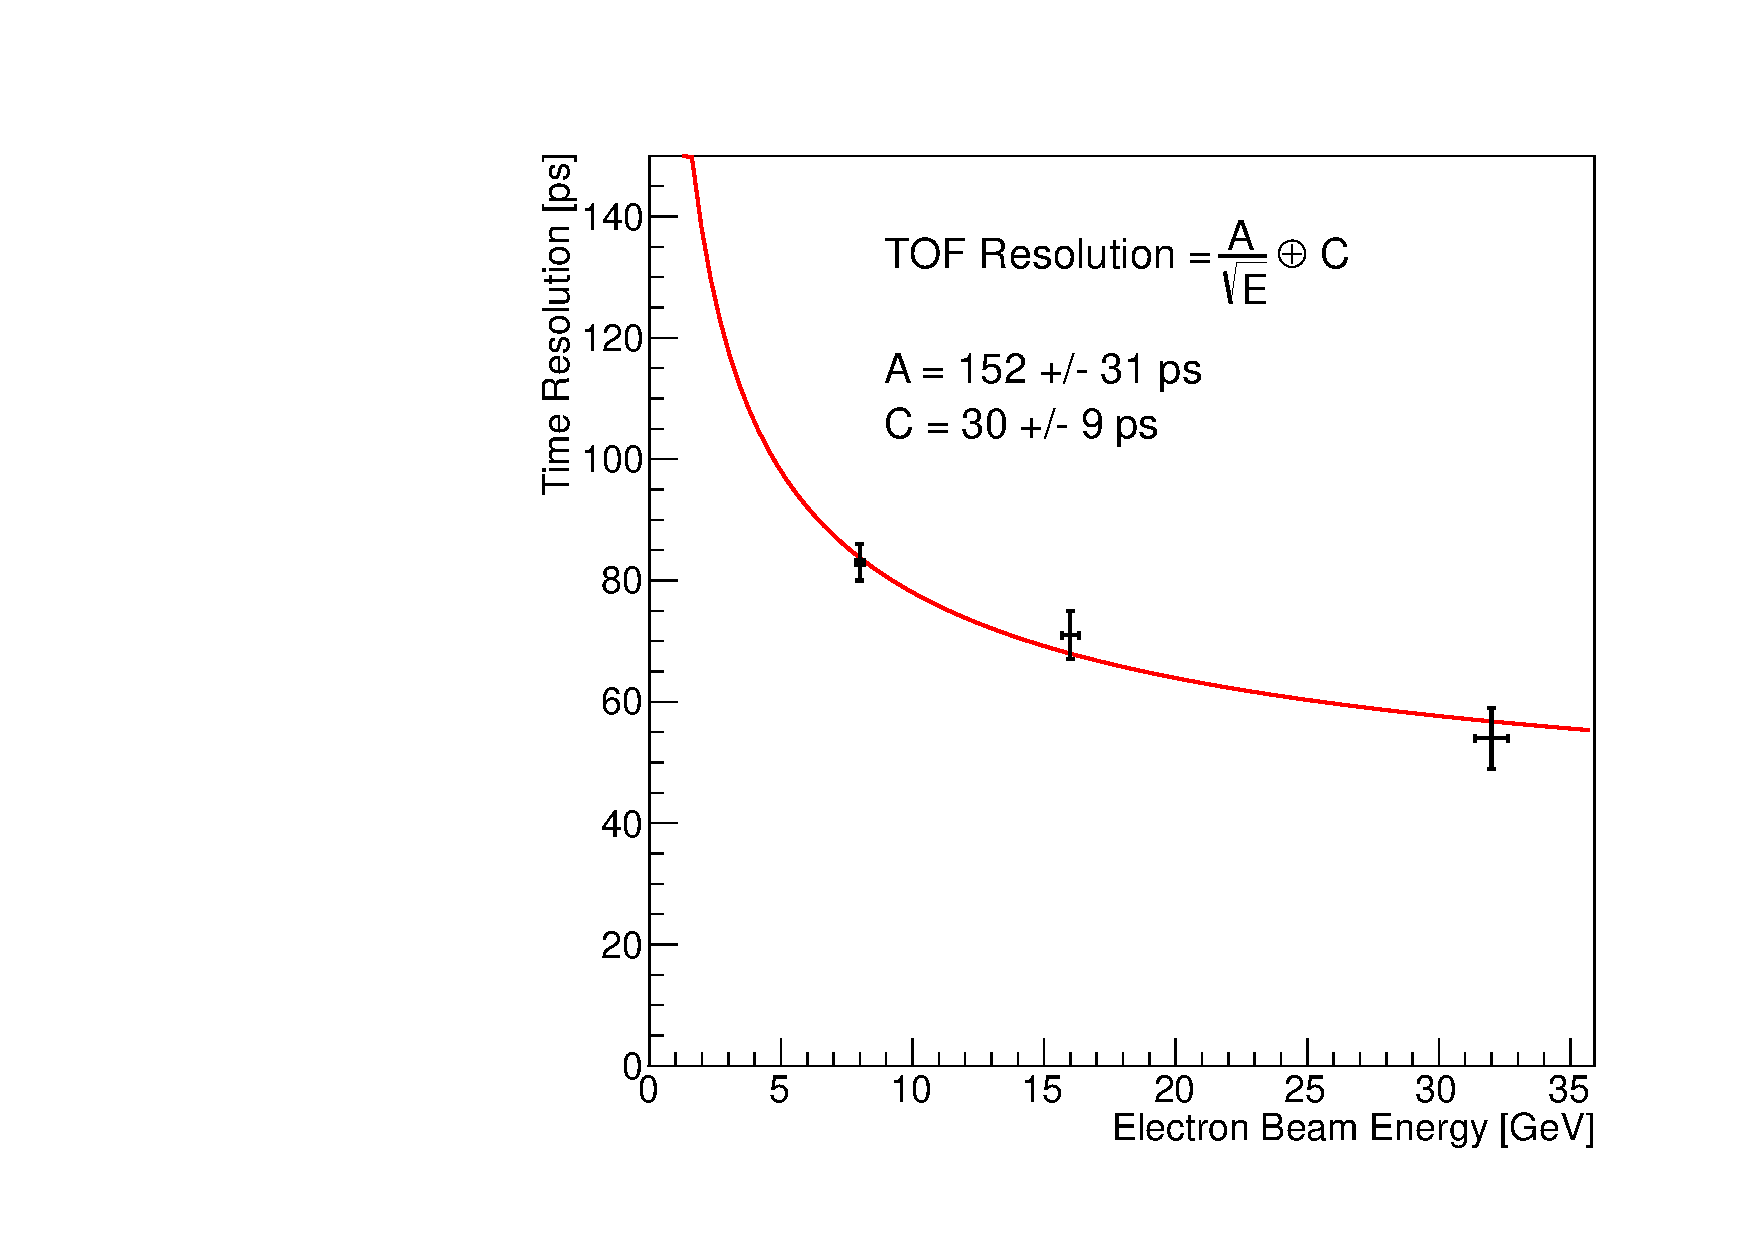
\includegraphics[width=0.45\textwidth]{figs/TimeResolutionVsEnergy_ShashlikSideReadout} 
\caption{ The time resolution measured using the LYSO-tungsten shashlik calorimeter
with light signals extracted by direct optical coupling to the edges of two LYSO layers 
is plotted as a function of the electron beam energy, and fitted to the sum 
of a $1/\sqrt{E}$ term and a constant term. }
\label{fig:ShashlikSideReadoutTOFResolutionVsEnergy}
\end{figure}

In summary, we find that removing the impact of the wavelength shifting
mechanism and minimizing the impact of optical transit does indeed improve the
time resolution, but at a cost in photostatistics. Results obtained in this
experiment suggest that a LYSO-tungsten shashlik calorimeter with edge readout
can likely achieve $30$~ps resolution provided some improvement to the light
collection efficiency is achieved.

\section{Summary}

In this article we have described studies characterizing the timing performance
of LYSO-based calorimeters. Using a (1.7~cm)$^{3}$ LYSO crystal that
samples the electromagnetic showers created by electrons of various energies
ranging from $4$~GeV to $32$~GeV at about $4.5$~$X_{0}$, we inferred that the
contribution to the time resolution from event-by-event fluctuations of the
shower profile, the scintillation process, and the optical transit was less than
$30$~ps. Studies of the effect of optical transit through WLS fibers in a
LYSO-tungsten Shashlik calorimeter demonstrated that the choice of WLS fiber has
a major impact on the timing performance. Besides the absorption and re-emission
processes in the WLS fibers, we found that another important factor influencing
the timing performance is the light extraction efficiency. Using DSB1 fibers, we
obtained a best time resolution of about $100$~ps, and found that the time
resolution remains photostatistics limited. Therefore, future development of
such a detector should be focused on increasing the light collection efficiency.
Finally, using a scheme in which the scintillation light from the LYSO-tungsten
Shashlik calorimeter was extracted via the edges of two LYSO layers, thereby
removing the impact of the wavelength shifting mechanism, we achieved a best
time resolution of $55$~ps. This result gave some indication that such a
calorimeter design would likely be able to achieve a $30$~ps time resolution
provided some improvement to the light collection efficiency is achieved.

Through the comparison of results using these different light extraction
schemes, we found that at a given light yield the effect of optical transit
fluctuations is of considerable importance, but that these effects have a
tendency to decrease in importance as the light yield increases. This effect can
be seen in Figure~\ref{fig:ShashlikFiberAndCubeTOF} where we show the dependence
of the time resolution for the shashlik cell with light extracted through the
DSB1 fibers and for the sampling calorimeter with the $(1.7$~cm$)^{3}$ LYSO cube
as active element as a function of the average pulse height. For the same
average pulse height, a difference of a factor of two is observed in the
measured time resolutions, primarily due to optical transit effects. However, as
the pulse height increases, the time resolution also improves. Extrapolating to
the regime of very large light yield, we have not observed any evidence of an
ultimate limitation in resolution resulting from optical transit fluctuations.

\begin{figure}[H] \centering
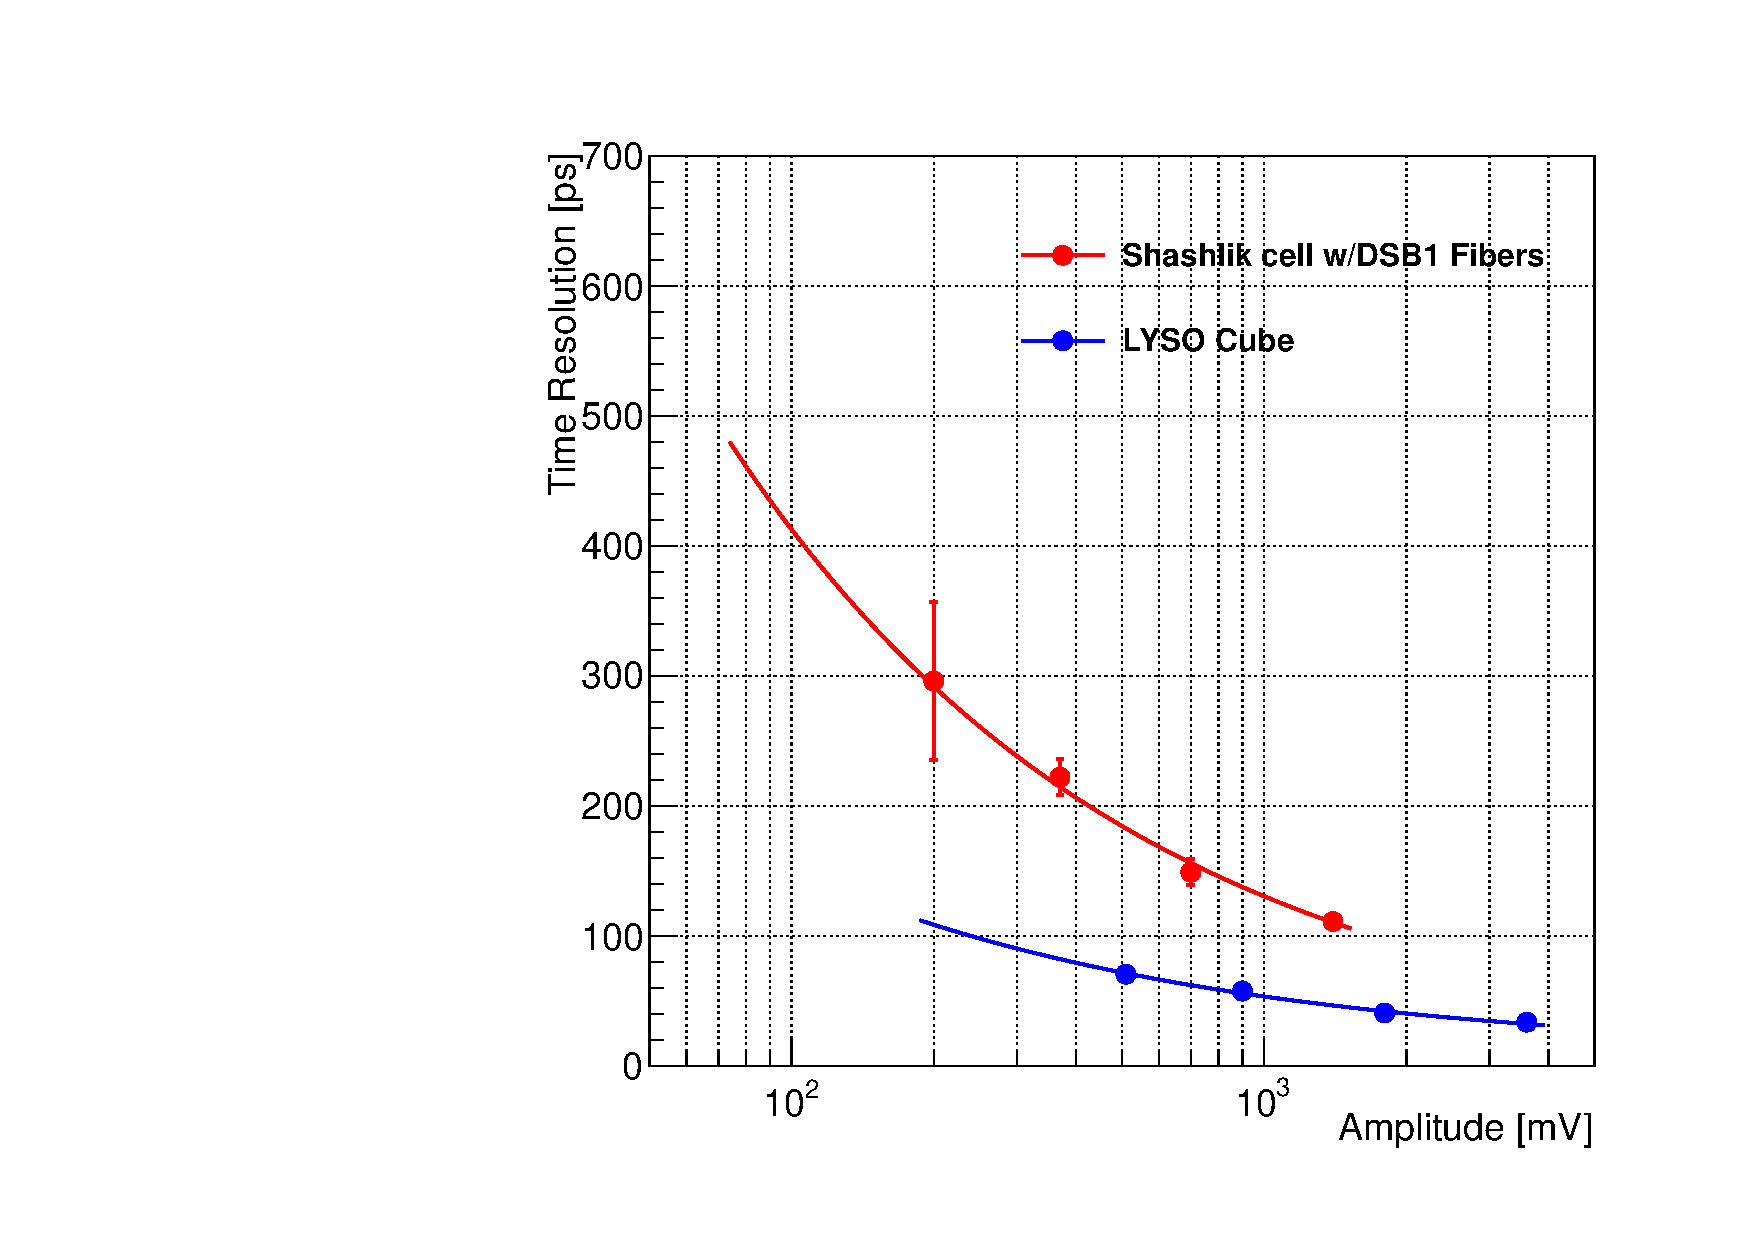
\includegraphics[width=0.55\textwidth]{figs/TimeResolutionVsEnergy_ShashlikDSB1FiberAndCube} 
\caption{Comparison of time resolutions obtained with the $(1.7$~cm$)^{3}$ LYSO cube (blue), 
and the LYSO-tungsten shashlik calorimeter with light extracted using DSB1 fibers (red). 
Attenuators have been used to extend the dynamic range of the
DRS4 waveform digitizer. The x-axis in this figure displays the amplitude of the
signal, corrected for the attenuation factors. }
\label{fig:ShashlikFiberAndCubeTOF}
\end{figure}

In summary, at the light yield achieved, all factors influencing the time
resolution were controlled to within $30$~ps, and the goal of obtaining $30$~ps
resolution time measurements using a LYSO-based calorimeter was achieved. The
next step will be to investigate any ultimate limitation in time resolution in
the limit of very large light yield, and to make improvements to the light
collection efficiency in these kinds of detectors.

\section{Acknowledgements} We would like to thank Erik Ramberg and Sergey Los
for their support of our work, and Aria Soha and the FTBF test beam facility for
the good beam delivery and control. We thank Randy Ruchti for providing us with
the DSB1 fibers used in the measurements, and Eileen Hahn for the high quality
work in polishing the fibers. Thanks to Ewa Skup and Geoff Savage for help with
operation of Cherenkov counters, and to Todd Nobel for organizing and providing
supporting equipment at FTBF.


\bibliography{FastTimingPaperAug2014}{}
\bibliographystyle{ieeetr}
\end{document}    
        






























